\documentclass[12pt]{report}

% ================== PACKAGES ==================
\usepackage[utf8]{inputenc}
\usepackage[T1]{fontenc}
\usepackage[english]{babel} 

% Layout and formatting
\usepackage[a4paper, left=3cm, right=2.5cm, top=3cm, bottom=3cm]{geometry}
\usepackage{setspace}
\onehalfspacing

% Math and algorithm
\usepackage{amsmath}
\usepackage{amssymb}
\usepackage{algorithm}
\usepackage{algpseudocode}
\usepackage{amsthm}

% Figures and tables
\usepackage{graphicx}
\usepackage{float}
\usepackage{placeins}
\usepackage{caption}
\usepackage{subcaption}

% Listings
\usepackage{listings}
\usepackage{xcolor}

% Hyperlink
\usepackage{hyperref}

% Text enhancements
\usepackage{textcomp}
\usepackage{gensymb}
\usepackage{enumitem}
\usepackage{tabto}

% Background (optional, check usage)
\usepackage{background}

% ================== THEOREM STYLES ==================
\newtheorem{definition}{Definition}[section]
\newtheorem{theorem}{Theorem}[chapter]

% ================== LISTING SETUP ==================
\lstset{
    language=Python,
    basicstyle=\ttfamily\scriptsize,
    keywordstyle=\color[rgb]{0.878, 0.467, 0.0},
    commentstyle=\color[rgb]{0.5,0.5,0.5},
    stringstyle=\color[rgb]{0, 0.4, 0},
    identifierstyle=\color[rgb]{0.0, 0.298, 0.380},
    numbers=left,
    numberstyle=\tiny\color{gray},
    stepnumber=1,
    numbersep=5pt,
    showstringspaces=false,
    breaklines=true,
    frame=single,
    rulecolor=\color{black},
    captionpos=b
}
\begin{document}
\backgroundsetup{
  scale=1,
  color=black,
  opacity=0.8,
  angle=0,
  position=current page.center,
  contents={}
}

% ----- Cover Page -----
\begin{titlepage}
	\backgroundsetup{
    scale=1,
    color=black,
    opacity=1,
    angle=0,
    position=current page.center,
    contents={%
    
\includegraphics[width=\paperwidth,height=\paperheight]{background.png}
    }
}
    \centering
    \textbf{\small POSTS AND TELECOMMUNICATIONS INSTITUTE OF TECHNOLOGY}\\ % Translated
    \textbf{\normalsize FACULTY OF INFORMATION TECHNOLOGY I}\\ % Translated
    \centerline{--------------------o0o--------------------}
    \vspace{1cm}
    
\includegraphics[width=8cm]{logo.png}\\
    \vspace{1cm}
{\Large \textbf{PROJECT REPORT 1}}\\[0.5cm] % Translated
{\LARGE \textbf{PYTHON PROGRAMMING LANGUAGE}}\\ % Translated
    \vfill
    \begin{flushleft}
    \hspace{2.5cm}\textbf{Instructor:} \hspace{2.85cm} Kim Ngoc Bach \\ % Translated
    \hspace{2.5cm}\textbf{Student:} \hspace{3.3cm} Dong Duc Nguyen\\ % Translated
    \hspace{2.5cm}\textbf{Student ID:} \hspace{2.7cm} B23DCVT311\\ % Translated
   \hspace{2.5cm}\textbf{Class:} \hspace{3.9cm} D23CQCEO6-B\\ % Translated
    \hspace{2.5cm}\textbf{Course Year:} \hspace{2.4cm} 2023 - 2028 \\ % Translated
    \hspace{2.5cm}\textbf{Training System:} \hspace{1.6cm} Full-time University\\ % Translated
    \end{flushleft}
    \vfill
    {\large Hanoi, 2025} % Translated
\end{titlepage}

\clearpage
% ----- Cover Page -----
\begin{titlepage}
	\backgroundsetup{
    scale=1,
    color=black,
    opacity=1,
    angle=0,
    position=current page.center,
    contents={%
    
\includegraphics[width=\paperwidth,height=\paperheight]{background.png}
    }
}
    \centering
    \textbf{\small POSTS AND TELECOMMUNICATIONS INSTITUTE OF TECHNOLOGY}\\ % Translated
    \textbf{\normalsize FACULTY OF INFORMATION TECHNOLOGY I}\\ % Translated
    \centerline{--------------------o0o--------------------}
    \vspace{1cm}
    
\includegraphics[width=8cm]{logo.png}\\
    \vspace{1cm}
{\Large \textbf{PROJECT REPORT 1}}\\[0.5cm] % Translated
{\LARGE \textbf{PYTHON PROGRAMMING LANGUAGE}}\\ % Translated
    \vfill
    \begin{flushleft}
    \hspace{2.5cm}\textbf{Instructor:} \hspace{2.85cm} Kim Ngoc Bach \\ % Translated
    \hspace{2.5cm}\textbf{Student:} \hspace{3.3cm} Dong Duc Nguyen\\ % Translated
    \hspace{2.5cm}\textbf{Student ID:} \hspace{2.7cm} B23DCVT311\\ % Translated
   \hspace{2.5cm}\textbf{Class:} \hspace{3.9cm} D23CQCEO6-B\\ % Translated
    \hspace{2.5cm}\textbf{Course Year:} \hspace{2.4cm} 2023 - 2028 \\ % Translated
    \hspace{2.5cm}\textbf{Training System:} \hspace{1.6cm} Full-time University\\ % Translated
    \end{flushleft}
    \vfill
    {\large Hanoi, 2025} % Translated
\end{titlepage}
\clearpage
\newgeometry{top=2.5cm,bottom=2cm,left=3cm,right=2cm}
\thispagestyle{empty}
\begin{center}
	{\textbf{\Large{INSTRUCTOR'S COMMENTS}}} % Translated
\end{center}

\dotfill \vspace{0.25cm} \par
\dotfill \vspace{0.25cm} \par
\dotfill \vspace{0.25cm} \par
\dotfill \vspace{0.25cm} \par
\dotfill \vspace{0.25cm} \par
\dotfill \vspace{0.25cm} \par
\dotfill \vspace{0.25cm} \par
\dotfill \vspace{0.25cm} \par
\dotfill \vspace{0.25cm} \par
\dotfill \vspace{0.25cm} \par
\dotfill \vspace{0.25cm} \par
\dotfill \vspace{0.25cm} \par
\dotfill \vspace{0.25cm} \par
\dotfill \vspace{0.25cm} \par
\dotfill \vspace{0.25cm} \par
\dotfill \vspace{0.25cm} \par
\dotfill \vspace{0.25cm} \par
\dotfill \vspace{0.25cm} \par
\dotfill
\vspace{1cm}

{\textbf{\large{Score: }}} \hspace{1.0cm}\textbf{( In words:} \hspace{2.5cm}\textbf{)} % Translated

\begin{flushright}
	Hanoi, date \hspace{0.75cm} month \hspace{0.75cm} year 20...\hspace{0.75cm} % Translated

	{\textbf{\large{Instructor}}} \hspace{2cm} \textcolor{white}{.} % Translated
\end{flushright}
\clearpage
\tableofcontents
\newpage
\listoffigures
\newpage
\chapter*{INTRODUCTION} % Translated
{
\noindent
In the digital era, the ability to collect, process, and analyze data has become an essential skill in many fields, including sports. The Python programming language, with its rich and powerful library ecosystem such as \texttt{Pandas}, \texttt{Scikit-learn}, \texttt{Selenium}, and \texttt{BeautifulSoup}, provides effective tools to solve complex data analysis problems. This Major Project Report for the \textit{Python Programming Language} course focuses on applying Python to perform a series of tasks related to football data analysis, specifically from the English Premier League.
\vspace{1em}
\noindent
\textbf{The main objectives of the report include:} % Translated
\begin{itemize}
  \item Collecting detailed statistical data of players from reliable online sources (\texttt{fbref.com}, \texttt{footballtransfers.com}) using web scraping techniques.
\item Performing descriptive statistical analyses to explore the data, identify outstanding players, and characteristics of the teams.
\item Applying unsupervised machine learning algorithms (K-means) combined with dimensionality reduction techniques (PCA) to classify players into groups based on their playing characteristics.
\item Building a supervised machine learning model (\texttt{Random Forest Regressor}) to estimate player transfer values based on statistical indicators and personal information.
\end{itemize}

\vspace{0.5em}
\noindent
The report is structured into four main parts (Problem I, II, III, IV), each addressing a specific requirement mentioned above. By performing these tasks, the report not only illustrates the applicability of Python in sports data analysis but also provides deep insights into player performance and transfer market dynamics.
}
\chapter{PROBLEM I} % Translated
{
\section{Requirement} % Translated
\begin{itemize}
	\item Collect statistical data [*] for all players who have played more than 90 minutes in the 2024-2025 English Premier League season.
\item Data source: https://fbref.com/en/
	\item Save the result to a file named 'results.csv', where the result table has the following structure:
	\begin{itemize}
		\item Each column corresponds to a statistic.
\item Players are sorted alphabetically by their first name.
		\item Any statistic that is unavailable or inapplicable should be marked as "N/a".
\end{itemize}
\end{itemize}
\begin{itemize}
    \item[*] The required statistics are:
    \begin{itemize}
        \item Nation
        \item Team
        \item Position
        \item Age
        \item Playing Time: matches played, starts, minutes
        \item Performance: goals, assists, yellow cards, red cards
        \item Expected: expected goals (xG), expected Assist Goals (xAG)
 \item Progression: PrgC, PrgP, PrgR
        \item Per 90 minutes: Gls, Ast, xG, xGA
        \item Goalkeeping:
        \begin{itemize}
            \item Performance: goals against per 90mins (GA90), Save\%, CS\%
            \item Penalty Kicks: penalty kicks Save\%
        \end{itemize}
        \item Shooting:
        \begin{itemize}
           \item Standard: shots on target percentage (SoT\%), Shot on Target per 90min (SoT/90), goals/shot (G/Sh), average shot distance (Dist)
        \end{itemize}
        \item Passing:
        \begin{itemize}
            \item Total: passes completed (Cmp), pass completion (Cmp\%), progressive passing distance (TotDist)
            \item Short: pass completion (Cmp\%)
     \item Medium: pass completion (Cmp\%)
            \item Long: pass completion (Cmp\%)
            \item Expected: key passes (KP), pass into final third ($1/3$), pass into penalty area (PPA), CrsPA, PrgP
        \end{itemize}
        \item Goal and Shot Creation:
        \begin{itemize}
            \item SCA: SCA, SCA90
        \item GCA: GCA, GCA90
        \end{itemize}
        \item Defensive Actions:
        \begin{itemize}
            \item Tackles: Tkl, TklW
            \item Challenges: Att, Lost
            \item Blocks: Blocks, Sh, Pass, Int
        \end{itemize}
\item Possession:
        \begin{itemize}
            \item Touches: Touches, Def Pen, Def 3rd, Mid 3rd, Att 3rd, Att Pen
            \item Take-Ons: Att, Succ\%, Tkld\%
            \item Carries: Carries, ProDist, ProgC, $1/3$, CPA, Mis, Dis
            \item Receiving: Rec, PrgR
        \end{itemize}
\item Miscellaneous Stats:
        \begin{itemize}
            \item Performance: Fls, Fld, Off, Crs, Recov
            \item Aerial Duels: Won, Lost, Won\%
        \end{itemize}
        \item Reference: \url{https://fbref.com/en/squads/822bd0ba/Liverpool-Stats}
    \end{itemize}
\end{itemize}

\section{Implementation Steps} % Translated
	\begin{enumerate}
		\item Initialize data fields:
		\begin{itemize}
			\item Identify the information to be collected (the fields).
\item Create a player dictionary (or class) with the default value 'N/a'.
\item Create a dictionary to store all players by name + team.
\end{itemize}
		\item Retrieve data:
		\begin{itemize}
			\item Retrieve basic data from the summary page (https://fbref.com/en/comps/9/stats/Premier-League-Stats) to initialize the player count, filtering out players who did not play more than 90 minutes.
Add to the dictionary to prepare for updates.
			\item Update data according to requirements (only update players present in the dictionary).
\item Update according to each required section to ensure completeness.
\end{itemize}
		\item Export data:
		\begin{itemize}
			\item Export fields according to the requirements (convert to a list containing content as required).
\item Fix the data into a DataFrame.
			\item Export data to the 'results.csv' file.
		\end{itemize}
	\end{enumerate}

\section{Actual Code and Detailed Description} % Translated
\subsection{Main Function} % Translated
\begin{lstlisting}
def Problem_1():

	print("Starting to retrieve basic data...")
	player_set_dict = create_Set_Players()
	print(f"Retrieved basic data for {len(player_set_dict)} players.")

	print("Updating goalkeeping data...")
	update_Set_Goalkeeping(player_set_dict)
	print("Updating shooting data...")
	update_Set_Shooting(player_set_dict)
	print("Updating passing data...")
	update_Set_Passing(player_set_dict)
	print("Updating goal and shot creation data...")
	update_Set_Goal_And_Shot_Creation_Data(player_set_dict)
	print("Updating defensive actions data...")
	update_Set_Defensive_Actions_Data(player_set_dict)
	print("Updating possession data...")
	update_Set_Possession(player_set_dict)
	print("Updating miscellaneous data...")
	update_Set_Miscellaneous_Data(player_set_dict)
	print("Data update completed.")

	export(player_set_dict)
	print("Program completed.")
\end{lstlisting}
\textbf{Operations are similar to those in the implementation steps section:} % Translated
\textbf{$create\_Set\_Players()$} This is the initialization function that also retrieves basic data from the summary page to create a dictionary of all players who have played more than 90 minutes. Retrieves data from https://fbref.com/en/comps/9/stats/Premier-League-Stats.
\textbf{Operations:} % Translated
\begin{flushleft}
\texttt{update\_Set\_Goalkeeping(player\_set\_dict)}\\
\texttt{update\_Set\_Shooting(player\_set\_dict)}\\
\texttt{update\_Set\_Passing(player\_set\_dict)}\\
\texttt{update\_Set\_Goal\_And\_Shot\_Creation\_Data(player\_set\_dict)}\\
\texttt{update\_Set\_Defensive\_Actions\_Data(player\_set\_dict)}\\
\texttt{update\_Set\_Possession(player\_set\_dict)}\\
\texttt{update\_Set\_Miscellaneous\_Data(player\_set\_dict)}\\
\end{flushleft}
These are the operations during the process of updating the required data: % Translated

\begin{itemize}
	\item update\_Set\_Goalkeeping(player\_set\_dict): operation to update Goalkeeping data, retrieving from: https://fbref.com/en/comps/9/keepers/Premier-League-Stats
	\item update\_Set\_Shooting(player\_set\_dict): operation to update Shooting data, retrieving from: https://fbref.com/en/comps/9/shooting/Premier-League-Stats
	\item update\_Set\_Passing(player\_set\_dict): operation to update Passing data, retrieving from: https://fbref.com/en/comps/9/passing/Premier-League-Stats
	\item update\_Set\_Goal\_And\_Shot\_Creation\_Data(player\_set\_dict): operation to update Goal And Shot Creation data, retrieving from: https://fbref.com/en/comps/9/gca/Premier-League-Stats
	\item update\_Set\_Defensive\_Actions\_Data(player\_set\_dict): operation to update Defensive Actions data, retrieving from: https://fbref.com/en/comps/9/defense/Premier-League-Stats
	\item update\_Set\_Possession(player\_set\_dict): operation to update Possession data, retrieving from: https://fbref.com/en/comps/9/possession/Premier-League-Stats
	\item update\_Set\_Miscellaneous\_Data(player\_set\_dict): operation to update Miscellaneous data, retrieving from: https://fbref.com/en/comps/9/misc/Premier-League-Stats
\end{itemize}
\textbf{export(player\_set\_dict):} operation to fix data into a DataFrame and export to the 'results.csv' file as required.
\subsection{Detailed Operations} % Translated
\textbf*{Initialize dictionaries containing player information:} % Translated
\lstset{
    language=Python,
    basicstyle=\ttfamily\scriptsize,
    keywordstyle=\color[rgb]{0.878, 0.467, 0.0}, % dark blue for keyword
    commentstyle=\color[rgb]{0.5,0.5,0.5}, % gray for comment
    stringstyle=\color[rgb]{0, 0.4, 0},
 identifierstyle=\color[rgb]{0.0, 0.298, 0.380}, % normal for variable
    numbers=left,
    numberstyle=\tiny\color[rgb]{0.5,0.5,0.5},
    numbersep=5pt,
    showstringspaces=false,
    breaklines=true,
    tabsize=2
}
\begin{lstlisting}
PLAYER_KEYS = ['name', 'nationality', 'position', 'team', 'age', 'games', 'games_starts', 'minutes', 'goals', 'assist', 'cards_yellow', 'cards_red', 'xg', 'xg_assist', 'progressive_carries', 'progressive_passes', 'progressive_passes_received', 'goals_per90', 'assists_per90', 'xg_per90', 'xg_assist_per90', 'gk_goals_against_per90', 'gk_save_pct', 'gk_clean_sheets_pct', 'gk_pens_save_pct', 'shots_on_target_pct', 'shots_on_target_per90', 'goals_per_shot', 'average_shot_distance', 'passes_completed', 'passes_pct', 'passes_total_distance', 'passes_pct_short', 'passes_pct_medium', 'passes_pct_long', 'assisted_shots', 'passes_into_final_third', 'passes_into_penalty_area', 'crosses_into_penalty_area', 'sca', 'sca_per90', 'gca', 'gca_per90', 'tackles', 'tackles_won', 'challenges', 'challenges_lost', 'blocks', 'blocked_shots', 'blocked_passes', 'interceptions', 'touches', 'touches_def_pen_area', 'touches_def_3rd', 'touches_mid_3rd', 'touches_att_3rd', 'touches_att_pen_area', 'take_ons', 'take_ons_won_pct', 'take_ons_tackled_pct', 'carries', 'carries_progressive_distance', 'carries_into_final_third',
'carries_into_penalty_area', 'miscontrols', 'dispossessed', 'passes_received', 'fouls', 'fouled', 'offsides', 'crosses', 'ball_recoveries', 'aerials_won', 'aerials_lost', 'aerials_won_pct']

def create_default_player_dict(): return {key: 'N/a' for key in PLAYER_KEYS}

\end{lstlisting}
This operation aims to create a player dictionary with the attributes listed in PLAYER\_KEYS, which have been previously declared. We set the initial value for all data to 'N/a' so that any values not found (unavailable or inapplicable) will default to this value.

\textbf*{create\_Set\_Players() - Create player dictionary:} % Translated
\begin{lstlisting}
def create_Set_Players():
    driver = webdriver.Chrome()
    url = 'https://fbref.com/en/comps/9/stats/Premier-League-Stats'
    driver.get(url)
    page_source = driver.page_source
    soup = BeautifulSoup(page_source, 'html.parser')
    x = soup.find('table', attrs={'id': 'stats_standard'})
cnt = 0
    player_set = {}
    for i in range(589):
        cnt += 1
        if cnt == 26:
            cnt = 0
            continue
        table = x.find('tr', attrs={'data-row': f'{str(i)}'})
        if not table:
            continue
  player_data = create_default_player_dict()
        player_data['name'] = table.find('td', attrs={'data-stat': 'player'}).text.strip()
        player_data['nationality'] = table.find('td', attrs={'data-stat': 'nationality'}).text.strip()
        player_data['position'] = table.find('td', attrs={'data-stat': 'position'}).text.strip()
        player_data['team'] = table.find('td', attrs={'data-stat': 'team'}).text.strip()
        player_data['age'] = table.find('td', attrs={'data-stat': 'age'}).text.strip()
        player_data['games'] = table.find('td', attrs={'data-stat': 'games'}).text.strip()
        player_data['games_starts'] = table.find('td', attrs={'data-stat': 'games_starts'}).text.strip()
        minutes_str = table.find('td', attrs={'data-stat':
'minutes'}).text.strip()
        player_data['minutes'] = minutes_str
        minutes_str_cleaned = minutes_str.replace(',', '')
        if int(minutes_str_cleaned) <= 90:
            continue
        player_data['goals'] = table.find('td', attrs={'data-stat': 'goals'}).text.strip()
        player_data['assist'] = table.find('td', attrs={'data-stat': 'assists'}).text.strip()
        player_data['cards_yellow'] = table.find('td', attrs={'data-stat': 'cards_yellow'}).text.strip()
        player_data['cards_red'] = table.find('td', attrs={'data-stat': 'cards_red'}).text.strip()
player_data['xg'] = table.find('td', attrs={'data-stat': 'xg'}).text.strip()
        player_data['xg_assist'] = table.find('td', attrs={'data-stat': 'xg_assist'}).text.strip()
        player_data['progressive_carries'] = table.find('td', attrs={'data-stat': 'progressive_carries'}).text.strip()
        player_data['progressive_passes'] = table.find('td', attrs={'data-stat': 'progressive_passes'}).text.strip()
        player_data['progressive_passes_received'] = table.find('td', attrs={'data-stat': 'progressive_passes_received'}).text.strip()
        player_data['goals_per90'] = table.find('td', attrs={'data-stat': 'goals_per90'}).text.strip()
        player_data['assists_per90'] = table.find('td', attrs={'data-stat': 'assists_per90'}).text.strip()
        player_data['xg_per90'] = table.find('td', attrs={'data-stat': 'xg_per90'}).text.strip()
        player_data['xg_assist_per90'] = table.find('td', attrs={'data-stat':
'xg_assist_per90'}).text.strip()
        player_key = str(player_data['name']) + str(player_data['team'])
        player_set[player_key] = player_data
    driver.quit()
    return player_set
\end{lstlisting}
To avoid being blocked and ensure completeness, accuracy, and prevent failure during data retrieval from the website, use a webdriver from the selenium library, assign it to the variable `driver`, and proceed with data retrieval [lines 2 - 5]. Once the website data is obtained, normalize it using BeautifulSoup [line 6]. End the process of retrieving data from the website. Start the search process. First, to reduce search time, retrieve only the necessary data (the information table into variable `x`) [line 7]. Create a `cnt` variable to skip header rows [lines 8, 11 - 14]. Create a player dataset `player\_set` to store valid players [line 9]. Loop to retrieve all player information. In each loop, create a new dictionary containing the new player's information [line 18]. Find the name, nationality, team, age, matches played, starts, playing time, and assign them to the keys in the dictionary [lines 19 - 27]. Normalize the playing time, then compare; if it's over 90 minutes, continue retrieving the remaining data, otherwise move to the next player. Continue retrieving all data until the end of the table. Assign the newly created dictionary to the dictionary containing all valid players created in line 9, using the player's name + team name as the key. After the loop finishes, quit the driver and return the dictionary containing all valid players created in line 9.

\textbf*{Update functions:} % Translated

\begin{lstlisting}
def update_Set_Goalkeeping(player_set):
    driver = webdriver.Chrome()
    url = 'https://fbref.com/en/comps/9/keepers/Premier-League-Stats'
    driver.get(url)
    page_source = driver.page_source
    soup = BeautifulSoup(page_source, 'html.parser')
    x = soup.find('table', attrs={'id': 'stats_keeper'})
    for i in range (43):
        if i == 25: continue
table = x.find('tr', attrs={'data-row':f'{str(i)}'})
        if not table: continue
        name = table.find('td', attrs={'data-stat':'player'}).text.strip()
        team = table.find('td', attrs={'data-stat':'team'}).text.strip()
        player_key = str(name) + str(team)

        if player_key in player_set:
            player_set[player_key]['gk_goals_against_per90'] = table.find('td', attrs={'data-stat':'gk_goals_against_per90'}).text.strip()
            player_set[player_key]['gk_save_pct'] = table.find('td', attrs={'data-stat':'gk_save_pct'}).text.strip()
 player_set[player_key]['gk_clean_sheets_pct'] = table.find('td', attrs={'data-stat':'gk_clean_sheets_pct'}).text.strip()
            player_set[player_key]['gk_pens_save_pct'] = table.find('td', attrs={'data-stat':'gk_pens_save_pct'}).text.strip()
    driver.quit()

def update_Set_Shooting(player_set):
    driver = webdriver.Chrome()
    url = 'https://fbref.com/en/comps/9/shooting/Premier-League-Stats'
    driver.get(url)
    page_source = driver.page_source
    soup = BeautifulSoup(page_source, 'html.parser')
    x = soup.find('table', attrs={'id': 'stats_shooting'})
    cnt = 0
    for i in range(589):
        cnt+=1
        if cnt==26:
   cnt=0
            continue
        table = x.find('tr', attrs={'data-row':f'{str(i)}'})
        if not table: continue

        name = table.find('td', attrs={'data-stat':'player'}).text.strip()
        team = table.find('td', attrs={'data-stat':'team'}).text.strip()
        player_key = str(name) + str(team)

        if player_key in player_set:
            player_set[player_key]['shots_on_target_pct'] = table.find('td', attrs={'data-stat':'shots_on_target_pct'}).text.strip()
         player_set[player_key]['shots_on_target_per90'] = table.find('td', attrs={'data-stat':'shots_on_target_per90'}).text.strip()
            player_set[player_key]['goals_per_shot'] = table.find('td', attrs={'data-stat':'goals_per_shot'}).text.strip()
            player_set[player_key]['average_shot_distance'] = table.find('td', attrs={'data-stat':'average_shot_distance'}).text.strip()
    driver.quit()

def update_Set_Passing(player_set):
    driver = webdriver.Chrome()
    url = 'https://fbref.com/en/comps/9/passing/Premier-League-Stats'
    driver.get(url)
    page_source = driver.page_source
    soup = BeautifulSoup(page_source, 'html.parser')
    x = soup.find('table', attrs={'id': 'stats_passing'})
    cnt = 0
    for i in range(589):
     cnt+=1
        if cnt==26:
            cnt=0
            continue
        table = x.find('tr', attrs={'data-row':f'{str(i)}'})
        if not table: continue

        name = table.find('td', attrs={'data-stat':'player'}).text.strip()
        team = table.find('td', attrs={'data-stat':'team'}).text.strip()
        player_key = str(name) + str(team)

  if player_key in player_set:
            player_set[player_key]['passes_completed'] = table.find('td', attrs={'data-stat':'passes_completed'}).text.strip()
            player_set[player_key]['passes_pct'] = table.find('td', attrs={'data-stat':'passes_pct'}).text.strip()
            player_set[player_key]['passes_total_distance'] = table.find('td', attrs={'data-stat':'passes_total_distance'}).text.strip()
            player_set[player_key]['passes_pct_short'] = table.find('td', attrs={'data-stat':'passes_pct_short'}).text.strip()
            player_set[player_key]['passes_pct_medium'] = table.find('td', attrs={'data-stat':'passes_pct_medium'}).text.strip()
            player_set[player_key]['passes_pct_long'] = table.find('td', attrs={'data-stat':'passes_pct_long'}).text.strip()
       player_set[player_key]['assisted_shots'] = table.find('td', attrs={'data-stat':'assisted_shots'}).text.strip()
            player_set[player_key]['passes_into_final_third'] = table.find('td', attrs={'data-stat':'passes_into_final_third'}).text.strip()
            player_set[player_key]['passes_into_penalty_area'] = table.find('td', attrs={'data-stat':'passes_into_penalty_area'}).text.strip()
            player_set[player_key]['crosses_into_penalty_area'] = table.find('td', attrs={'data-stat':'crosses_into_penalty_area'}).text.strip()
            player_set[player_key]['progressive_passes'] = table.find('td', attrs={'data-stat':'progressive_passes'}).text.strip()
    driver.quit()


def update_Set_Goal_And_Shot_Creation_Data(player_set):
    driver = webdriver.Chrome()
    url = 'https://fbref.com/en/comps/9/gca/Premier-League-Stats'
    driver.get(url)
    page_source = driver.page_source
 soup = BeautifulSoup(page_source, 'html.parser')
    x = soup.find('table', attrs={'id': 'stats_gca'})
    cnt = 0
    for i in range(589):
        cnt+=1
        if cnt==26:
            cnt=0
            continue
        table = x.find('tr', attrs={'data-row':f'{str(i)}'})
        if not table: continue

        name = table.find('td', attrs={'data-stat':'player'}).text.strip()
       team = table.find('td', attrs={'data-stat':'team'}).text.strip()
        player_key = str(name) + str(team)

        if player_key in player_set:
            player_set[player_key]['sca'] = table.find('td', attrs={'data-stat':'sca'}).text.strip()
            player_set[player_key]['sca_per90'] = table.find('td', attrs={'data-stat':'sca_per90'}).text.strip()
            player_set[player_key]['gca'] = table.find('td', attrs={'data-stat':'gca'}).text.strip()
            player_set[player_key]['gca_per90'] = table.find('td', attrs={'data-stat':'gca_per90'}).text.strip()
    driver.quit()

def update_Set_Defensive_Actions_Data(player_set):
  driver = webdriver.Chrome()
    url = 'https://fbref.com/en/comps/9/defense/Premier-League-Stats'
    driver.get(url)
    page_source = driver.page_source
    soup = BeautifulSoup(page_source, 'html.parser')
    x = soup.find('table', attrs={'id': 'stats_defense'})
    cnt = 0
    for i in range(589):
        cnt+=1
        if cnt==26:
            cnt=0
            continue
        table = x.find('tr',
attrs={'data-row':f'{str(i)}'})
        if not table: continue

        name = table.find('td', attrs={'data-stat':'player'}).text.strip()
        team = table.find('td', attrs={'data-stat':'team'}).text.strip()
        player_key = str(name) + str(team)

        if player_key in player_set:
            player_set[player_key]['tackles'] = table.find('td', attrs={'data-stat':'tackles'}).text.strip()
            player_set[player_key]['tackles_won'] = table.find('td', attrs={'data-stat':'tackles_won'}).text.strip()
            player_set[player_key]['challenges'] =
table.find('td', attrs={'data-stat':'challenges'}).text.strip()
            player_set[player_key]['challenges_lost'] = table.find('td', attrs={'data-stat':'challenges_lost'}).text.strip()
            player_set[player_key]['blocks'] = table.find('td', attrs={'data-stat':'blocks'}).text.strip()
            player_set[player_key]['blocked_shots'] = table.find('td', attrs={'data-stat':'blocked_shots'}).text.strip()
            player_set[player_key]['blocked_passes'] = table.find('td', attrs={'data-stat':'blocked_passes'}).text.strip()
            player_set[player_key]['interceptions'] = table.find('td', attrs={'data-stat':'interceptions'}).text.strip()
    driver.quit()

def update_Set_Possession(player_set):
    driver = webdriver.Chrome()
    url = 'https://fbref.com/en/comps/9/possession/Premier-League-Stats'
    driver.get(url)
 page_source = driver.page_source
    soup = BeautifulSoup(page_source, 'html.parser')
    x = soup.find('table', attrs={'id': 'stats_possession'})
    cnt = 0
    for i in range(589):
        cnt+=1
        if cnt==26:
            cnt=0
            continue
        table = x.find('tr', attrs={'data-row':f'{str(i)}'})
        if not table: continue

  name = table.find('td', attrs={'data-stat':'player'}).text.strip()
        team = table.find('td', attrs={'data-stat':'team'}).text.strip()
        player_key = str(name) + str(team)

        if player_key in player_set:
            player_set[player_key]['touches'] = table.find('td', attrs={'data-stat':'touches'}).text.strip()
            player_set[player_key]['touches_def_pen_area'] = table.find('td', attrs={'data-stat':'touches_def_pen_area'}).text.strip()
            player_set[player_key]['touches_def_3rd'] = table.find('td', attrs={'data-stat':'touches_def_3rd'}).text.strip()
            player_set[player_key]['touches_mid_3rd'] = table.find('td', attrs={'data-stat':'touches_mid_3rd'}).text.strip()
           player_set[player_key]['touches_att_3rd'] = table.find('td', attrs={'data-stat':'touches_att_3rd'}).text.strip()
            player_set[player_key]['touches_att_pen_area'] = table.find('td', attrs={'data-stat':'touches_att_pen_area'}).text.strip()
            player_set[player_key]['take_ons'] = table.find('td', attrs={'data-stat':'take_ons'}).text.strip()
            player_set[player_key]['take_ons_won_pct'] = table.find('td', attrs={'data-stat':'take_ons_won_pct'}).text.strip()
            player_set[player_key]['take_ons_tackled_pct'] = table.find('td', attrs={'data-stat':'take_ons_tackled_pct'}).text.strip()
            player_set[player_key]['carries'] = table.find('td', attrs={'data-stat':'carries'}).text.strip()
 player_set[player_key]['carries_progressive_distance'] = table.find('td', attrs={'data-stat':'carries_progressive_distance'}).text.strip()
            player_set[player_key]['carries_into_final_third'] = table.find('td', attrs={'data-stat':'carries_into_final_third'}).text.strip()
            player_set[player_key]['carries_into_penalty_area'] = table.find('td', attrs={'data-stat':'carries_into_penalty_area'}).text.strip()
            player_set[player_key]['miscontrols'] = table.find('td', attrs={'data-stat':'miscontrols'}).text.strip()
            player_set[player_key]['dispossessed'] = table.find('td', attrs={'data-stat':'dispossessed'}).text.strip()
            player_set[player_key]['passes_received'] = table.find('td', attrs={'data-stat':'passes_received'}).text.strip()
    driver.quit()


def update_Set_Miscellaneous_Data(player_set):
    driver = webdriver.Chrome()
    url = 'https://fbref.com/en/comps/9/misc/Premier-League-Stats'
driver.get(url)
    page_source = driver.page_source
    soup = BeautifulSoup(page_source, 'html.parser')
    x = soup.find('table', attrs={'id': 'stats_misc'})
    cnt = 0
    for i in range(589):
        cnt+=1
        if cnt==26:
            cnt=0
            continue
        table = x.find('tr', attrs={'data-row':f'{str(i)}'})
        if not table: continue

     name = table.find('td', attrs={'data-stat':'player'}).text.strip()
        team = table.find('td', attrs={'data-stat':'team'}).text.strip()
        player_key = str(name) + str(team)

        if player_key in player_set:
            player_set[player_key]['fouls'] = table.find('td', attrs={'data-stat':'fouls'}).text.strip()
            player_set[player_key]['fouled'] = table.find('td', attrs={'data-stat':'fouled'}).text.strip()
            player_set[player_key]['offsides'] = table.find('td', attrs={'data-stat':'offsides'}).text.strip()
            player_set[player_key]['crosses']
= table.find('td', attrs={'data-stat':'crosses'}).text.strip()
            player_set[player_key]['ball_recoveries'] = table.find('td', attrs={'data-stat':'ball_recoveries'}).text.strip()
            player_set[player_key]['aerials_won'] = table.find('td', attrs={'data-stat':'aerials_won'}).text.strip()
            player_set[player_key]['aerials_lost'] = table.find('td', attrs={'data-stat':'aerials_lost'}).text.strip()
            player_set[player_key]['aerials_won_pct'] = table.find('td', attrs={'data-stat':'aerials_won_pct'}).text.strip()
    driver.quit()

\end{lstlisting}
The update functions operate similarly in terms of how they retrieve data from the web and extract information. The main difference is that they no longer create a new dictionary. Instead, after obtaining the player's name and team, they check if the currently considered player exists in the input dictionary. If the player exists, they proceed to update the data according to the requirements; otherwise, they skip and move on to the next player.

\textbf*{Data export operation} % Translated
\begin{lstlisting}
def export_player_data(player_dict):
    export_order_keys = ['name', 'nationality', 'team', 'position', 'age', 'games', 'games_starts', 'minutes', 'goals', 'assist', 'cards_yellow', 'cards_red', 'xg', 'xg_assist', 'progressive_carries', 'progressive_passes', 'progressive_passes_received', 'goals_per90', 'assists_per90', 'xg_per90', 'xg_assist_per90', 'gk_goals_against_per90', 'gk_save_pct', 'gk_clean_sheets_pct', 'gk_pens_save_pct', 'shots_on_target_pct', 'shots_on_target_per90', 'goals_per_shot', 'average_shot_distance', 'passes_completed', 'passes_pct', 'passes_total_distance', 'passes_pct_short', 'passes_pct_medium', 'passes_pct_long', 'assisted_shots', 'passes_into_final_third', 'passes_into_penalty_area', 'crosses_into_penalty_area', 'progressive_passes', 'sca', 'sca_per90', 'gca', 'gca_per90', 'tackles', 'tackles_won', 'challenges', 'challenges_lost', 'blocks', 'blocked_shots', 'blocked_passes', 'interceptions', 'touches', 'touches_def_pen_area', 'touches_def_3rd', 'touches_mid_3rd', 'touches_att_3rd', 'touches_att_pen_area', 'take_ons', 'take_ons_won_pct', 'take_ons_tackled_pct', 'carries', 'carries_progressive_distance', 'progressive_carries', 'carries_into_final_third',
'carries_into_penalty_area', 'miscontrols', 'dispossessed', 'passes_received', 'progressive_passes_received', 'fouls', 'fouled', 'offsides', 'crosses', 'ball_recoveries', 'aerials_won', 'aerials_lost', 'aerials_won_pct']
    nationality = player_dict.get('nationality', 'N/a')
    age = player_dict.get('age', 'N/a')
    nationality_processed = nationality.split()[1] if ' ' in nationality else nationality
    age_processed = age.split('-')[0] if '-' in age else age

    exported_list = []
    for key in export_order_keys:
        if key == 'nationality':
            exported_list.append(nationality_processed)
        elif key == 'age':
           exported_list.append(age_processed)
        else:
            exported_list.append(player_dict.get(key, 'N/a'))

    return exported_list


def get_player_name_from_dict(player_dict):
    return player_dict.get('name', '')

def export(player_set_dict):
    playerlist = list(player_set_dict.values())
    playerlist.sort(key=get_player_name_from_dict)
    result = []
    for player_dict in playerlist:
        result.append(export_player_data(player_dict))
    column_names = ['Name', 'Nation', 'Team', 'Position', 'Age', 'Playing Time: matches played', 'Playing Time: starts', 'Playing
Time: minutes', 'Performance: goals', 'Performance: assists', 'Performance: yellow cards', 'Performance: red cards', 'Expected: expected goals (xG)', 'Expected: expedted Assist Goals (xAG)', 'Progression: PrgC', 'Progression: PrgP', 'Progression: PrgR', 'Per 90 minutes: Gls', 'Per 90 minutes: Ast', 'Per 90 minutes: xG', 'Per 90 minutes: xGA', 'Performance: goals against per 90mins (GA90)', 'Performance: Save%', 'Performance: CS%', 'Penalty Kicks: penalty kicks Save%', 'Standard: shoots on target percentage (SoT%)', 'Standard: Shoot on Target per 90min (SoT/90)', 'Standard: goals/shot (G/sh)', 'Standard: average shoot distance (Dist)', 'Total: passes completed (Cmp)', 'Total: Pass completion (Cmp%)', 'Total: progressive passing distance (TotDist)', 'Short: Pass completion (Cmp%)', 'Medium: Pass completion (Cmp%)',
'Long: Pass completion (Cmp%)', 'Expected: key passes (KP)', 'Expected: pass into final third (1/3)', 'Expected: pass into penalty area (PPA)', 'Expected: CrsPA', 'Expected: PrgP', 'SCA: SCA', 'SCA: SCA90', 'GCA: GCA', 'GCA: GCA90', 'Tackles: Tkl', 'Tackles: TklW', 'Challenges: Att', 'Challenges: Lost', 'Blocks: Blocks', 'Blocks: Sh', 'Blocks: Pass', 'Blocks: Int', 'Touches: Touches', 'Touches: Def Pen', 'Touches: Def 3rd', 'Touches: Mid 3rd', 'Touches: Att 3rd', 'Touches: Att Pen', 'Take-Ons: Att', 'Take-Ons: Succ%', 'Take-Ons: Tkld%', 'Carries: Carries', 'Carries: ProDist', 'Carries: ProgC', 'Carries: 1/3', 'Carries: CPA', 'Carries: Mis', 'Carries: Dis', 'Receiving: Rec', 'Receiving: PrgR', 'Performance: Fls', 'Performance: Fld', 'Performance: Off', 'Performance: Crs', 'Performance: Recov', 'Aerial
Duels: Won', 'Aerial Duels: Lost', 'Aerial Duels: Won%']

    dataFrame = pd.DataFrame(result , columns=column_names)

    output_filename = 'results.csv'
    dataFrame.to_csv(output_filename, index=False, encoding='utf-8-sig')
\end{lstlisting}

In this operation, first, convert all data obtained from the dictionary into a list, then sort it by player name as required, using a helper function to get the name [line 20]. At this point, the list still contains dictionaries with player information, but they are sorted. Run a loop to put all standard output data into the `result` list. In each iteration, convert the data to the correct output format using the `export\_player\_data()` function [line 1]. After completing the conversion, fix the data into a DataFrame with the required fields [line 31]. Export the data to the `results.csv` file and finish.
\clearpage
\section{Results and Evaluation} % Translated
\subsection{Results:} % Translated
\begin{figure}[h]
    \centering
    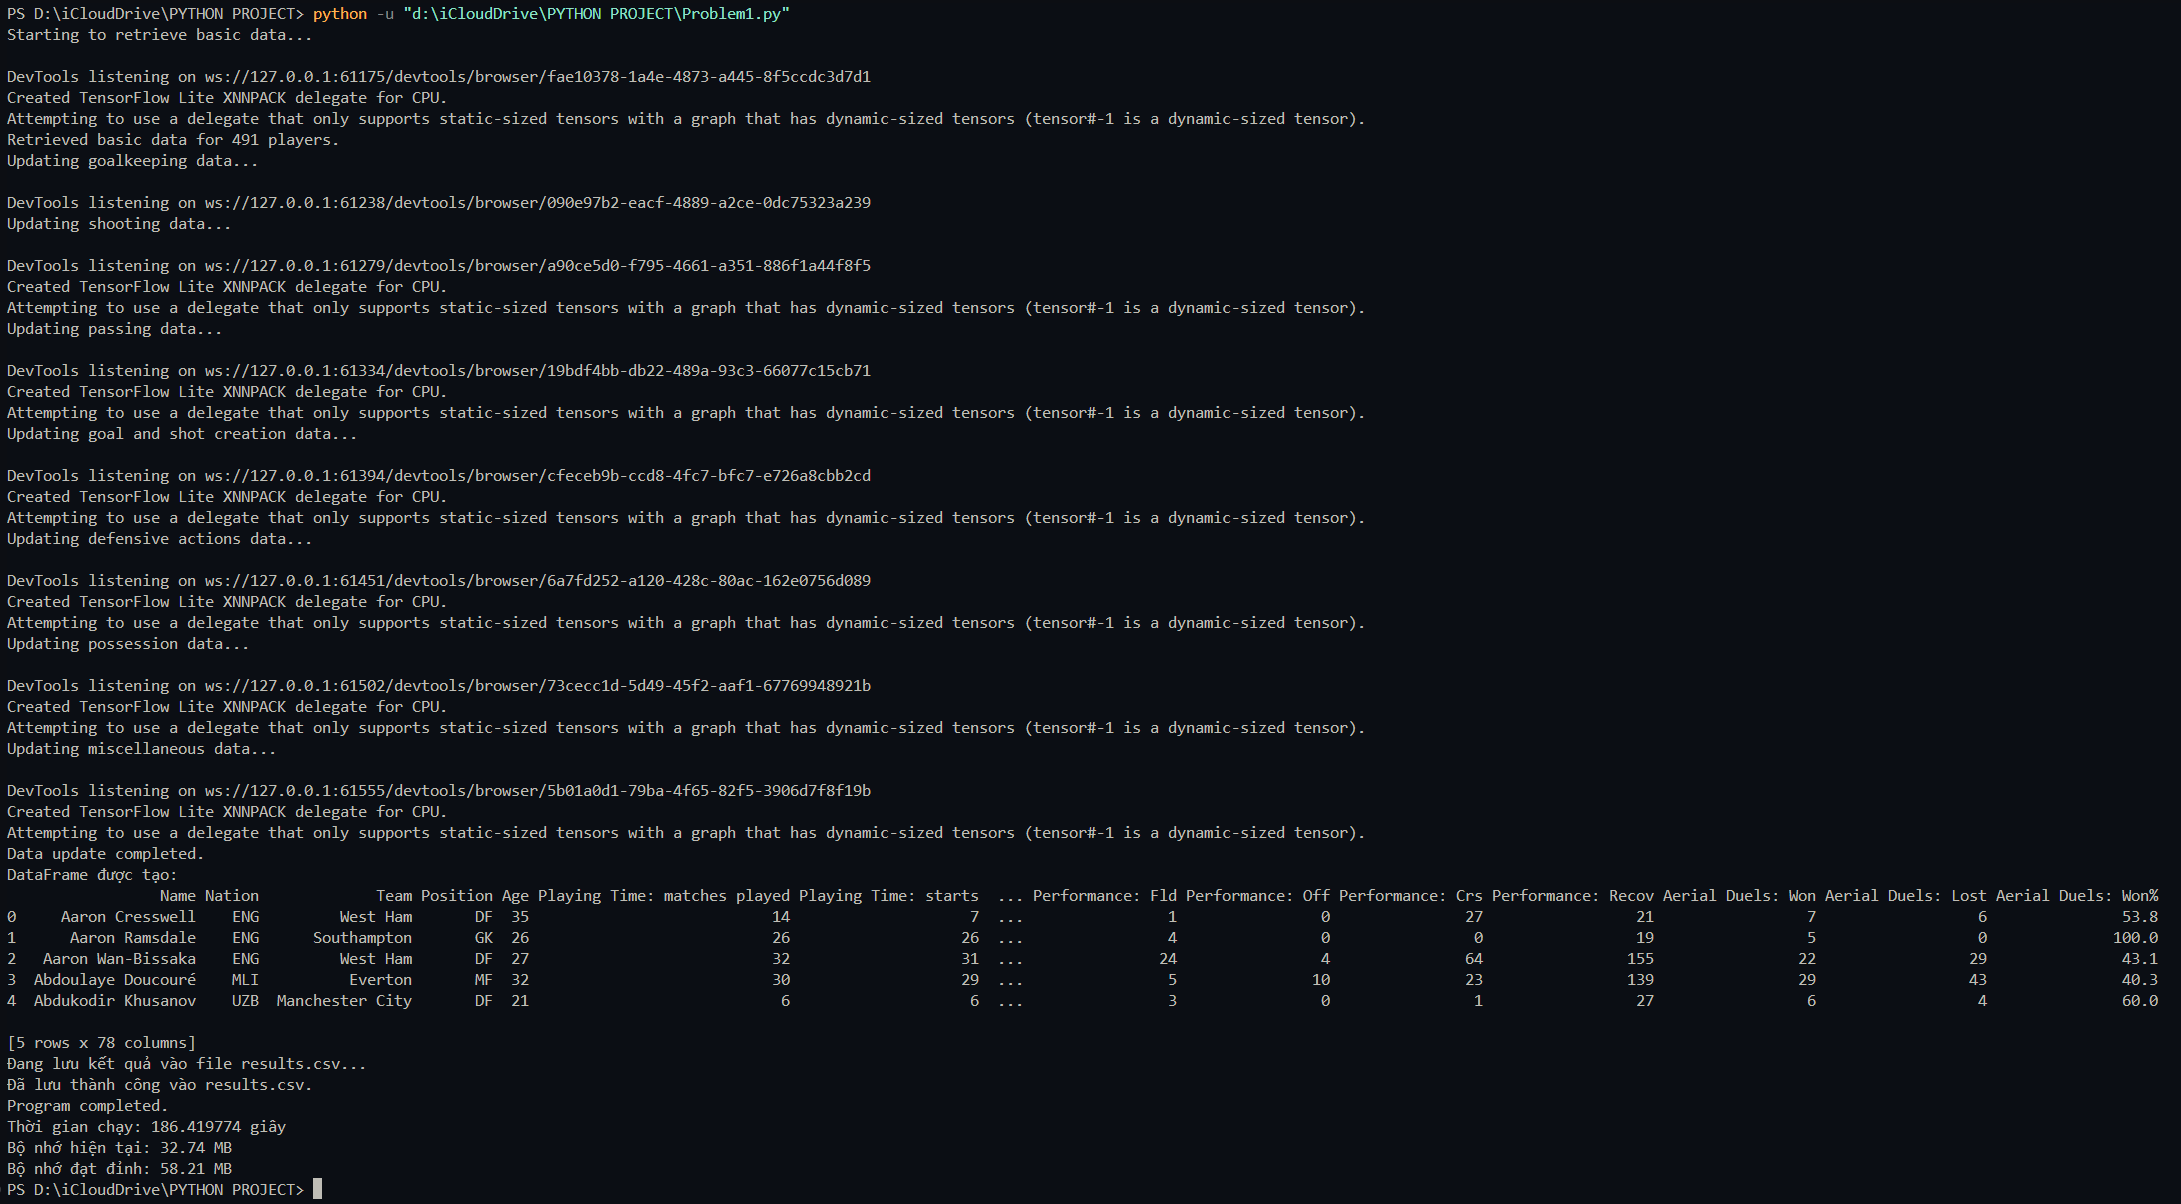
\includegraphics[width=\textwidth]{Terminal.png}
    \caption{Terminal after running the Problem1.py program} % Translated
    \label{fig:terminal}
\end{figure}
Data Collection: The script starts by announcing "Starting to retrieve team data..." and then "Retrieved basic data for 491 players.". Next, it updates various types of data such as performance data, starting lineup data, goal and shot creation data, defensive action data, and possession data.
DevTools Connection: The lines "DevTools listening on ws://127.0.0.1:..." repeat multiple times. This usually appears when a browser automation tool (Selenium) is used, possibly for retrieving data from websites.
Displaying Tabular Data: After data update is completed ("Data update completed."), the script displays a portion of the data table. The table shows the first 5 rows and has a total of 78 columns.
Saving and Ranking Results: The script announces "All data written to the file results.csv." and then "Attempting to rank the results.csv.".
Completion and Execution Time: Finally, the script reports "Process complete." and indicates the execution time was approximately 186.419472 seconds; Maximum memory usage: 32.74 MB; Peak memory: 58.21 MB.

\begin{figure}[h]
    \centering
    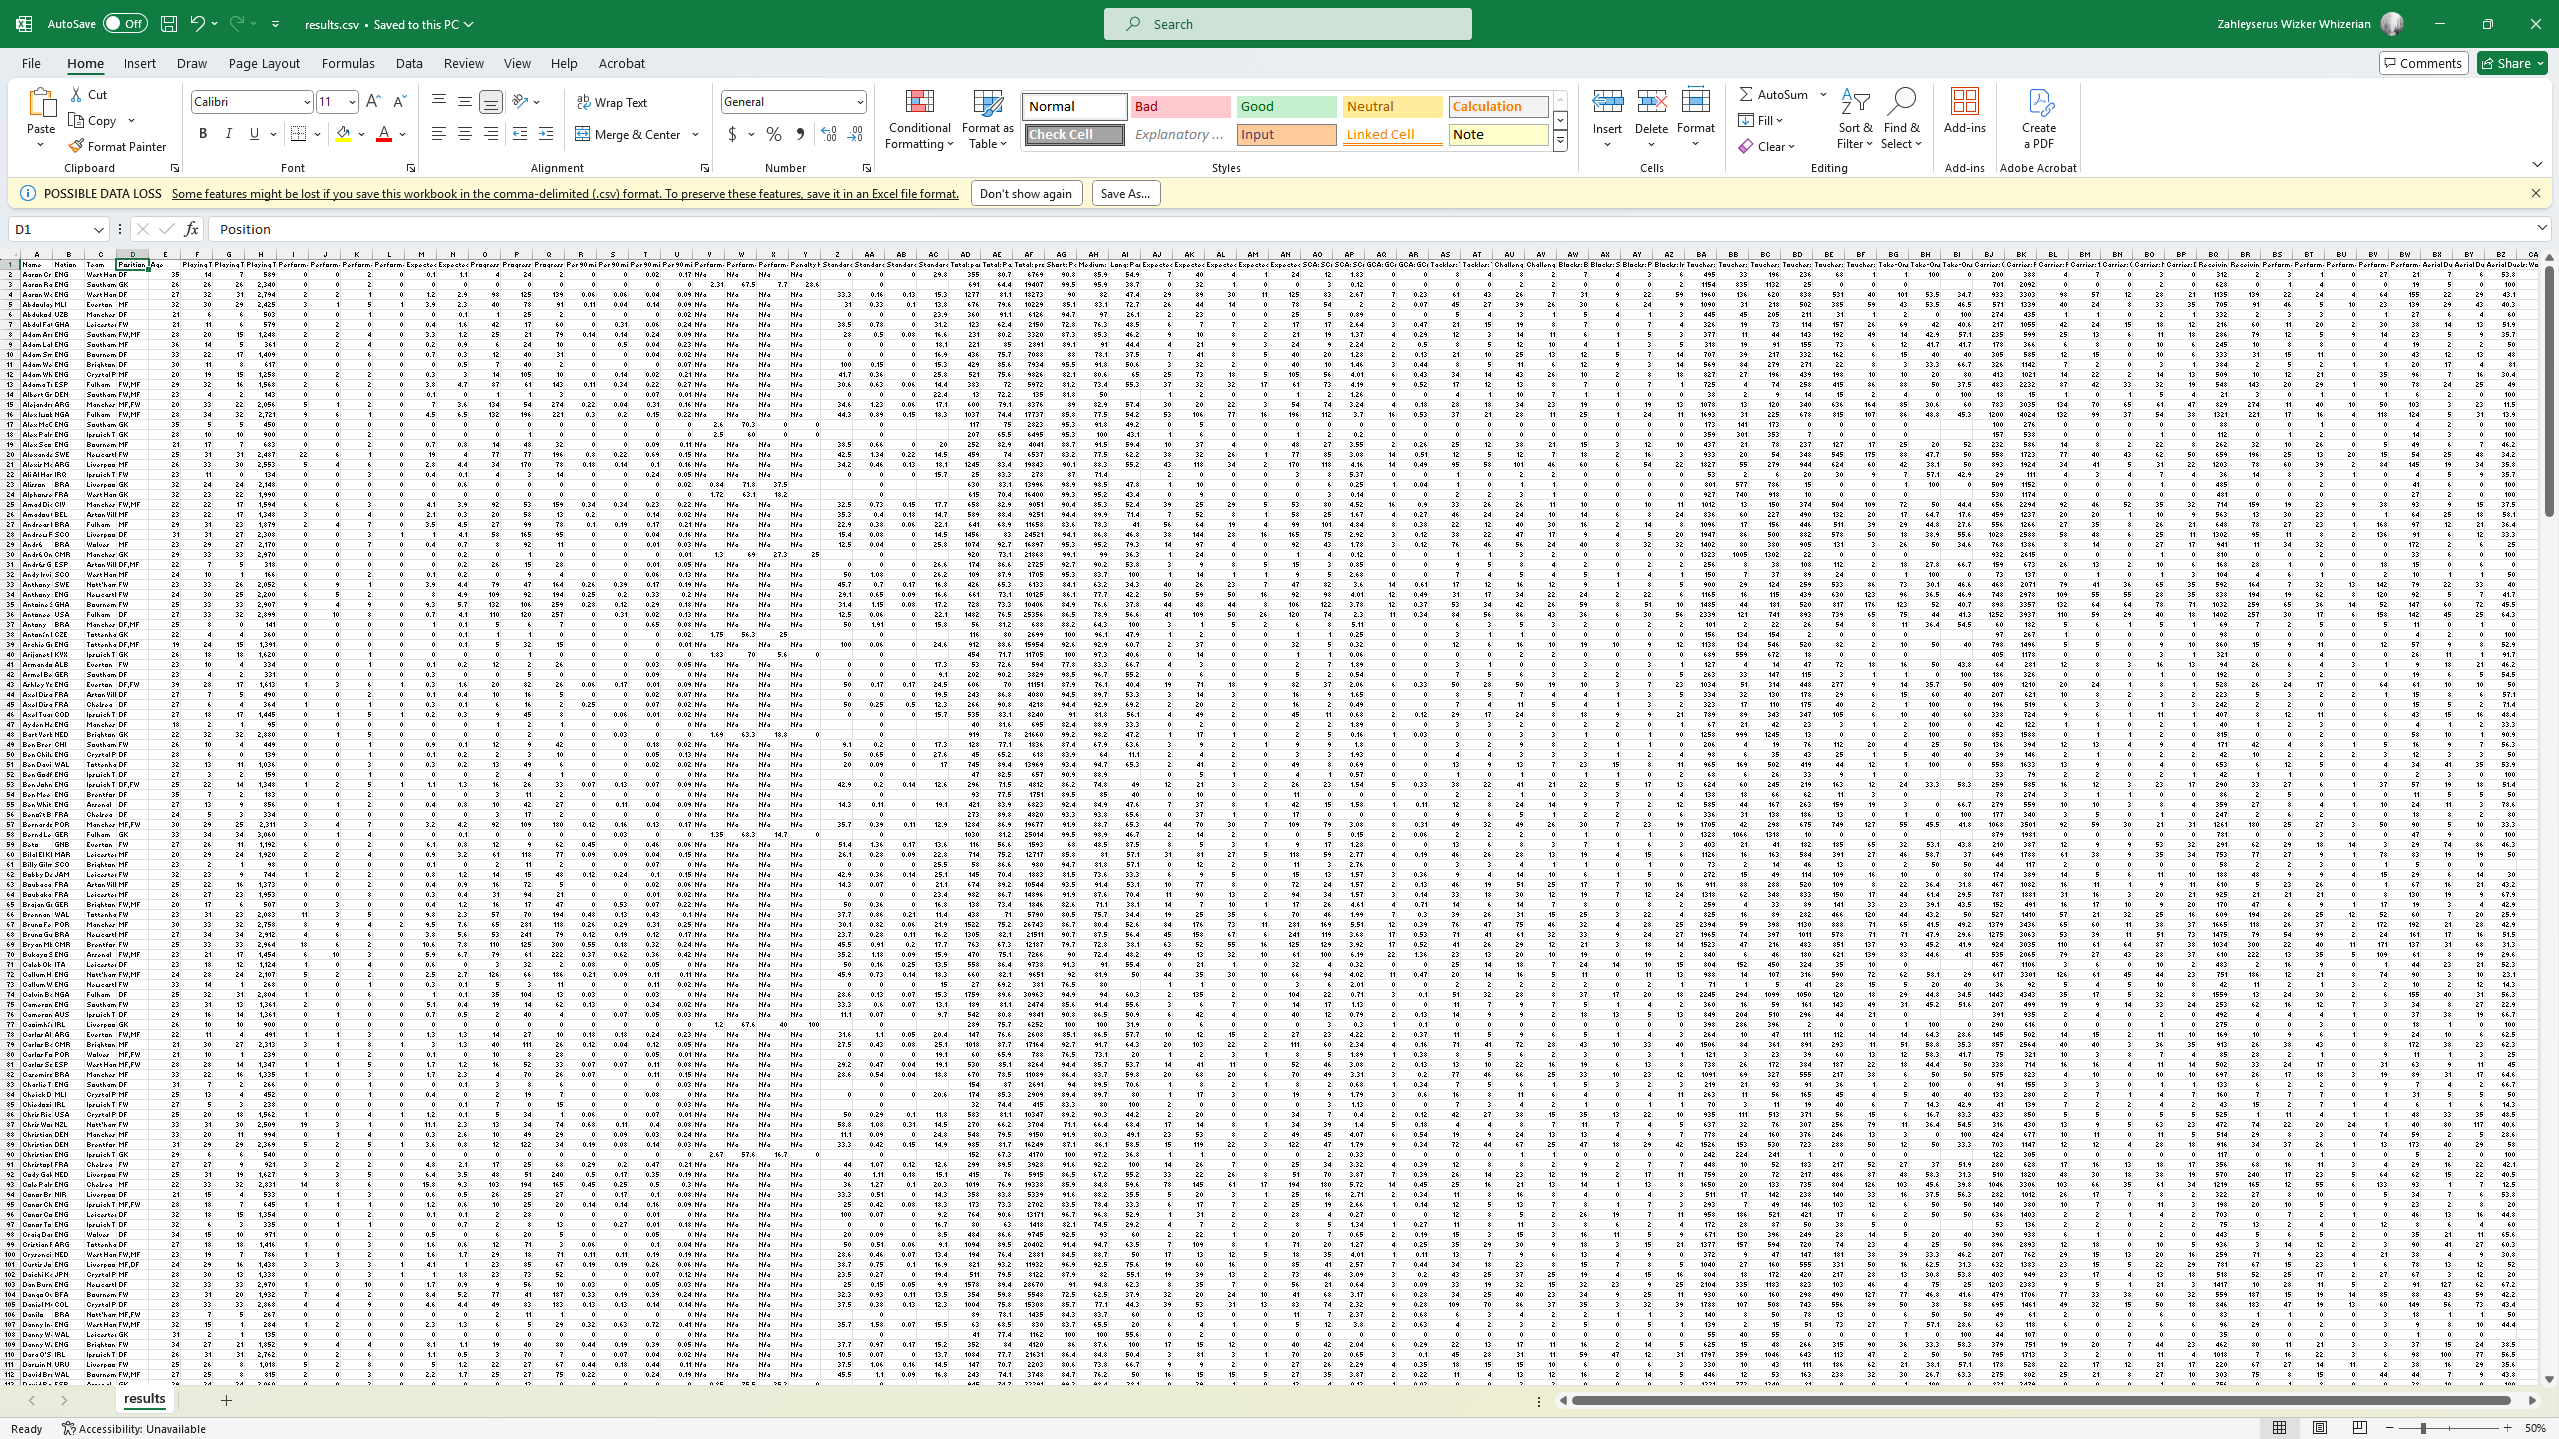
\includegraphics[width=\textwidth]{results_csv.png}
    \caption{File results.csv} % Translated
    \label{fig:terminal} % Note: Label reused, potentially should be unique
\end{figure}
The data file results.csv compiles detailed statistical information for 491 professional football athletes, with each subject described through 78 quantitative and qualitative variables. The data fields include personal information (full name, nationality, current club, playing position, age), playing time information (matches played, starts, total minutes played), performance achievements (goals scored, assists, cards received), along with predictive performance indicators (Expected Goals - xG, Expected Assisted Goals - xAG). Additionally, the dataset provides metrics related to ball control skills, passing, dribbling, defense, ball progression, average performance normalized per 90 minutes of play, as well as aerial duel efficiency.
\subsection{Evaluation:} % Translated
The program in the Problem1.py file implements a process for collecting, consolidating, and exporting detailed statistical data of Premier League players through web scraping techniques, combining Selenium and BeautifulSoup. Data is extracted from multiple specialized statistical tables on fbref.com, including standard stats, goalkeeper stats, shooting ability, passing, possession, defense, and other miscellaneous metrics. Each player is represented as a dictionary with a unique identifier key (combining name and club), ensuring data integrity during updates from multiple sources. After complete collection, the program builds a DataFrame with 78 attributes and exports the results to a standard formatted CSV file, suitable for deeper statistical data analysis. Regarding execution time, the program completes the entire process in approximately 186.4 seconds, demonstrating the ability to collect detailed and accurate data, but with low efficiency. The main reason stems from initiating multiple independent Chrome browser sessions for each type of data table, incurring repeated startup costs, page loading, and browser closing. In terms of memory usage, the program operates efficiently, using a maximum of about 32.74 MB of RAM throughout the collection and processing phase, indicating resourcefulness in memory due to simple data structuring and sequential processing. In summary, the program achieves high accuracy and well-organized data structuring, but has a clear drawback in execution time due to an unoptimized web access process, while its notable advantage is low memory usage, suitable for systems with limited resources.
\clearpage
\chapter{PROBLEM II} % Translated
{
\section{Requirement} % Translated
\begin{itemize}
	\item Identify the top 3 players with the highest and lowest scores for each statistic. Save result to a file named \texttt{top\_3.txt}.
	\item Find the median for each statistic.
Calculate the mean and standard deviation for each statistic across all players and for each team. Save the results to a file named 'results2.csv' with the following format:
	\begin{table}[h]
		\centering
		\begin{tabular}{|c|c|c|c|c|c|}
		\hline
		 &  & Median of Attribute 1 & Mean of Attribute 1 & Std of Attribute 1 & \ldots \\ \hline
		0 & all &  &  &  &  \\ \hline
		1 & Team 1 &  &  &  &  \\ \hline
		\vdots & \vdots &  &  &  &  \\ \hline
		n & Team n &  &  &  &  \\ \hline
		\end{tabular}
		\caption{Statistics per team} % Translated (Original had no text)
	\end{table}
	\item Plot a histogram showing the distribution of each statistic for all players in the league and each team.
	\item Identify the team with the highest scores for each statistic. Based on your analysis, which team do you think is performing the best in the 2024-2025 Premier League season?
\end{itemize}
\section{Implementation Steps} % Translated
\begin{enumerate}
	\item Perform statistical data analysis of football players from the input CSV file (results.csv). First, read the data, process the numerical columns, and divide into qualitative and quantitative information groups.
\item Then, the program proceeds to find the Top 3 players with the highest and lowest scores for each statistic type. Output the results to the top3.txt file as required.
	\item Calculate aggregate statistics such as mean, median, and standard deviation for the entire league as well as for each individual team. These results are saved to the results2.csv file as required by the problem statement.
\item Visualize the data by plotting distribution charts for the metrics, including both overall league charts and detailed charts for each team. These charts are saved as image files.
\item Identify the strongest team based on comparing the average metrics, and compile the team with the most best metrics into "Best Overall Team". This result is also recorded.
\end{enumerate}
\section{Actual Code and Detailed Description} % Translated
\subsection{Main Function} % Translated
\lstset{
    language=Python,
    basicstyle=\ttfamily\scriptsize,
    keywordstyle=\color[rgb]{0.878, 0.467, 0.0}, % dark blue for keyword
    commentstyle=\color[rgb]{0.5,0.5,0.5}, % gray for comment
    stringstyle=\color[rgb]{0, 0.4, 0},
    identifierstyle=\color[rgb]{0.0, 0.298, 0.380}, % normal for variable
    numbers=left,
    numberstyle=\tiny\color[rgb]{0.5,0.5,0.5},
    numbersep=5pt,
    showstringspaces=false,
    breaklines=true,
    tabsize=2
}
\begin{lstlisting}
def Problem_2():
    df, stats_cols, non_numeric_cols = read_data()
 # 1. Find top 3 highest and lowest for each statistic
    Find_Top_3(df, stats_cols)
    # 2. Calculate Median, Mean, Std for each statistic
    Calculate_For_Each_Statistic(df, stats_cols)
    # 3. Plotting
    Plotting(df)
    # 4. Identify the best team for each statistic
    Best_Team_Summary(df, stats_cols)
\end{lstlisting}
\textbf{Operations are performed in the exact sequence described in the implementation steps section:} % Translated

\textbf* {Function read\_data():} Input data: % Translated
\begin{itemize}
	\item Input data from the results.csv file saved in Problem 1 (instead of retrieving data again).
	\item Return DataFrame, Statistics columns, non-numeric columns (analysis data).
\end{itemize}

\textbf* {Function Find\_Top\_3(df, stats\_cols)} % Translated
\begin{itemize}
	\item Input data is DataFrame and statistics columns (Result of function read\_data()).
	\item Perform the search for top 3 (highest and lowest for each metric).
	\item Export data to top\_3.txt file as required.
\end{itemize}

\textbf* {Calculate\_For\_Each\_Statistic(df, stats\_cols)} % Translated
\begin{itemize}
	\item Input data is DataFrame and statistics columns (Result of function read\_data()).
	\item Proceed with steps to derive values for each team (mean, standard deviation) for all fields.
	\item Format into the required fields then fix into a DataFrame.
	\item Export data to 'results2.csv' file as required.
\end{itemize}

\textbf* {Function Plotting(df)} % Translated
\begin{itemize}
	\item Input data is DataFrame (Result of function read\_data()).
	\item Proceed with steps to draw composite graphs. Draw according to the 3 attack metrics, 3 defense metrics. Output the results.
	\item Sequentially draw graphs for each metric, package data by team to create graphs (one graph per team). Output the data.
\end{itemize}

\textbf* {Function Best\_Team\_Summary(df, stats\_cols)} % Translated
\begin{itemize}
	\item Input data is DataFrame and statistics columns (Result of function read\_data()).
	\item Process data, find the team with the highest value for each metric.
	\item Count the number of leading metrics for each team to find the team with the best performance, then make a prediction.
\end{itemize}

\subsection{Detailed Operations} % Translated
\textbf* {Operation read\_data() (Read input data):} % Translated
\lstset{
    language=Python,
    basicstyle=\ttfamily\scriptsize,
    keywordstyle=\color[rgb]{0.878, 0.467, 0.0}, % dark blue for keyword
    commentstyle=\color[rgb]{0.5,0.5,0.5}, % gray for comment
    stringstyle=\color[rgb]{0, 0.4, 0},
    identifierstyle=\color[rgb]{0.0, 0.298, 0.380}, % normal for variable
    numbers=left,
    numberstyle=\tiny\color[rgb]{0.5,0.5,0.5},
    numbersep=5pt,
    showstringspaces=false,
    breaklines=true,
    tabsize=2
}
\begin{lstlisting}
def read_data():
    # Load the data
    df = pd.read_csv('results.csv') # Corrected filename

  # Columns that are not statistics
    non_numeric_cols = ['Name', 'Nation', 'Team', 'Position', 'Age']
    stats_cols = [col for col in df.columns if col not in non_numeric_cols]

    # Clean numeric columns (remove commas and convert to numbers)
    for col in stats_cols:
        if col in df.columns: # Check if column exists
             df[col] = df[col].astype(str).str.replace(',', '', regex=False)
             df[col] = pd.to_numeric(df[col], errors='coerce')

    return df, stats_cols, non_numeric_cols
\end{lstlisting}

In this operation, first, retrieve data from the file: results.csv, create a new DataFrame containing this data [line 3]; Process, separate the data needing statistics (into a list) and data not needing statistics [lines 6, 7]. After basically retrieving the data, continue processing some data regions like numbers with commas, converting them to digits [lines 10 - 12]. Return the results which are the processed DataFrame and lists.

\textbf* {Operation Find\_Top\_3(df, stats\_cols) (Find top 3 players (highest and lowest) for each metric)} % Translated
\lstset{
    language=Python,
    basicstyle=\ttfamily\scriptsize,
    keywordstyle=\color[rgb]{0.878, 0.467, 0.0}, % dark blue for keyword
    commentstyle=\color[rgb]{0.5,0.5,0.5}, % gray for comment
    stringstyle=\color[rgb]{0, 0.4, 0},
    identifierstyle=\color[rgb]{0.0, 0.298, 0.380}, % normal for variable
    numbers=left,
    numberstyle=\tiny\color[rgb]{0.5,0.5,0.5},
    numbersep=5pt,
    showstringspaces=false,
    breaklines=true,
tabsize=2
}
\begin{lstlisting}
def Find_Top_3(df, stats_cols):
    top3_results = []

    for col in stats_cols:
        if col not in df.columns or df[col].dropna().empty: # Check column existence
            continue # Skip empty or non-existent columns

        # Top 3 highest
        top_high = df[['Name', 'Team', col]].sort_values(by=col, ascending=False).head(3)

        # Top 3 lowest
top_low = df[['Name', 'Team', col]].sort_values(by=col, ascending=True).head(3)

        section = f"=== {col} ===\n"
        section += "Top 3 Highest:\n"
        for idx, row in top_high.iterrows():
            section += f"  {row['Name']} ({row['Team']}): {row[col]}\n"

        section += "Top 3 Lowest:\n"
        for idx, row in top_low.iterrows():
           section += f"  {row['Name']} ({row['Team']}): {row[col]}\n"

        section += "\n"
        top3_results.append(section)

    # Save to top_3.txt
    with open('top_3.txt', 'w', encoding='utf-8') as f:
        f.write("\n".join(top3_results))

    print("top_3.txt saved!")
\end{lstlisting}
First, initialize a list to store the output data [line 2]. Start iterating through each column in the list of statistic values. Skip empty columns (Avoid data noise if any) [lines 5, 6]. Create a new DataFrame to store the top 3 of the metric (Highest and lowest) [lines 9, 12]. Lines 14 to 23 are operations to create data for output (write descriptions for easy reading of the output file). In this operation, retrieve player name, team name, and the value in the column being considered. After writing, add it to the list created at the beginning. Continue looping until the end of the table columns. After retrieving all results, write the results to the top\_3.txt file as required [lines 27 - 29].

\textbf* {Operation Calculate\_For\_Each\_Statistic(df, stats\_cols) (Create table summarizing mean, median, std deviation for teams)} % Translated
\lstset{
    language=Python,
    basicstyle=\ttfamily\scriptsize,
    keywordstyle=\color[rgb]{0.878, 0.467, 0.0}, % dark blue for keyword
    commentstyle=\color[rgb]{0.5,0.5,0.5}, % gray for comment
    stringstyle=\color[rgb]{0, 0.4, 0},
    identifierstyle=\color[rgb]{0.0, 0.298, 0.380}, % normal for variable
    numbers=left,
  numberstyle=\tiny\color[rgb]{0.5,0.5,0.5},
    numbersep=5pt,
    showstringspaces=false,
    breaklines=true,
    tabsize=2
}
\begin{lstlisting}
# Helper function to save DataFrame, defined earlier or assumed available
# def save_df_to_file(name, res):
#     results_df = pd.DataFrame(res) # Convert list of dicts to DataFrame
#     results_df.to_csv(name, index=False, encoding='utf-8-sig')

def Calculate_For_Each_Statistic(df, stats_cols):
    # Group by Team + one overall ("all")
    grouped = df.groupby('Team')
    summary_rows = []

    # First row: "all" players
    summary_all = {'Team': 'all'}
    for col in stats_cols:
        if col in df.columns: # Check column existence
            summary_all[f'Median of {col}'] = df[col].median()
            summary_all[f'Mean of {col}'] = df[col].mean()
     summary_all[f'Std of {col}'] = df[col].std()
    summary_rows.append(summary_all)

    # Each team's stats
    for team, team_df in grouped:
        summary_team = {'Team': team}
        for col in stats_cols:
             if col in team_df.columns: # Check column existence
                summary_team[f'Median of {col}'] = team_df[col].median()
                summary_team[f'Mean of {col}'] = team_df[col].mean()
                summary_team[f'Std of {col}'] = team_df[col].std()
      summary_rows.append(summary_team)

    # Save to results2.csv
    results_df = pd.DataFrame(summary_rows) # Create DataFrame here
    results_df.to_csv('results2.csv', index=False, encoding='utf-8-sig')
    # save_df_to_file('results2.csv', summary_rows) # Assumes helper function exists
    print("results2.csv saved!")
\end{lstlisting}

Initialize necessary components for data processing: Create a DataFrame grouped by teams [line 8]; Create a list to store values row by row [line 9]. Process values in the first row (all) by looping through each column of the statistics table to derive the 3 required values [Lines 12 - 17]. Process data for each team row. Perform a loop to find data for each team. Continue with another loop for each data field to derive the 3 required metrics for each field and add them to the result storage list. Repeat until all teams are processed [Lines 20 - 26]. Output the data to the results2.csv file using the assumed `save\_df\_to\_file(name, res)` function or direct `to\_csv` call.

\textbf* {Operation Plotting(df) (Create charts)} % Translated
\lstset{
    language=Python,
    basicstyle=\ttfamily\scriptsize,
    keywordstyle=\color[rgb]{0.878, 0.467, 0.0}, % dark blue for keyword
    commentstyle=\color[rgb]{0.5,0.5,0.5}, % gray for comment
    stringstyle=\color[rgb]{0, 0.4, 0},
    identifierstyle=\color[rgb]{0.0, 0.298, 0.380}, % normal for variable
    numbers=left,
    numberstyle=\tiny\color[rgb]{0.5,0.5,0.5},
    numbersep=5pt,
    showstringspaces=false,
    breaklines=true,
    tabsize=2
}
\begin{lstlisting}
# Assume necessary imports like matplotlib.pyplot as plt, seaborn as sns, os, pandas as pd
import matplotlib.pyplot as plt
import seaborn as sns
import os
import pandas as pd

def
Plotting(df):
    # --- Setting up ---
    attack_indexes = [
        'Performance: goals',
        'Performance: assists',
        'Expected: expected goals (xG)'
    ]

    defense_indexes = [
        'Tackles: Tkl',
        'Challenges: Att',
        'Blocks: Blocks'
    ]

    team_column_name = 'Team'
  max_teams_per_row_facet = 4 # How many team plots per row in FacetGrid
    all_indexes = attack_indexes + defense_indexes
    valid_indexes = []

    for col in all_indexes:
        if col in df.columns:
            # Ensure conversion to numeric happens before checking dtype
            df[col] = pd.to_numeric(df[col], errors='coerce')
            if not df[col].isnull().all() and pd.api.types.is_numeric_dtype(df[col]):
                valid_indexes.append(col)
        else:
             print(f"Warning: Column '{col}' not found in DataFrame.")


    # Create output directory if it doesn't exist
    output_dir = 'P2_RES'
    if not os.path.exists(output_dir):
        os.makedirs(output_dir)

    # --- Plotting ---
   # 1. Histograms for the Entire League
    if valid_indexes: # Only plot if there are valid columns
        Histograms_Entire_League(df, valid_indexes, output_dir)

    # 2. Histograms per Team (using FacetGrid)
    if valid_indexes and team_column_name in df.columns: # Ensure team column exists
        Histograms_per_Team(df, team_column_name, valid_indexes, max_teams_per_row_facet, output_dir)

    print("\n--- Plotting Complete ---")

# --- Helper Plotting Functions ---

def Histograms_Entire_League(df, valid_indexes, output_dir):
    print("\n--- Plotting Overall League Distributions ---")
    num_valid_indexes = len(valid_indexes)
    # Calculate grid size for overall plots (e.g., 2 columns)
    ncols_overall = 2
    nrows_overall = (num_valid_indexes + ncols_overall - 1) // ncols_overall

    plt.figure(figsize=(12, 5 * nrows_overall))
    plt.suptitle('Overall League Distribution of Player Indexes', fontsize=16, y=1.02) # Add space with y

    for i, index_col in enumerate(valid_indexes):
     plt.subplot(nrows_overall, ncols_overall, i + 1)
        # Filter out NaN values for plotting if you didn't fill them earlier
        data_to_plot = df[index_col].dropna()
        if not data_to_plot.empty:
            sns.histplot(data_to_plot, kde=True, bins=20)
            plt.title(f'Distribution of {index_col}')
            plt.xlabel(index_col)
 plt.ylabel('Frequency')
        else:
            plt.title(f'{index_col}\n(No valid data to plot)')

    plt.tight_layout(rect=[0, 0, 1, 0.98]) # Adjust layout to prevent overlap with suptitle
    plt.savefig(os.path.join(output_dir, 'Overall_League_Distribution_of_Player_Indexes.png'))
    plt.close() # Close the figure to free memory
    print("\n--- Done Plotting Overall League Distributions ---")


def Histograms_per_Team(df, team_column_name, valid_indexes, max_teams_per_row_facet, output_dir):
    print("\n--- Plotting Per-Team Distributions ---")

    # Check number of unique teams to avoid overly large grids
    if team_column_name not in df.columns:
        print(f"Error: Team column '{team_column_name}' not found.")
        return

    unique_teams = df[team_column_name].nunique()
    print(f"Found {unique_teams} unique teams.")
    if unique_teams > 50: # Add a threshold to prevent overwhelming plots
        print("Warning: High number of teams detected. FacetGrid might be very large.")
       # Optional: Add logic here to maybe plot only a subset of teams or ask user

    for index_col in valid_indexes:
        print(f"Generating FacetGrid for: {index_col}")

        # Filter out NaNs for this specific index and the team column before creating the grid
        facet_data = df[[index_col, team_column_name]].dropna()

        if facet_data.empty or facet_data[index_col].isnull().all():
  print(f"  Skipping {index_col} - No valid data after dropping NaNs.")
            continue

        # Create the FacetGrid
        # Ensure unique_teams is at least 1 for col_wrap
        effective_col_wrap = min(max_teams_per_row_facet, max(1, unique_teams))

        g = sns.FacetGrid(
            facet_data,
            col=team_column_name,
            col_wrap=effective_col_wrap, # Don't wrap more than teams exist or max specified
 sharex=True, # Keep x-axis consistent for comparison
            sharey=False, # Allow y-axis (frequency) to vary per team
            height=3,    # Adjust height of each subplot
            aspect=1.2   # Adjust aspect ratio of each subplot
        )

        # Map the histogram plot onto the grid
g.map(sns.histplot, index_col, kde=True, bins=15) # Use fewer bins for smaller plots

        # Add titles and adjust layout
        g.set_titles("Team: {col_name}")
        # Corrected: Use index_col directly, it's already a string
        g.fig.suptitle(f'Distribution of {index_col} by Team', fontsize=14, y=1.03) # Add overall title slightly above
        g.fig.tight_layout(rect=[0, 0, 1, 0.97]) # Adjust layout
        # Sanitize filename
        safe_col_name = "".join(c if c.isalnum() else "_" for c in index_col)
        plt.savefig(os.path.join(output_dir,'Distribution_of_'+safe_col_name+'_by_Team.png'))
        plt.close() # Close the figure
    print("\n--- Done Plotting Per-Team Distributions ---")

\end{lstlisting}
This function includes 2 main operations: Preparation (coded entirely within the function); Plotting charts (in 2 called sub-functions). Let's go into detail:
\textbf{Setting Up:}\
Initialize the values that will be used for data retrieval to plot charts [Lines 3 - 15] (Including 6 attributes: 3 for attack, 3 for defense). Continue initializing some necessary values to serve the data processing and chart plotting process [lines 15 - 18]. Perform a loop to convert data to numeric format while removing attributes that cannot be statistically analyzed (Ensuring no errors during execution).
\textbf{Plotting:} The operation is performed through 2 sub-programs:
\textbf* {Histograms\_Entire\_League(df, valid\_indexes) Composite chart: } % Translated
\begin{lstlisting}
# Code is included in the listing above
\end{lstlisting}
First, the function receives input and initializes some values to serve the layout arrangement (inputting the number of charts [line 3]; initializing parameters to arrange the figure with 2 charts per row [lines 5, 6]). Line 8 proceeds to create the chart size, default is 12 x 5*(number of chart rows). Create the image name in line 9. Proceed to loop to draw charts for each type of metric input. Line 12 aims to place the chart in the correct pre-arranged position. Line 14 aims to filter out invalid values, e.g., \texttt{'N/a'}. If there are values, proceed to draw the chart, otherwise create an empty cell with the name format as in line 21.

While creating the chart, we use the command:
`sns.histplot(data\_to\_plot, kde=True, bins=20)`
to draw a histogram (frequency chart) of the data in \texttt{data\_to\_plot}.
\begin{itemize}
    \item \texttt{data\_to\_plot}: the data you want to plot the histogram for, can be a list, NumPy array, Pandas Series, etc.
\item \texttt{bins=20}: divides the data into 20 intervals (bins) to draw the histogram. Each bar in the chart represents the number of elements falling within a certain interval.
\item \texttt{kde=True}: draws an additional kernel density estimate (KDE) line – a smooth curve estimating the probability distribution of the data, helping you see the distribution shape (e.g., normal, left-skewed, right-skewed, etc.).
\end{itemize}
After looping through all metrics, fix the layout and save the image [lines 23, 24].
\textbf* { Histograms\_per\_Team(df, team\_column\_name, valid\_indexes, max\_teams\_per\_row\_facet)) Chart by each metric for each team: } % Translated
\begin{lstlisting}
# Code is included in the main Plotting function listing
\end{lstlisting}
\begin{itemize}
\item Initially, the function prints a message indicating the start of the chart plotting process and determines the number of different teams in the input data. If the number of teams is too large, the program issues a warning about the risk of overwhelming the chart display (lines 5–8).
\item Then, the function iterates through each metric in the \texttt{valid\_indexes} list. For each metric, the data is filtered to retain only valid values corresponding to the metric and team name (lines 11–12). If all data for that metric is missing (\texttt{NaN}), the metric is skipped (lines 17–18).
\item For metrics with valid data, the function creates a chart grid (\texttt{FacetGrid}) where each cell represents the distribution of the metric for each team. The grid is adjusted with appropriate height, ratio, and number of columns, while keeping the horizontal axis fixed across charts for easy comparison (lines 22–30).
\item A histogram chart with 15 intervals (\texttt{bins}) along with a KDE density line is mapped onto each cell in the grid (line 33). Each cell has a sub-title showing the team name, while a general title for the entire grid is added at the top. The function uses \texttt{tight\_layout()} to adjust the layout to avoid overlaps (lines 36–38).
\item Finally, the chart is saved to the \texttt{P2\_RES} directory with a dynamic file name based on the metric being processed (line 40), and a message confirming the end of the plotting process is printed (line 41).
\end{itemize}
\textbf* {Operation Best\_Team\_Summary(df, stats\_cols): Find the best team for each metric and predict the team with the best performance} % Translated
\lstset{
    language=Python,
    basicstyle=\ttfamily\scriptsize,
    keywordstyle=\color[rgb]{0.878, 0.467, 0.0}, % dark blue for keyword
    commentstyle=\color[rgb]{0.5,0.5,0.5}, % gray for comment
    stringstyle=\color[rgb]{0, 0.4, 0},
    identifierstyle=\color[rgb]{0.0, 0.298, 0.380}, % normal for variable
    numbers=left,
    numberstyle=\tiny\color[rgb]{0.5,0.5,0.5},
    numbersep=5pt,
    showstringspaces=false,
    breaklines=true,
    tabsize=2
}
\begin{lstlisting}
# Assume necessary imports: os, pandas as pd, collections.Counter
import os
import pandas as pd
from collections import Counter

def Best_Team_Summary(df, stats_cols):
    output_dir = 'P2_RES' # Define output directory
    if not os.path.exists(output_dir):
        os.makedirs(output_dir)

 # Group by Team
    # Ensure 'Team' column exists
    if 'Team' not in df.columns:
        print("Error: 'Team' column not found in DataFrame.")
        return

    grouped_team = df.groupby('Team')

    # Store the best team per stat
    best_team_per_stat = {}

    for col in stats_cols:
        # Ensure column exists and is numeric before processing
        if col not in df.columns or not pd.api.types.is_numeric_dtype(df[col]):
            # print(f"Skipping non-numeric or non-existent column: {col}") # Optional: for debugging
            continue
        if df[col].dropna().empty:
            continue
        # Calculate mean per team
        try:
            mean_per_team = grouped_team[col].mean()
            # Handle cases where all values in a group might be NaN after grouping
            if mean_per_team.isnull().all():
                continue
            best_team_index = mean_per_team.idxmax() # Index (Team name) with highest mean
            best_score = mean_per_team.max()
            best_team_per_stat[col] = (best_team_index, best_score)
        except TypeError as e:
             print(f"Could not calculate mean for {col}: {e}") # Handle potential errors during mean calculation

# best_score = mean_per_team.max() # Moved inside try block
        # best_team_per_stat[col] = (best_team, best_score) # Moved inside try block

    # Count how many times each team was best
    # from collections import Counter # Moved import to top
    if not best_team_per_stat:
         print("No statistics found to determine the best team.")
         return

    team_counter = Counter([team for team, score in best_team_per_stat.values()])

    # Find the team that was best most often
    if not team_counter:
        print("Could not determine the best overall team.")
        return
    best_overall_team, count = team_counter.most_common(1)[0]


    # Save results
    file_path = os.path.join(output_dir, 'best_team_summary.txt')
    data = []

    for stat, (team, score) in best_team_per_stat.items():
        data.append({
          'Statistic': stat,
            'Best Team': team,
            # Ensure score is not NaN before rounding
            'Average Score': round(score, 2) if pd.notna(score) else 'N/A'
        })

    summary_df = pd.DataFrame(data) # Renamed to avoid conflict

    overall_row = {
        'Statistic': 'Best Overall Team',
        'Best Team': best_overall_team,
        'Average Score': f'Top in {count} statistics'
    }

  # Use concat instead of append (append is deprecated)
    summary_df = pd.concat([summary_df, pd.DataFrame([overall_row])], ignore_index=True)
    summary_df.to_csv(file_path, index=False, sep='\t') # Use summary_df here
    print(f"Best team identified: {best_overall_team} (Top in {count} stats).")
# print(f"See '{file_path}'.") # More informative path
\end{lstlisting}
\begin{itemize}
    \item First, the data is grouped by the \texttt{'Team'} column to facilitate calculating the average value for each team (line 3). A dictionary \texttt{best\_team\_per\_stat} is initialized to store the team with the highest score for each metric (line 6).

    \item The function then iterates through each metric in the \texttt{stats\_cols} list. If a column contains only missing values (\texttt{NaN}), that metric is skipped (lines 9--10). For each valid metric, the average value per team is calculated, and the team with the highest average value is identified using the \texttt{idxmax()} method (lines 12--14). The pair of information including the team name and the average value is stored in the result dictionary (line 15).

    \item Next, the function uses \texttt{collections.Counter} to count the number of times each team was selected as the best team across the metrics (lines 18--18). The team considered the overall leader is the one that appears most frequently in these selections (line 22).

    \item Then, the results are prepared for writing to a text file. A list \texttt{data} is created, where each element is a row containing the metric name, the leading team's name, and the average score (lines 25--35). A summary row (\texttt{overall\_row}) is added, recording the overall leading team along with the number of metrics that team leads (lines 37--41).
\item Finally, all the information is packaged into a \texttt{DataFrame} and exported to the file \texttt{best\_team\_summary.txt} in TSV format (tab-separated values) within the \texttt{P2\_RES} directory (lines 43--44). A confirmation message is printed to the screen to confirm the completion of the processing (line 45).
\end{itemize}
\section{Results and Evaluation} % Translated
\subsection{Results} % Translated
\subsubsection{General Results} % Translated
\begin{figure}[h]
    \centering
    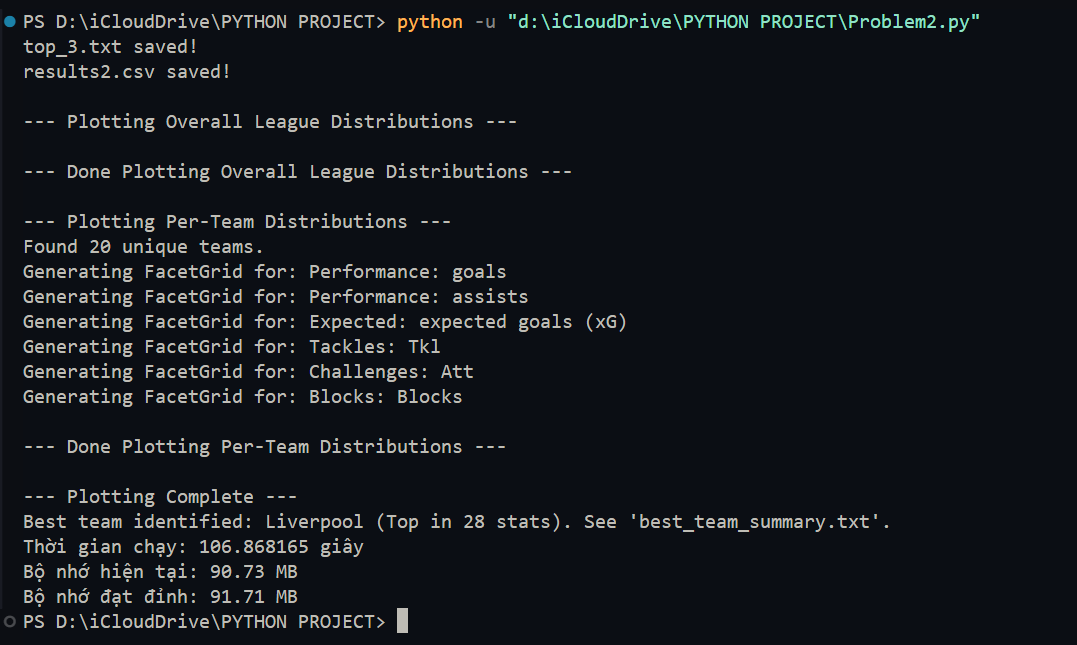
\includegraphics[width=300px]{Terminal_2.png}
    \caption{Terminal after running the Problem2.py program} % Translated
    \label{fig:terminal2}
\end{figure}
The terminal snippet shows the successful execution of the Python script \texttt{Problem2.py}. During execution, the program saved two result files, \texttt{top\_3.txt} and \texttt{results2.csv}, then proceeded to plot data distribution charts for the entire league and for each team. A total of 20 teams were identified, and charts were generated for multiple metrics such as \texttt{goals}, \texttt{assists}, \texttt{expected goals (xG)}, \texttt{tackles (Tkl)}, \texttt{challenges (Att)}, and \texttt{blocks}. The analysis result indicates that \texttt{Liverpool} is the best-performing team, leading in 28 metrics. Detailed information is saved in the file \texttt{best\_team\_summary.txt}. The process completed in approximately 106.87 seconds with a maximum memory usage of 91.71 MB.

\begin{figure}[h]
    \centering
    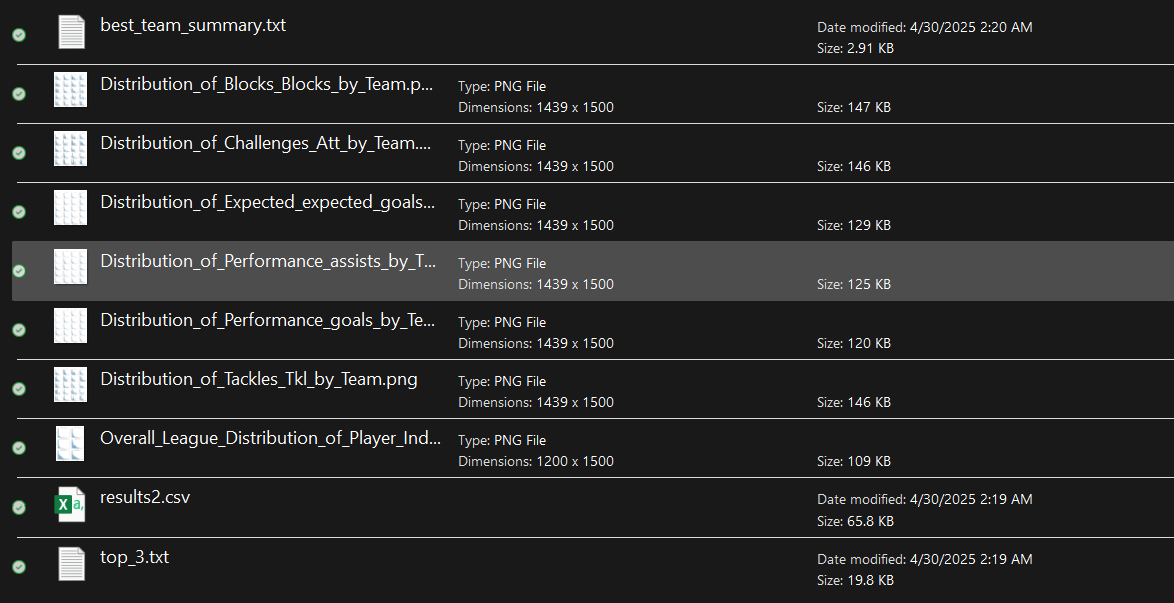
\includegraphics[width=300px]{P2_RES.png}
    \caption{Output files after running the Problem2.py program} % Translated
    \label{fig:output}
\end{figure}
The program output consists of 10 files, including 2 .txt files, 1 .csv file, and 7 .png files. The top\_3.txt file contains the output data of the function finding the top 3 highest and lowest players for each metric. The results2.csv file is the output of the function summarizing the mean, median, and standard deviation for each team according to the output requirements. The .png files include 1 image consolidating 6 attributes of all players containing 6 charts, and the remaining 6 images each contain 20 charts, which are statistics according to the 6 attributes for each team. This is also the output result of the chart plotting program. The final txt file is the output result of the program finding the team with the highest value in each attribute and predicting the team with the best performance of the season.
\subsubsection{Detailed Output Results} % Translated
\textbf{top\_3.txt} % Translated
This file provides a detailed quantitative analysis of player performance in a football league, sorted by statistical categories. Each category compares the "Top 3 Highest" and "Top 3 Lowest" to highlight the performance range. Categories include playing time, performance (e.g., goals, assists), expected stats (e.g., xG, xAG), progression stats, per 90 minutes stats, standard stats, passing stats, key passes, shot-creating actions, tackles and challenges, interceptions and blocks, touches, dribbling, passing, receiving, and fouls. Overall, the file offers a structured view of player strengths and weaknesses.
\begin{figure}[h]
    \centering
    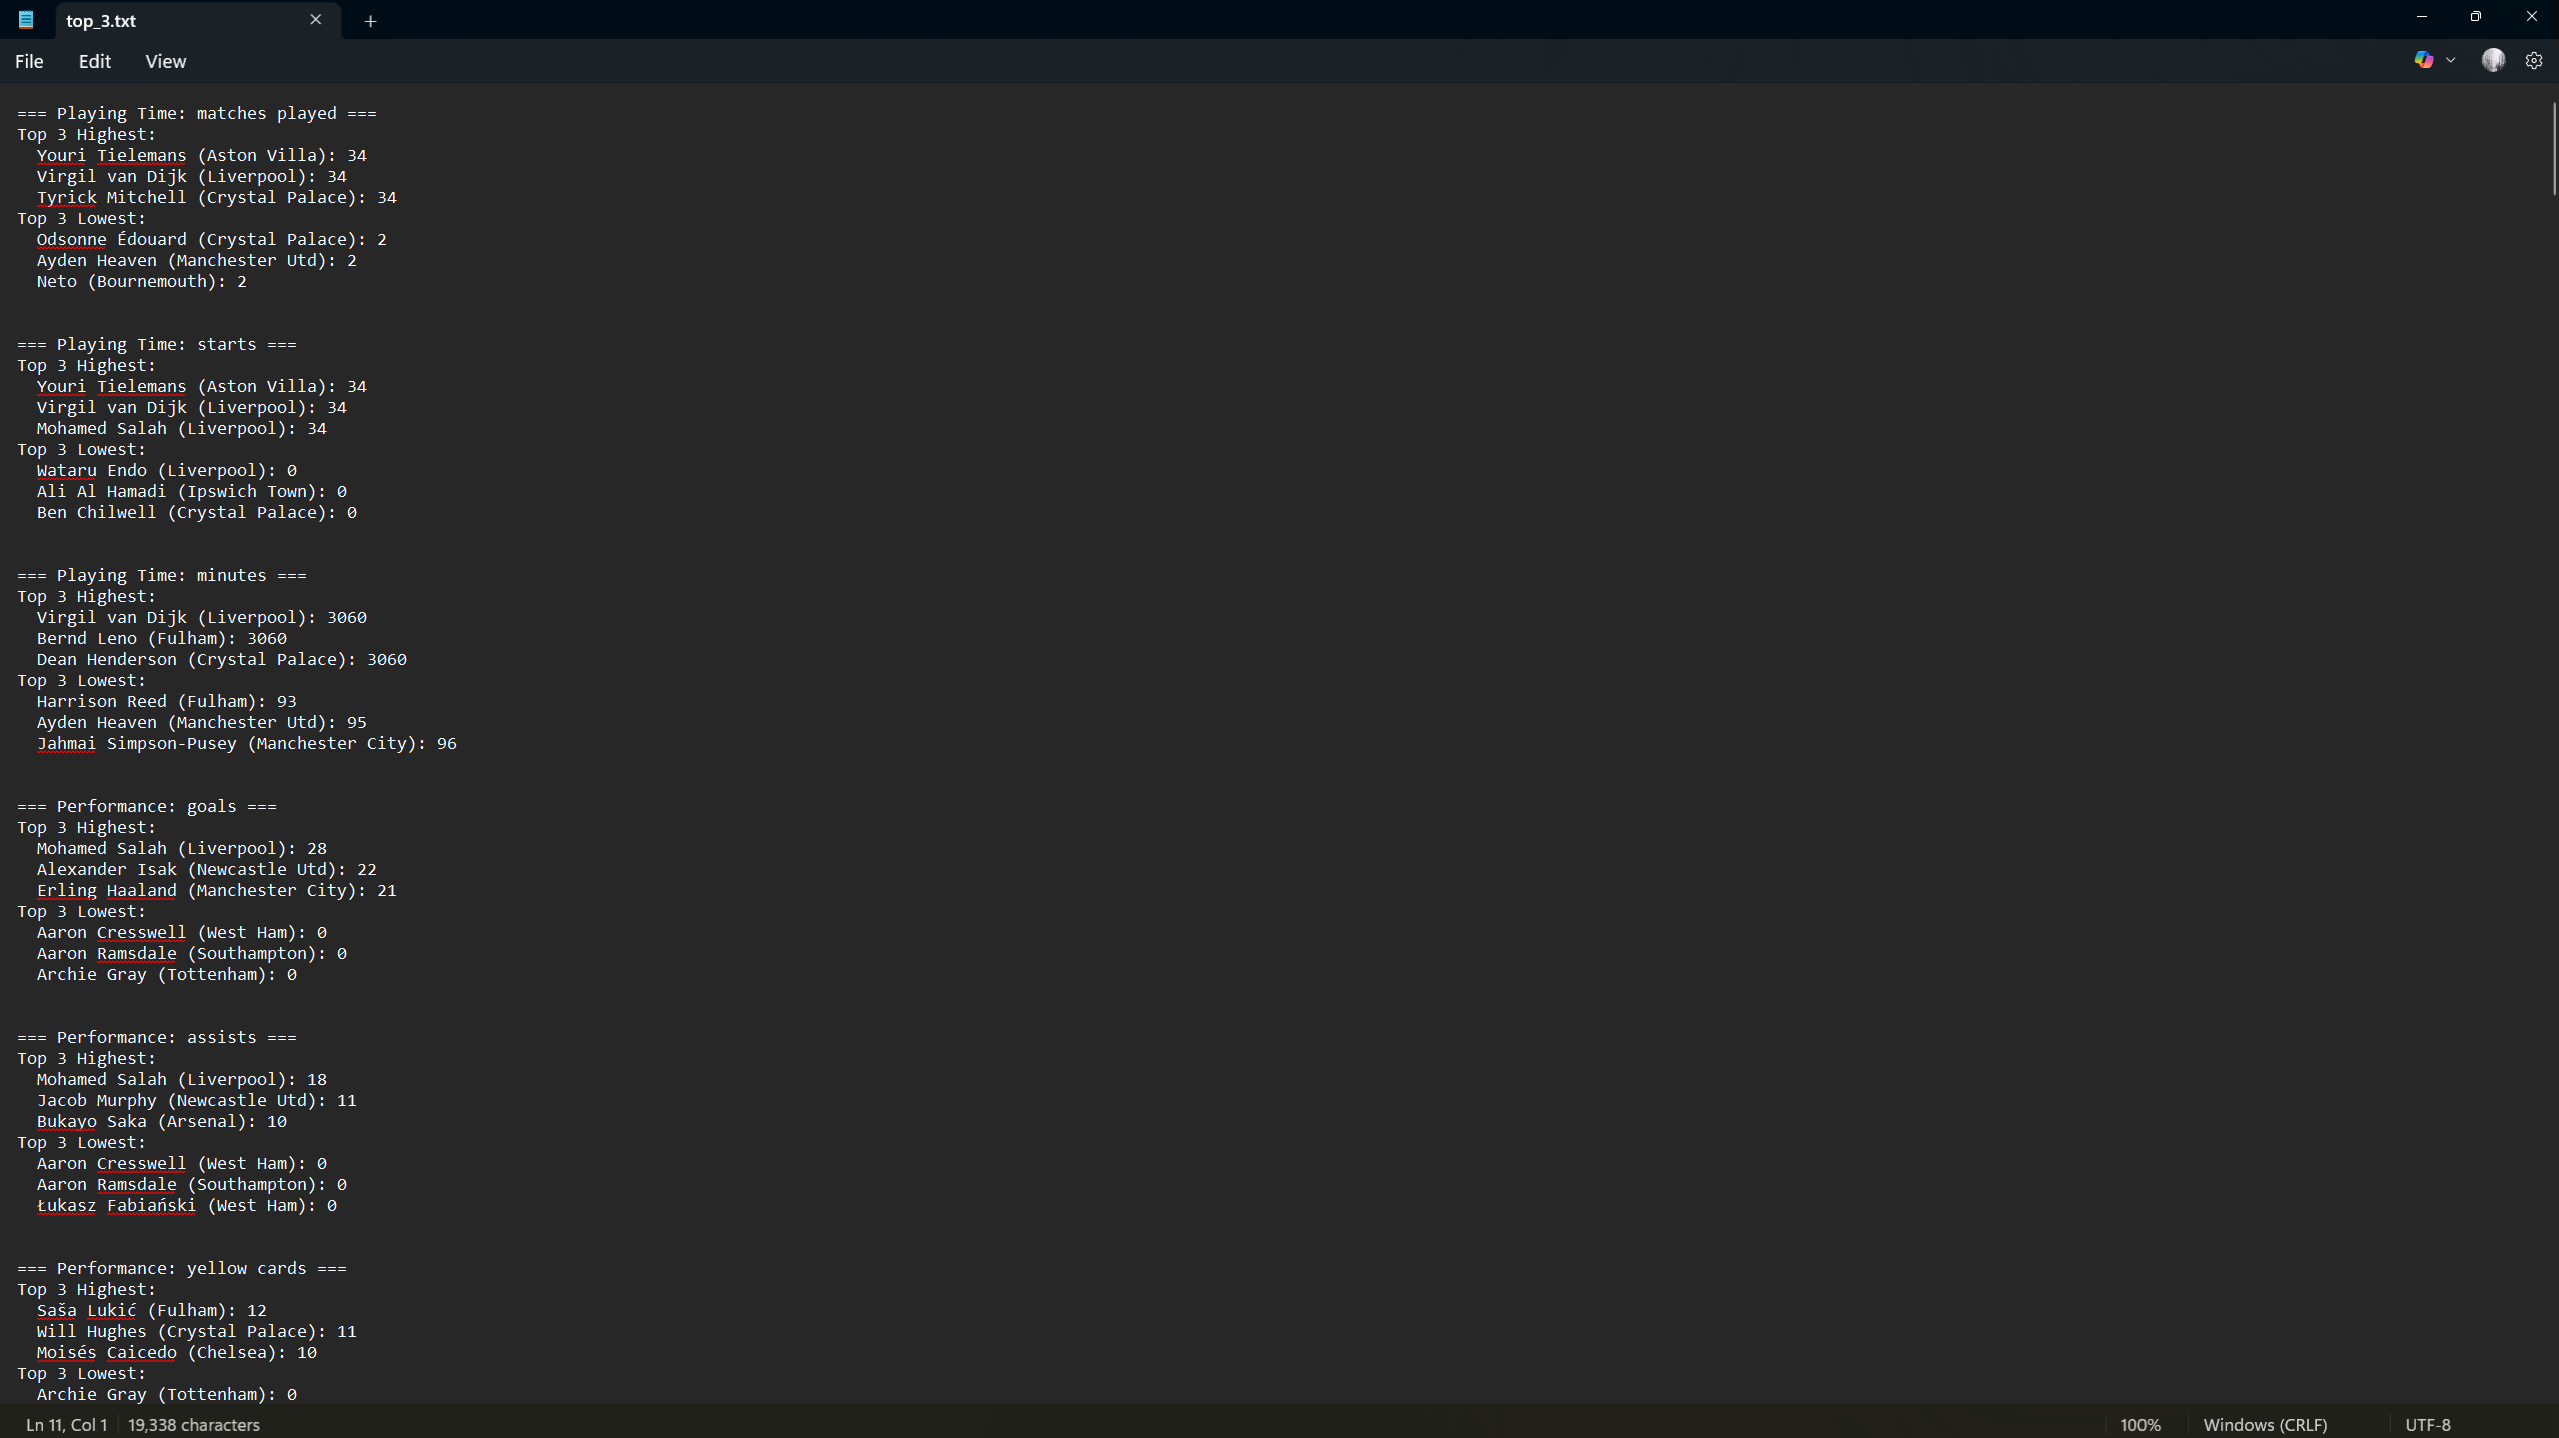
\includegraphics[width=220px]{top_3.png}
    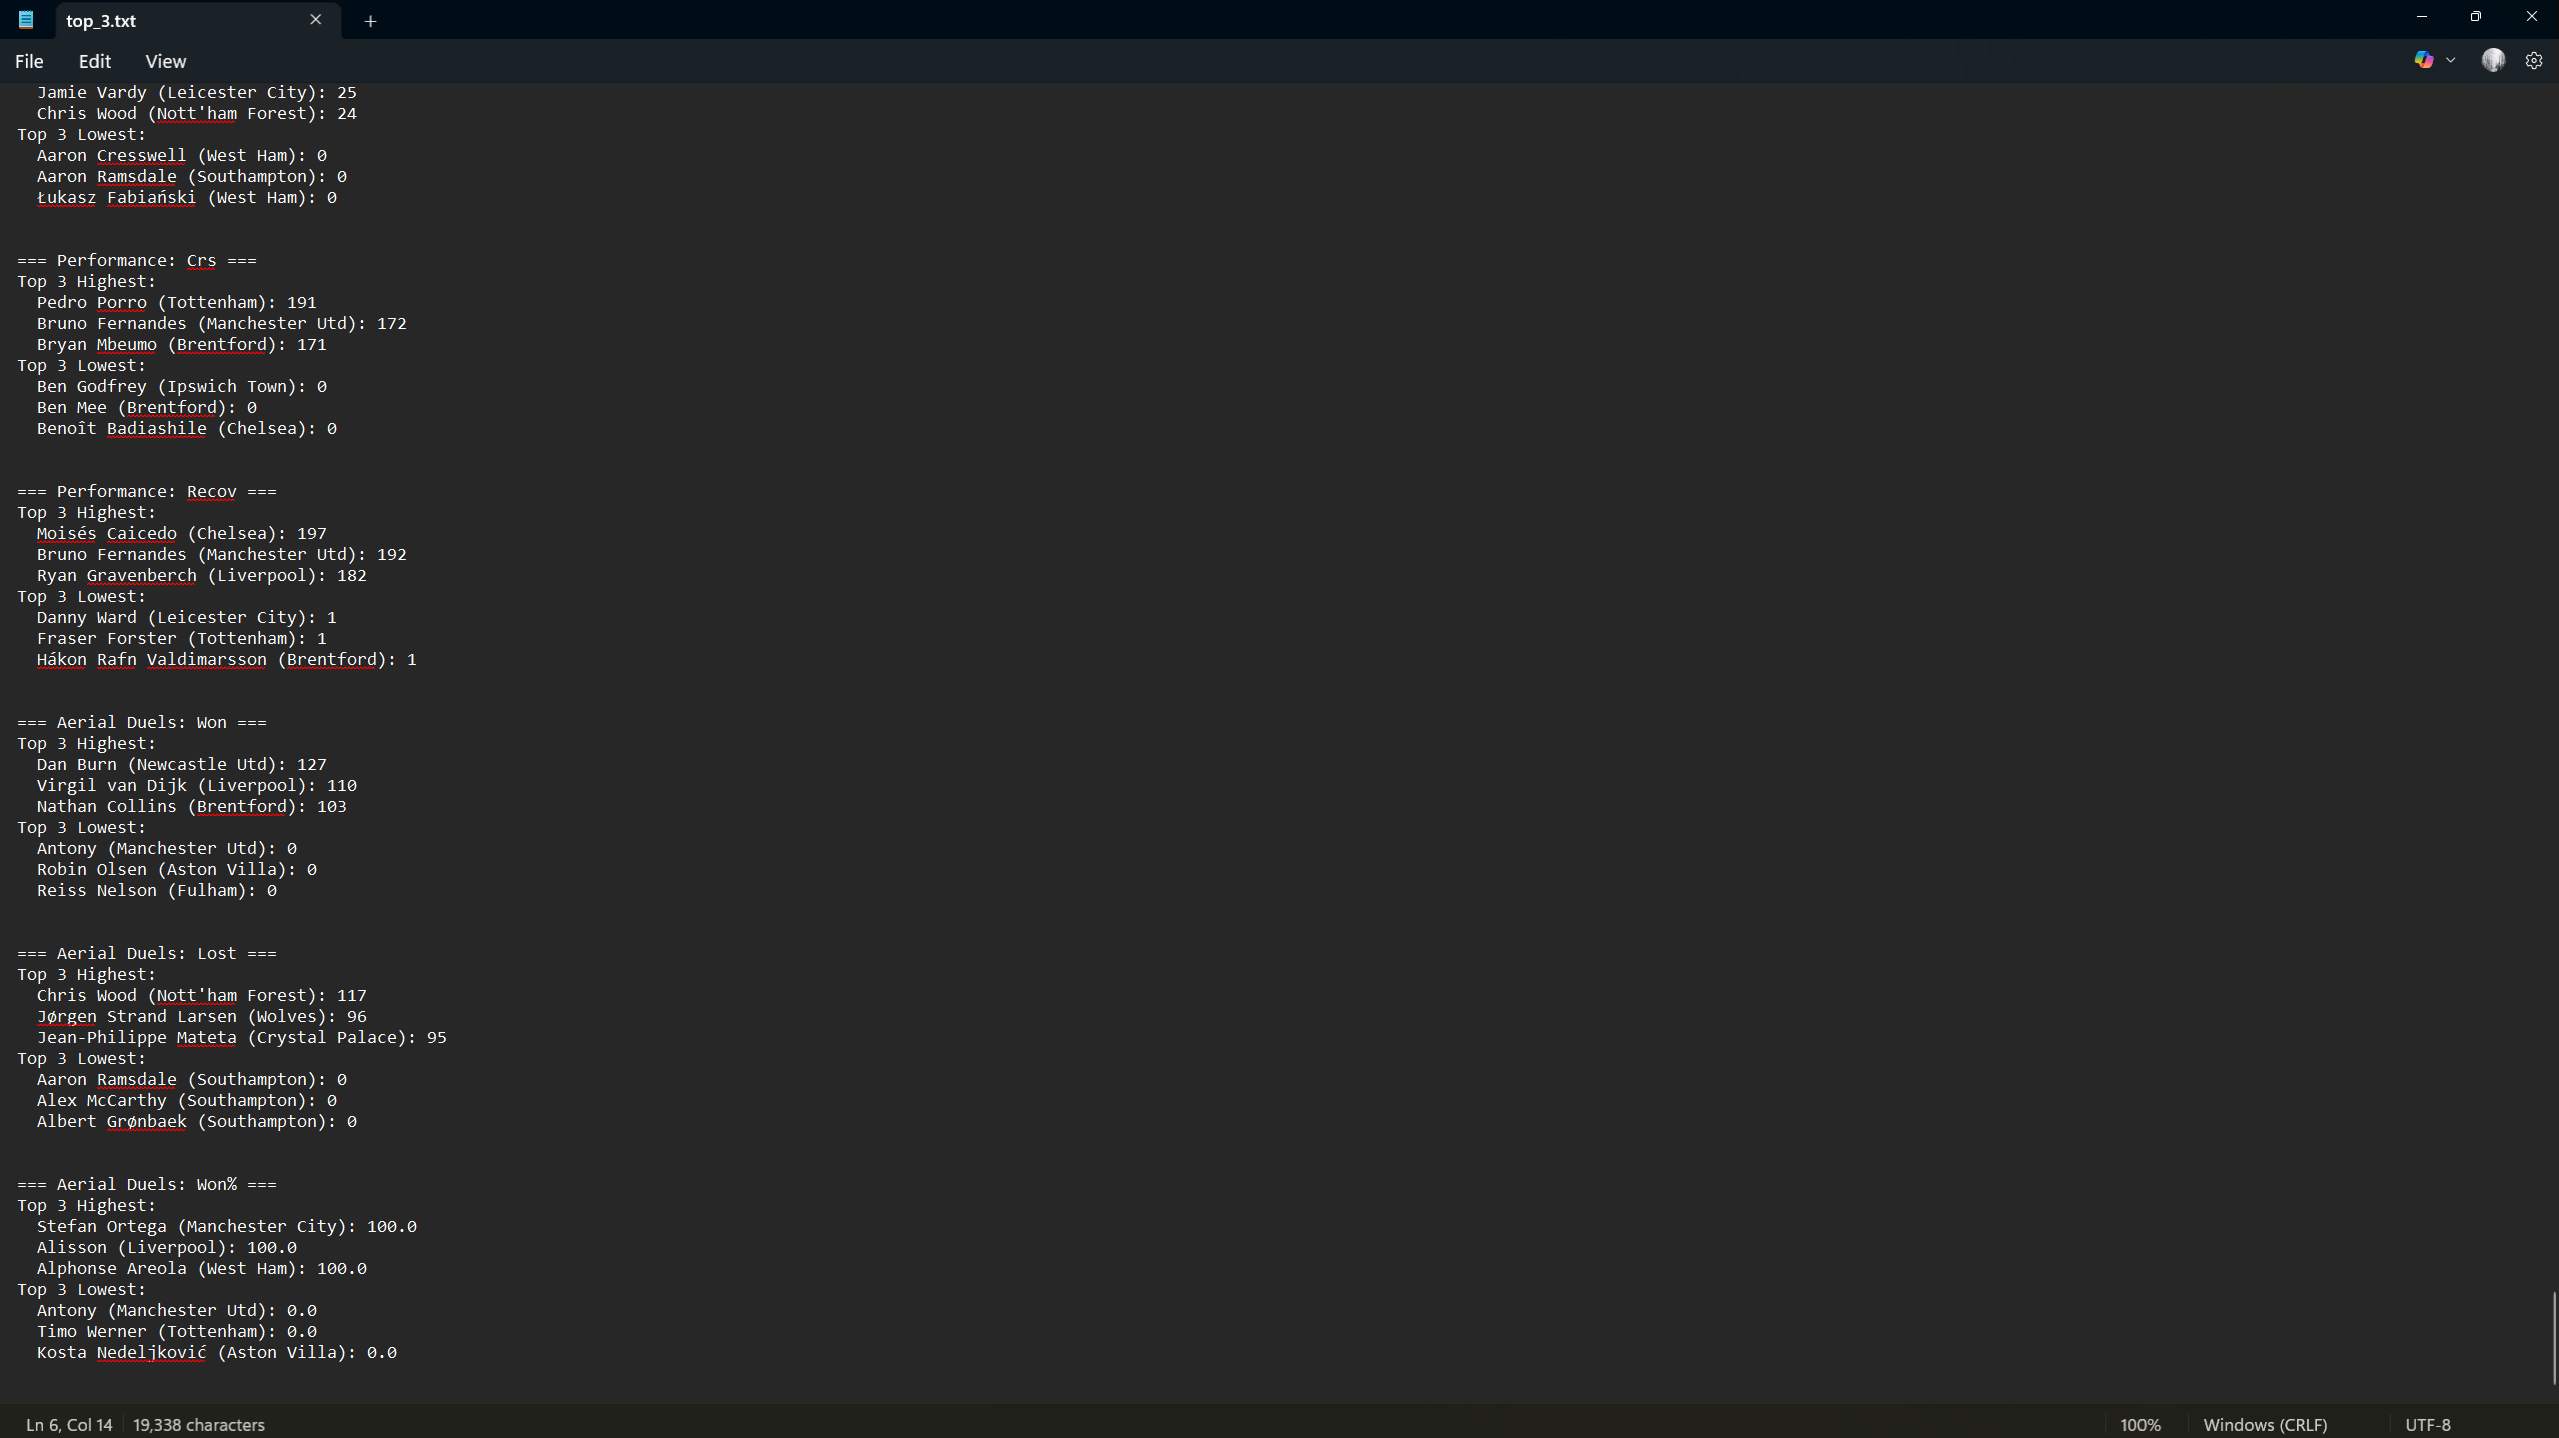
\includegraphics[width=220px]{top_3_1.png}
    \caption{File top\_3.txt} % Translated
    \label{fig:top3}
\end{figure}
\textbf{results2.csv} % Translated
The results2.csv file contains aggregate statistical data for teams in a league, with a total of 21 teams (or groups) and 220 feature columns related to match performance. Each row represents a team, including the team name and descriptive metrics for median, mean, and standard deviation across various aspects of play.
Recorded parameters include:
\begin{itemize}
	\item Playing time: matches played, starts, total minutes played;
	\item Technical performance metrics: such as aerial duels won/lost, aerial win percentage;
	\item Statistical format: each metric typically has 3 associated variables – Median, Mean, and Standard Deviation (Std), representing the data dispersion.
\end{itemize}
\begin{figure}[h]
    \centering
    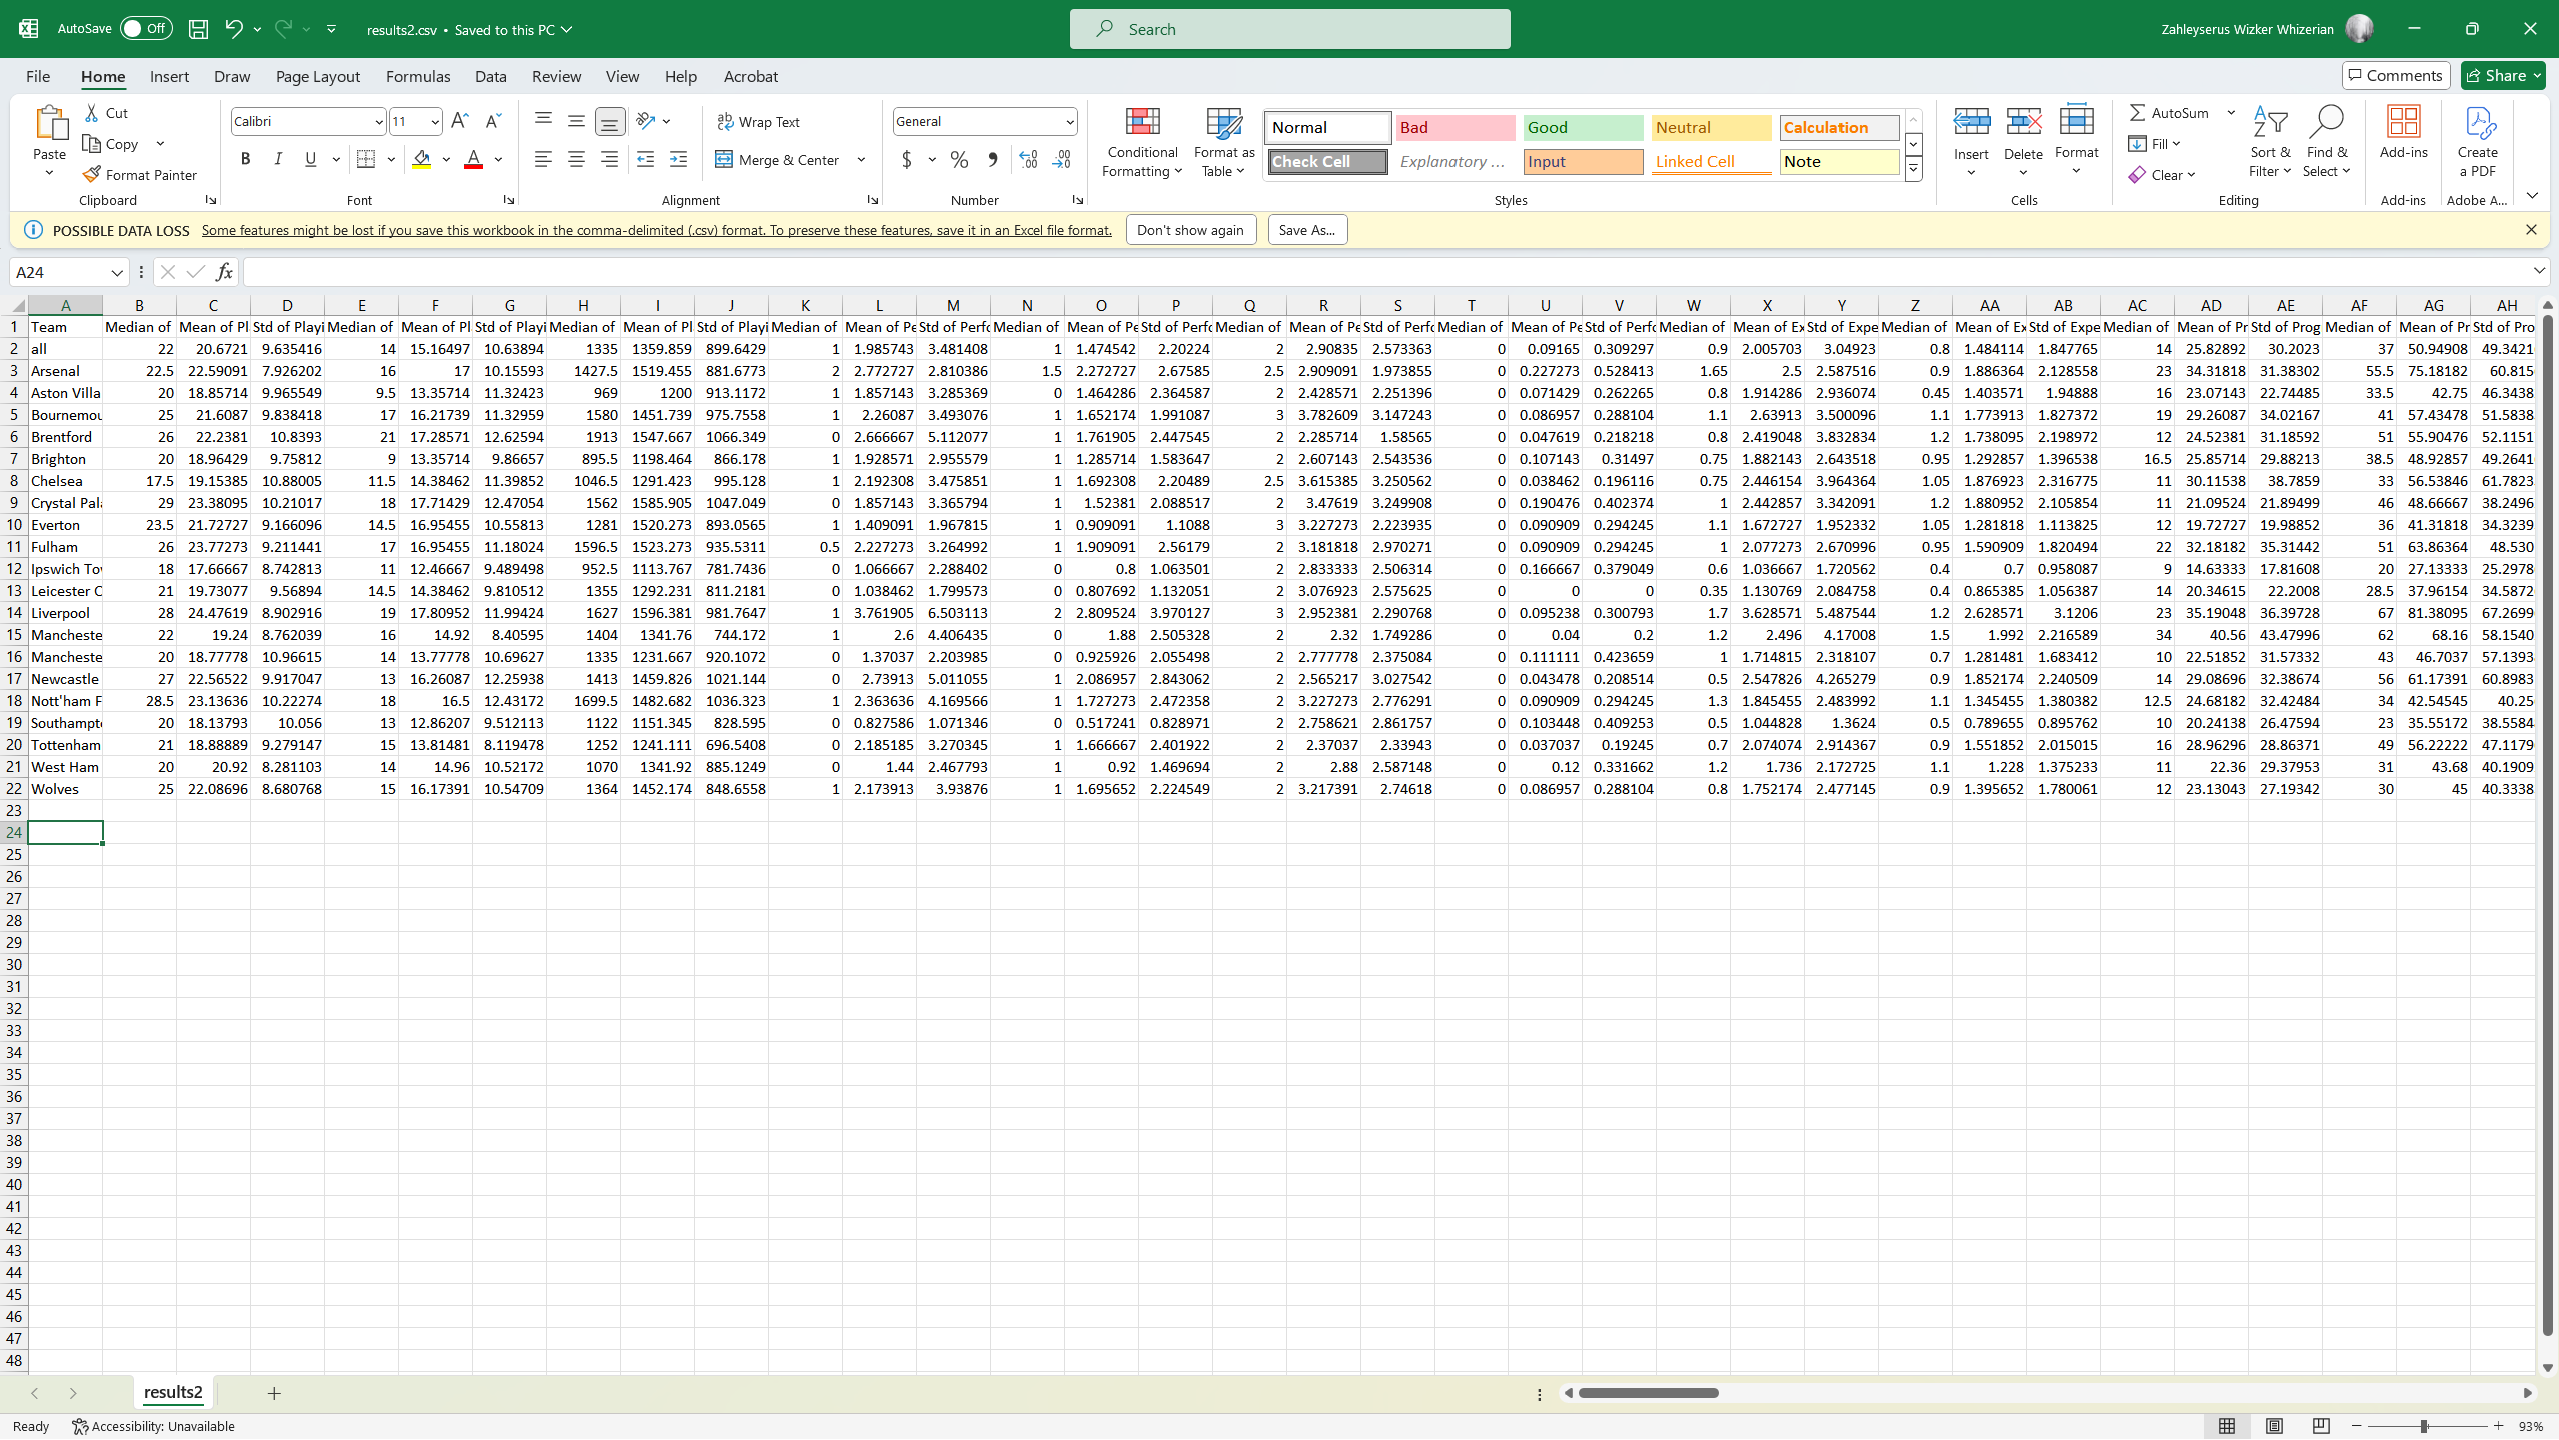
\includegraphics[width=220px]{results2.png}
    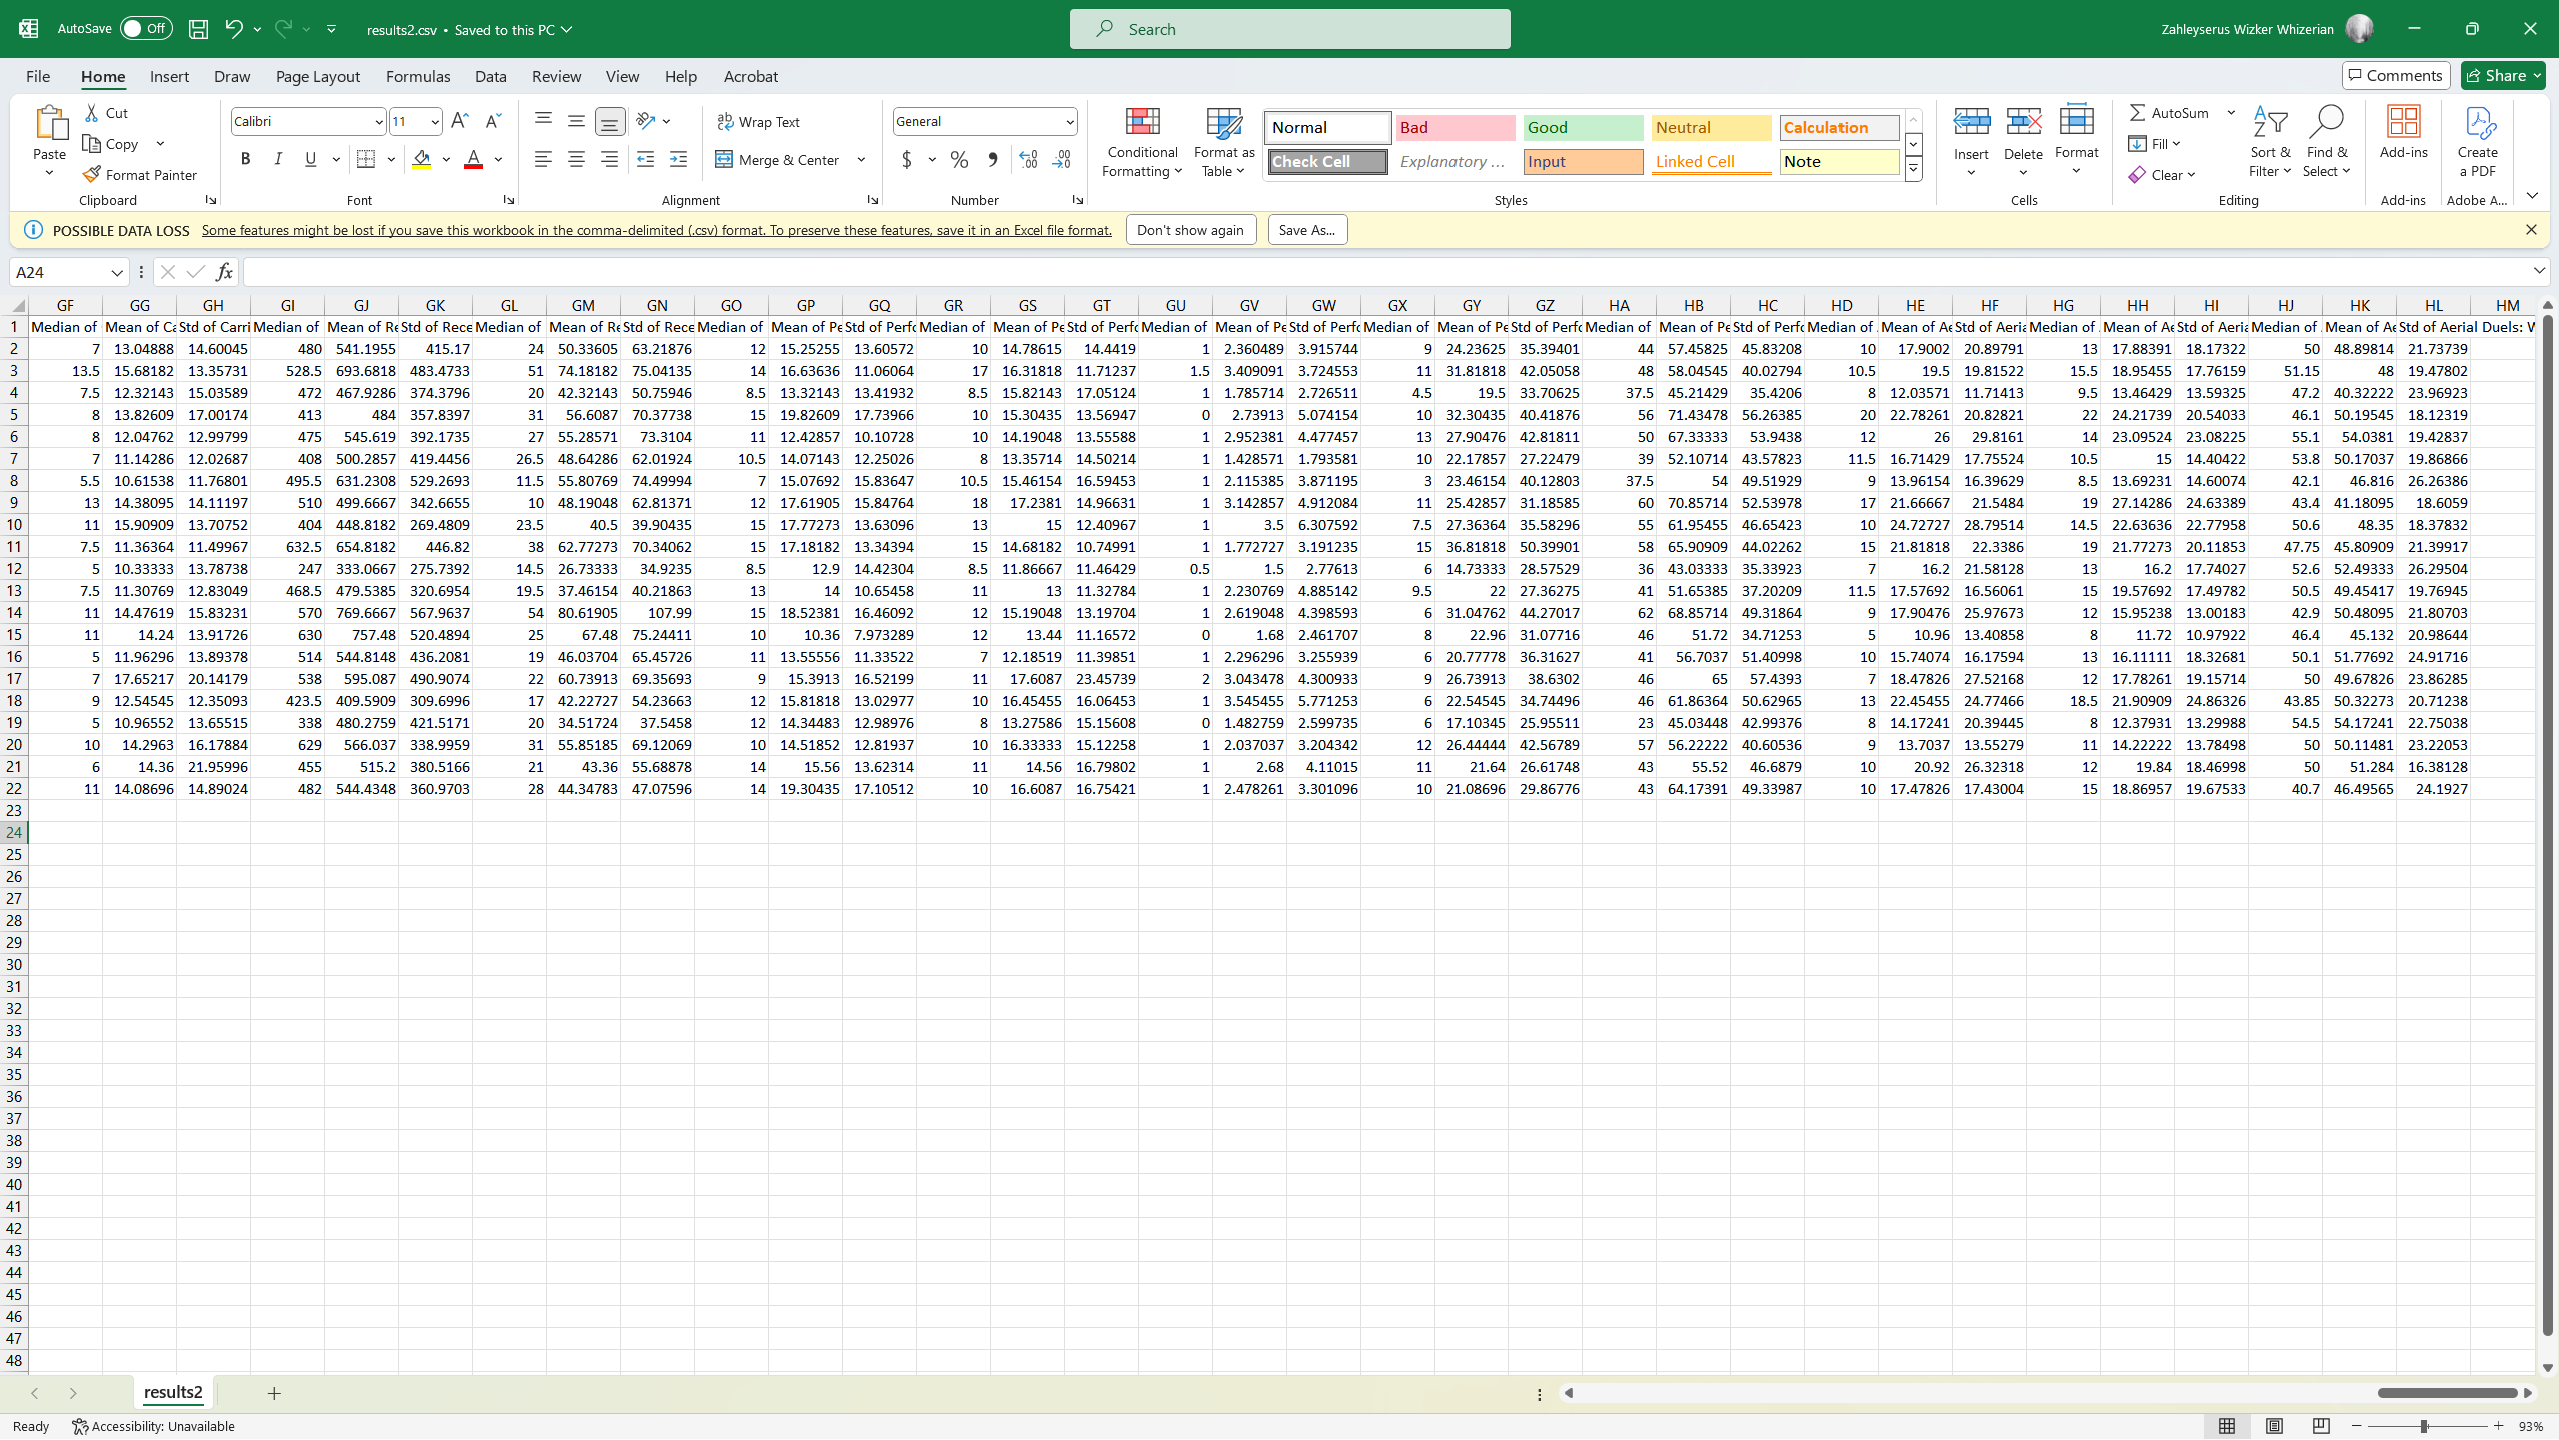
\includegraphics[width=220px]{results2_1.png}
    \caption{File results2.csv} % Translated
    \label{fig:res2}
\end{figure}
\textbf{Overall\_League\_Distribution\_of\_Player\_Indexes.png} % Translated
The image consists of 6 histogram plots arranged in a 2-column × 3-row grid, each plot having: % No direct citation, describes the image content based on structure.
\begin{itemize}
	\item A clear title at the top, describing the metric shown (e.g., Distribution of Performance: goals).
	\item The horizontal axis (X-axis) displays the specific metric name (like Performance: goals, Tackles: Tkl).
	\item The vertical axis (Y-axis) is labeled as Frequency, indicating the frequency of occurrence.
	\item Light blue histogram bars illustrate the data distribution.
\end{itemize}
A dark blue KDE curve is smoothly plotted over the data distribution to visualize the probability density. The entire image has a neat layout, uniform presentation style, and axis formatting, making it easy to compare across plots.
\begin{figure}[h]
    \centering
    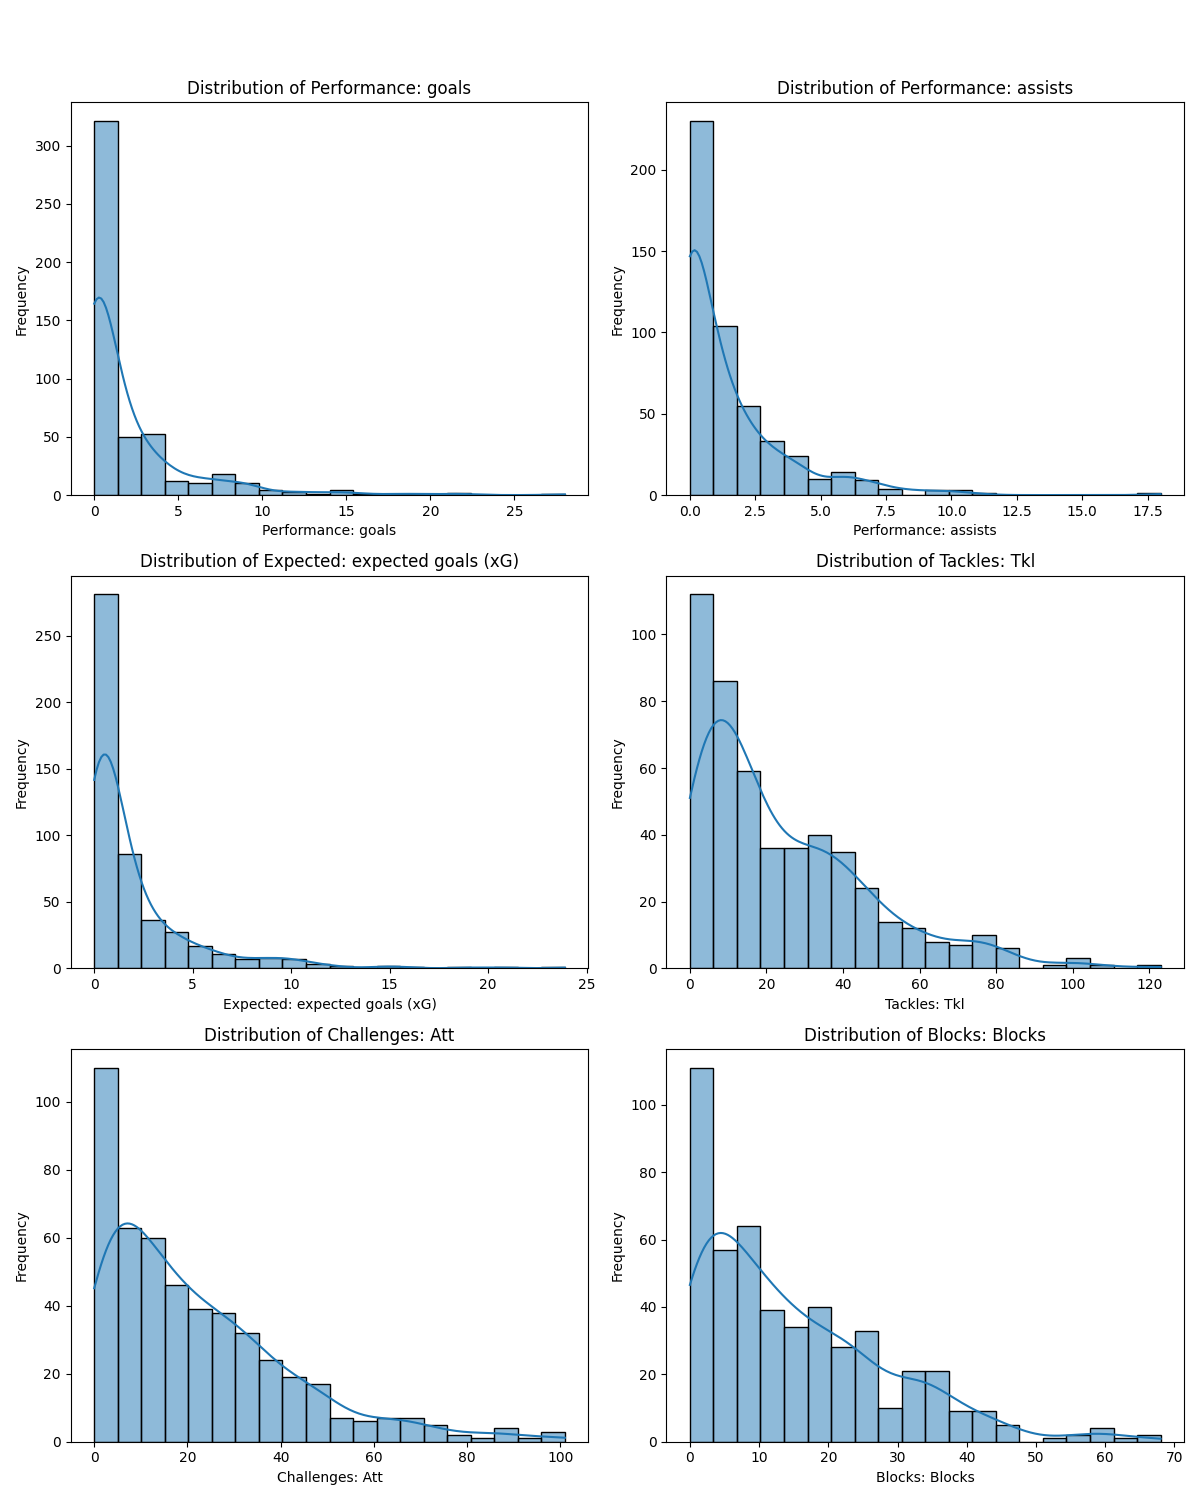
\includegraphics[width=400px]{Overall_League_Distribution_of_Player_Indexes.png}
    \caption{File Overall\_League\_Distribution\_of\_Player\_Indexes.png} % Translated
    \label{fig:p1}
\end{figure}
\begin{figure}[h]
    \centering
    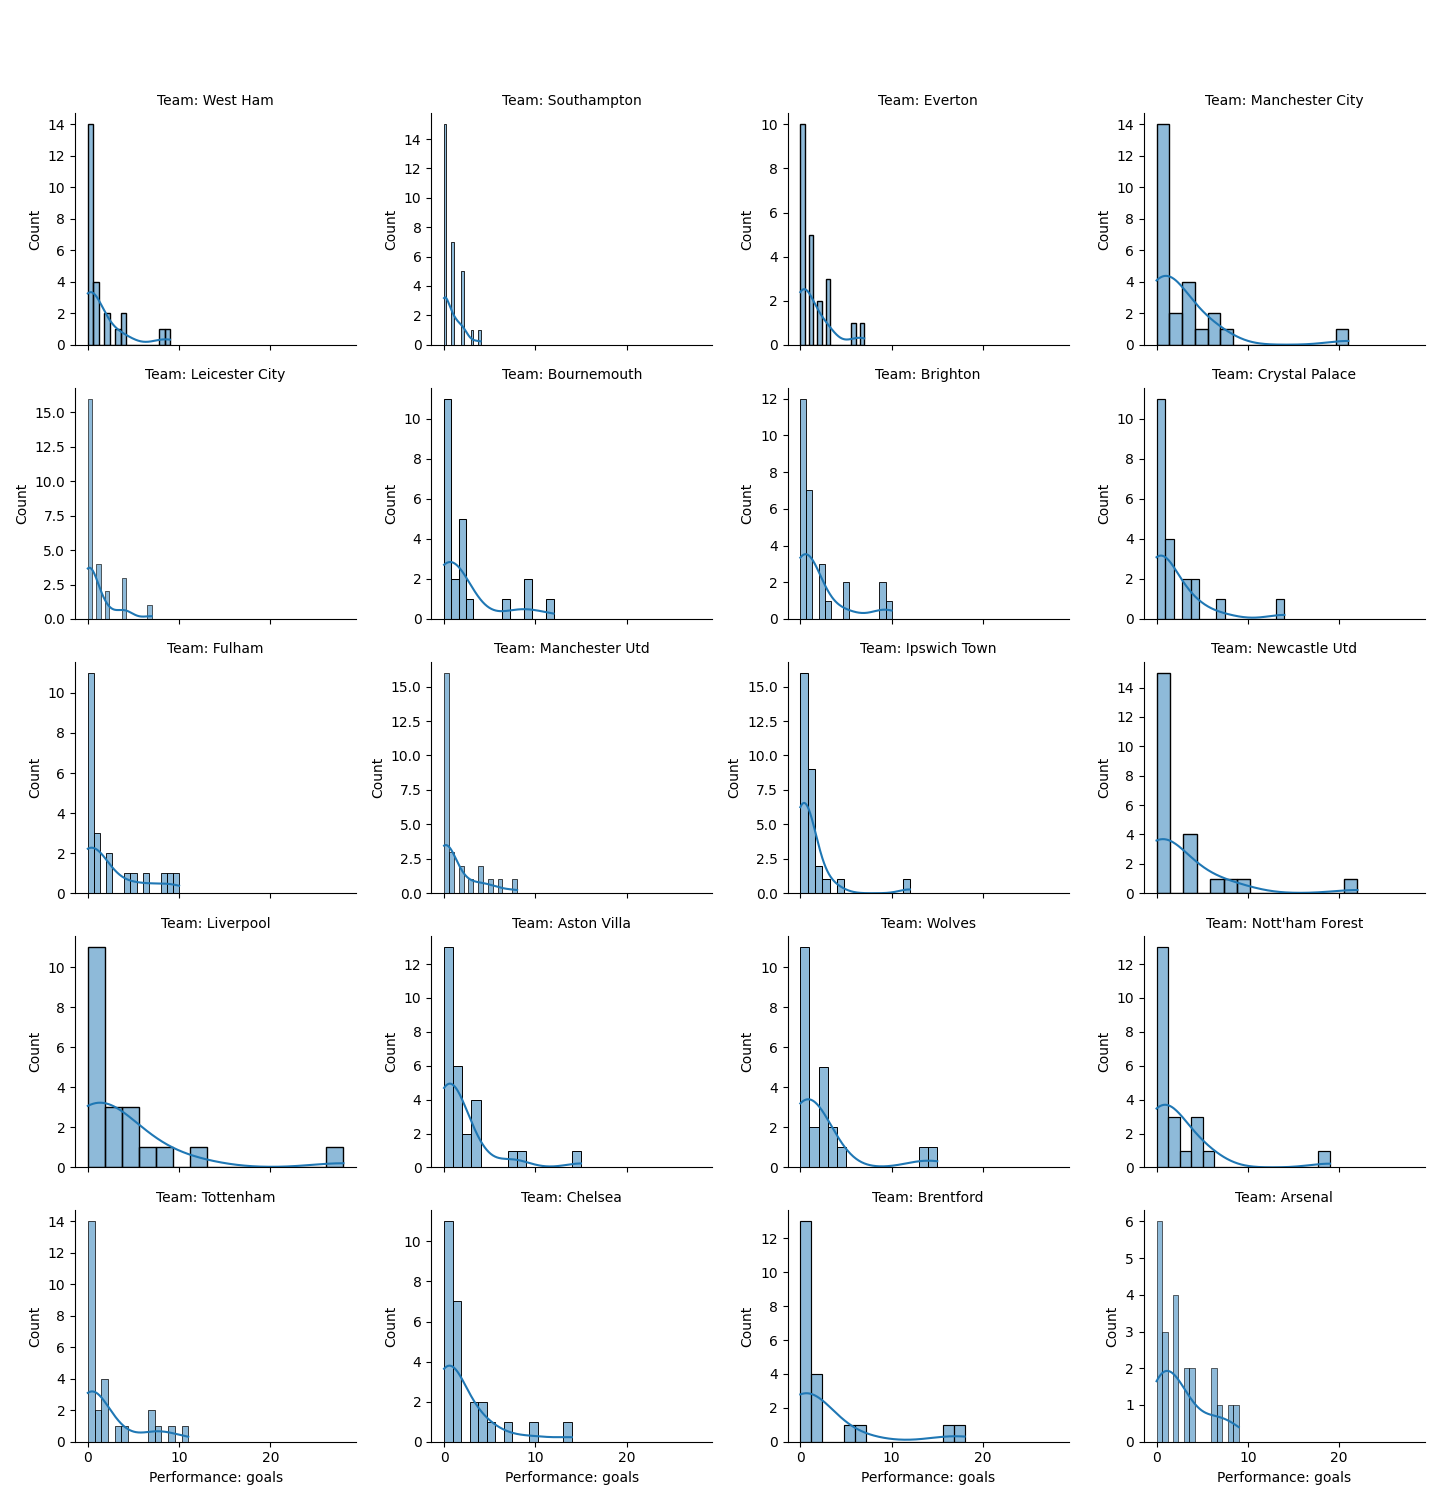
\includegraphics[width=300px]{Distribution_of_Performance_goals_by_Team.png}
    \caption{File Distribution\_of\_Performance\_goals\_by\_Team.png} % Translated
    \label{fig:p2}
\end{figure}
\begin{figure}[h]
    \centering
    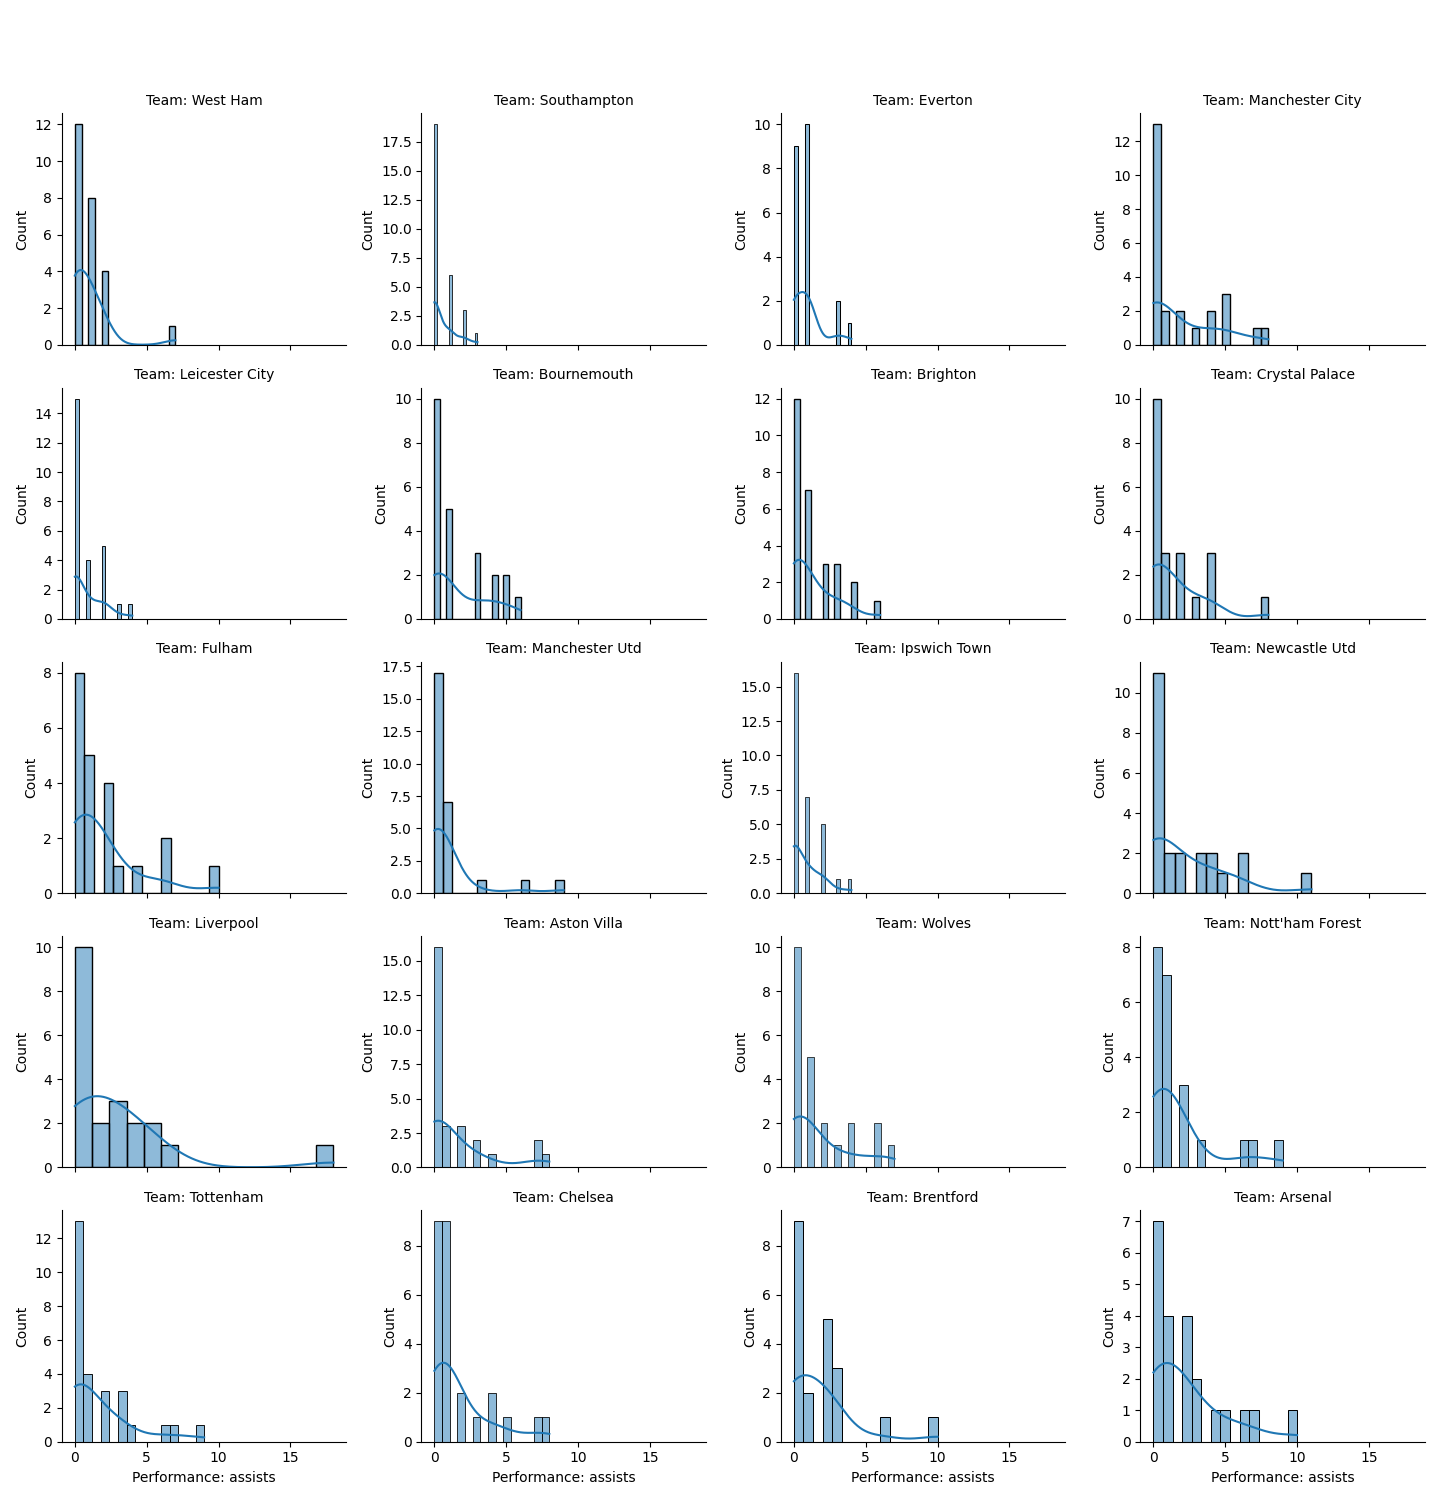
\includegraphics[width=300px]{Distribution_of_Performance_assists_by_Team.png}
    \caption{File Distribution\_of\_Performance\_assists\_by\_Team.png} % Translated
    \label{fig:p3}
\end{figure}
\begin{figure}[h]
    \centering
    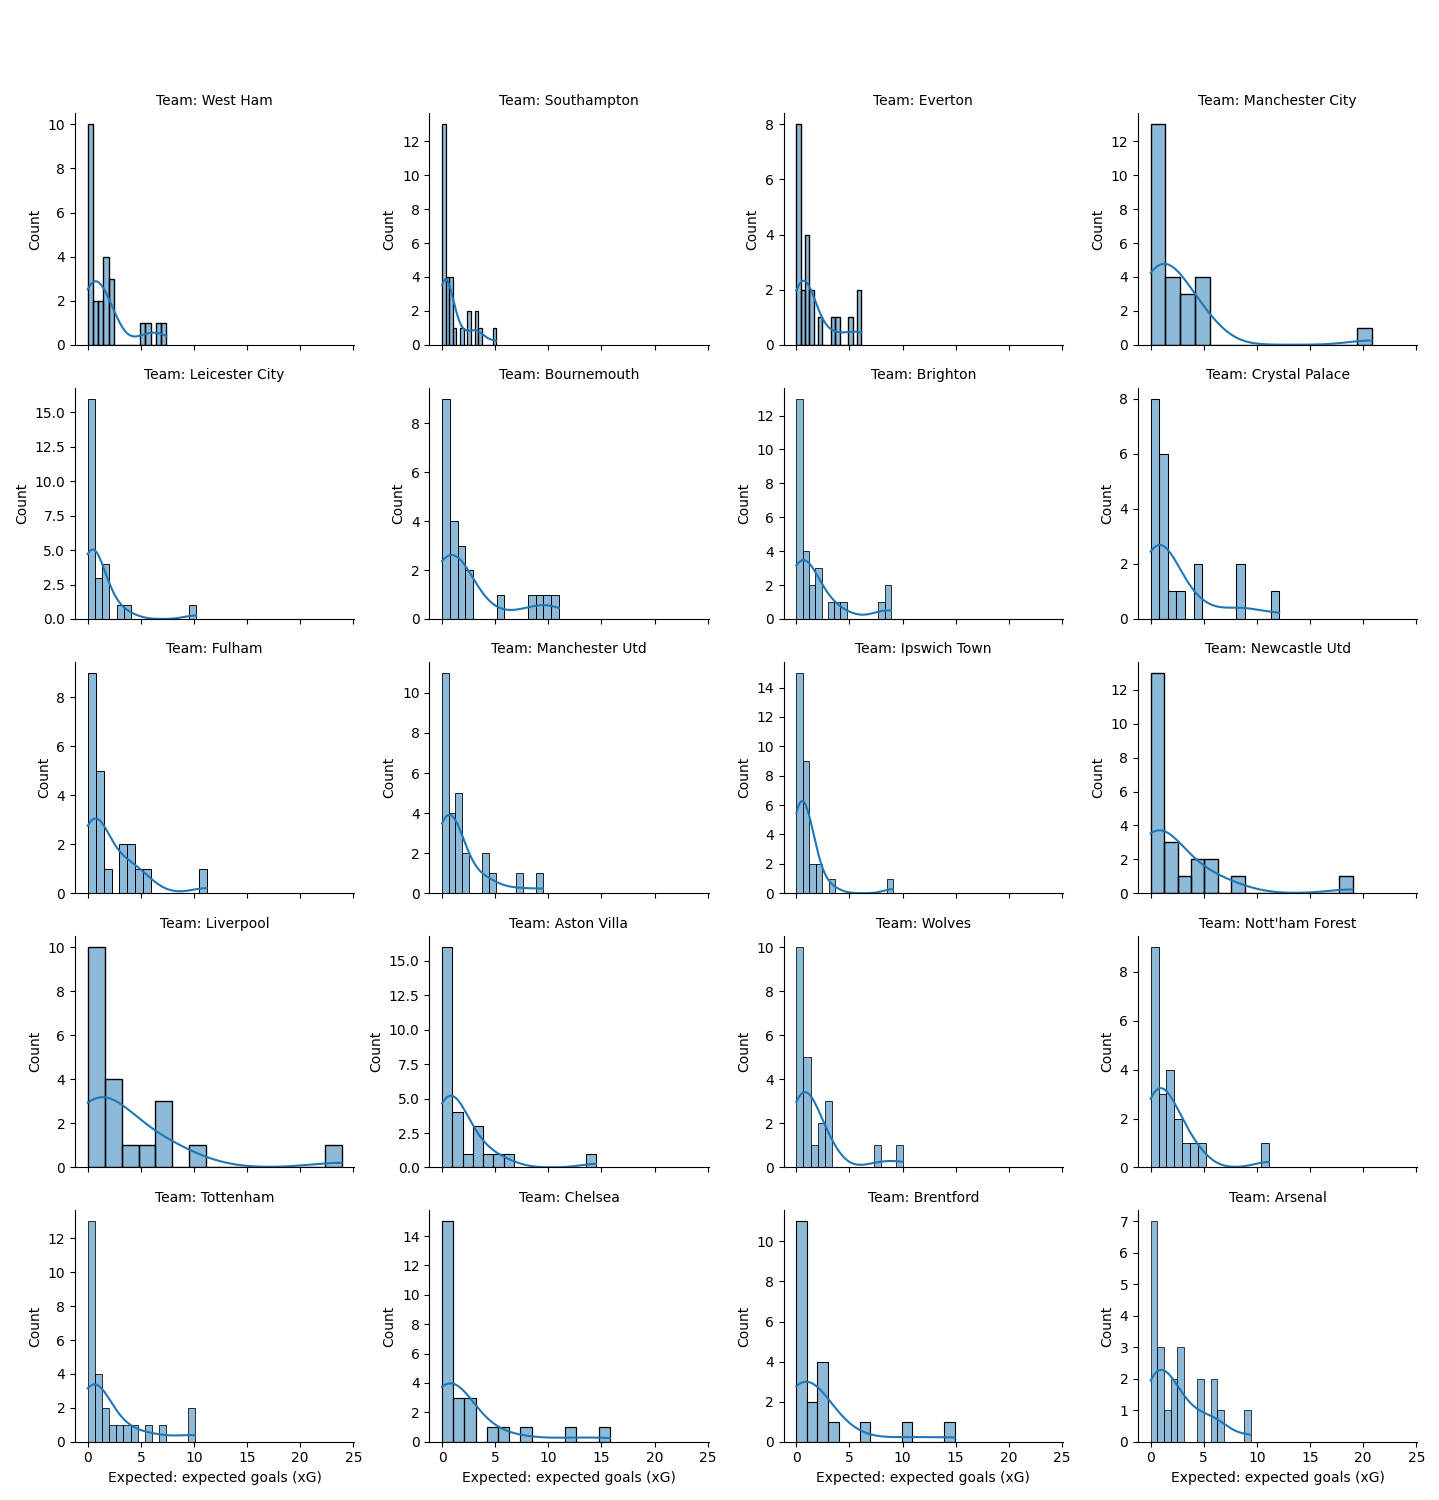
\includegraphics[width=300px]{Distribution_of_Expected_expected_goals_(xG)_by_Team.png}
    \caption{File Distribution\_of\_Expected\_expected\_goals\_(xG)\_by\_Team.png} % Translated
    \label{fig:p4}
\end{figure}
\begin{figure}[h]
    \centering
    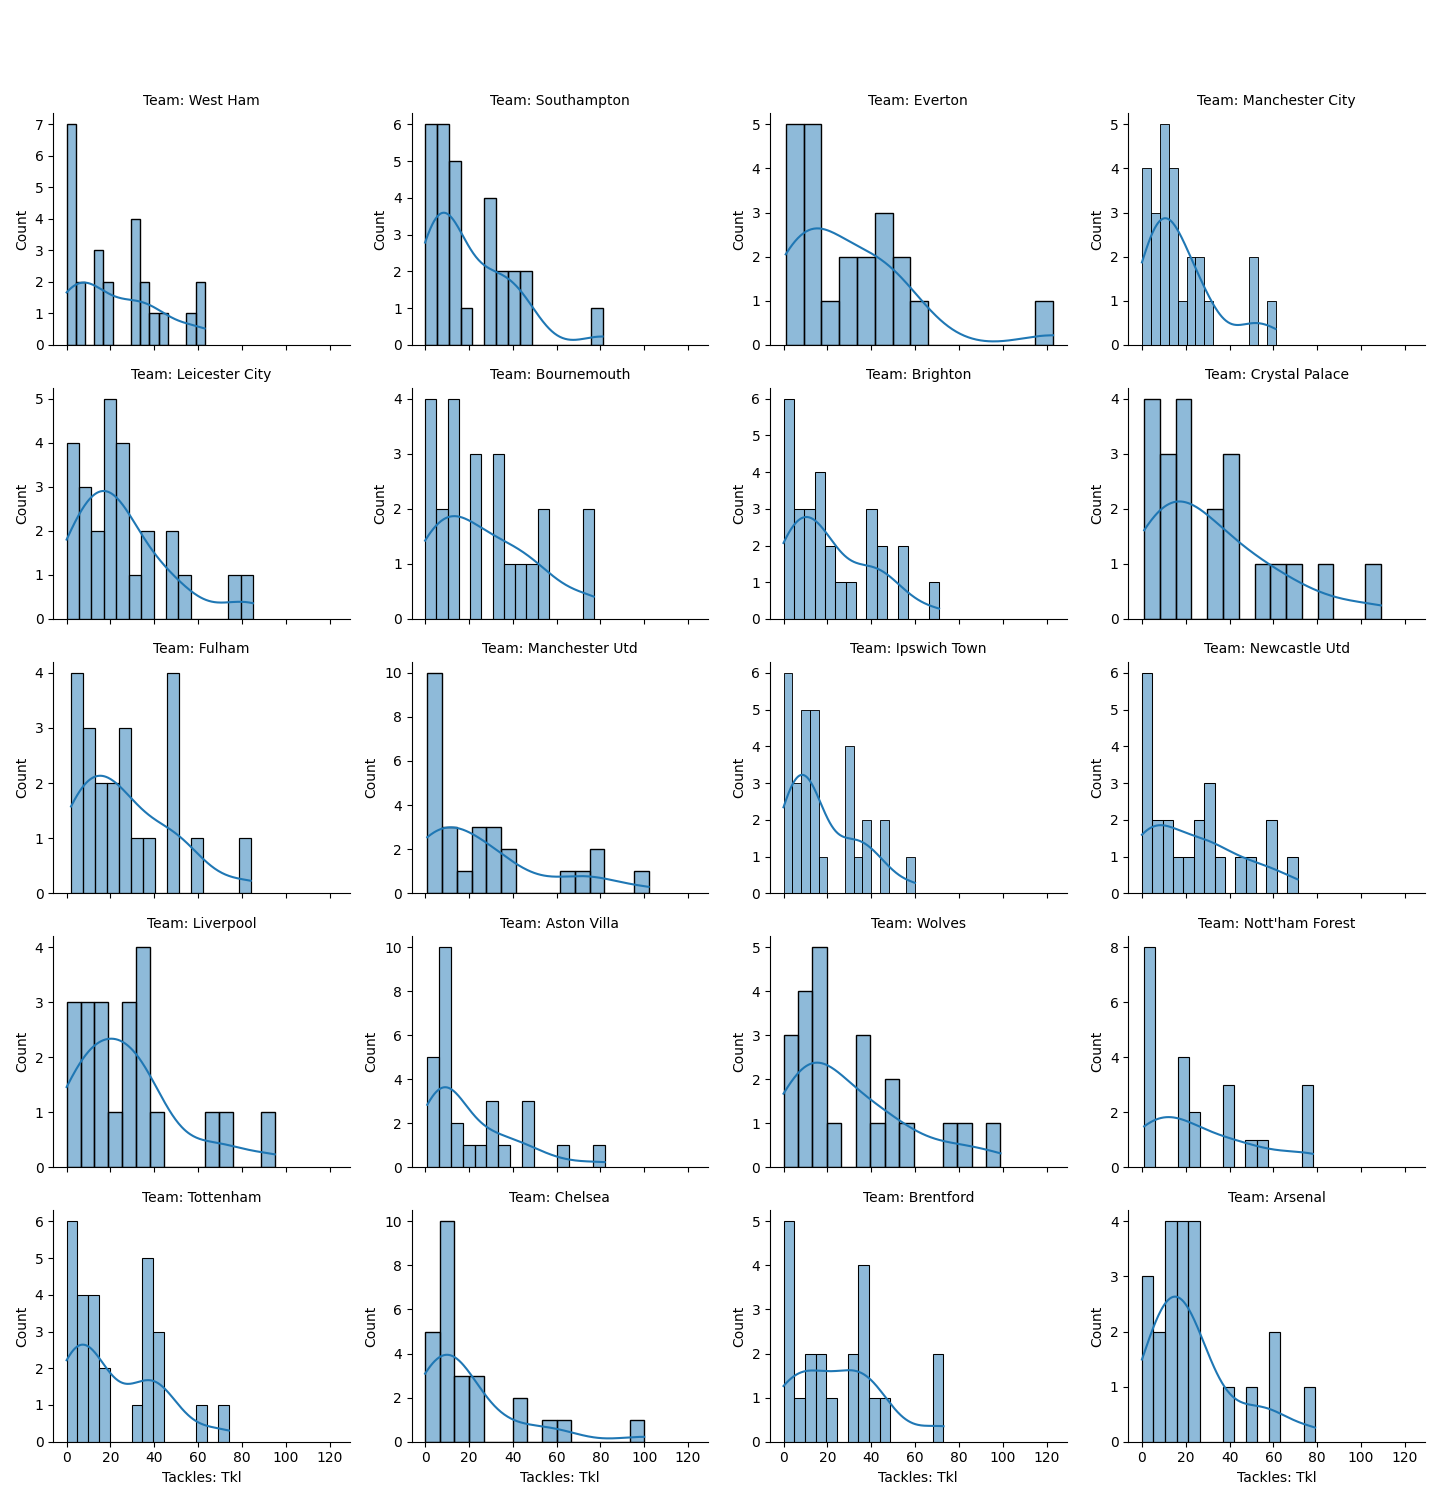
\includegraphics[width=300px]{Distribution_of_Tackles_Tkl_by_Team.png}
    \caption{File Distribution\_of\_Tackles\_Tkl\_by\_Team.png} % Translated
    \label{fig:p5}
\end{figure}
\begin{figure}[h]
    \centering
    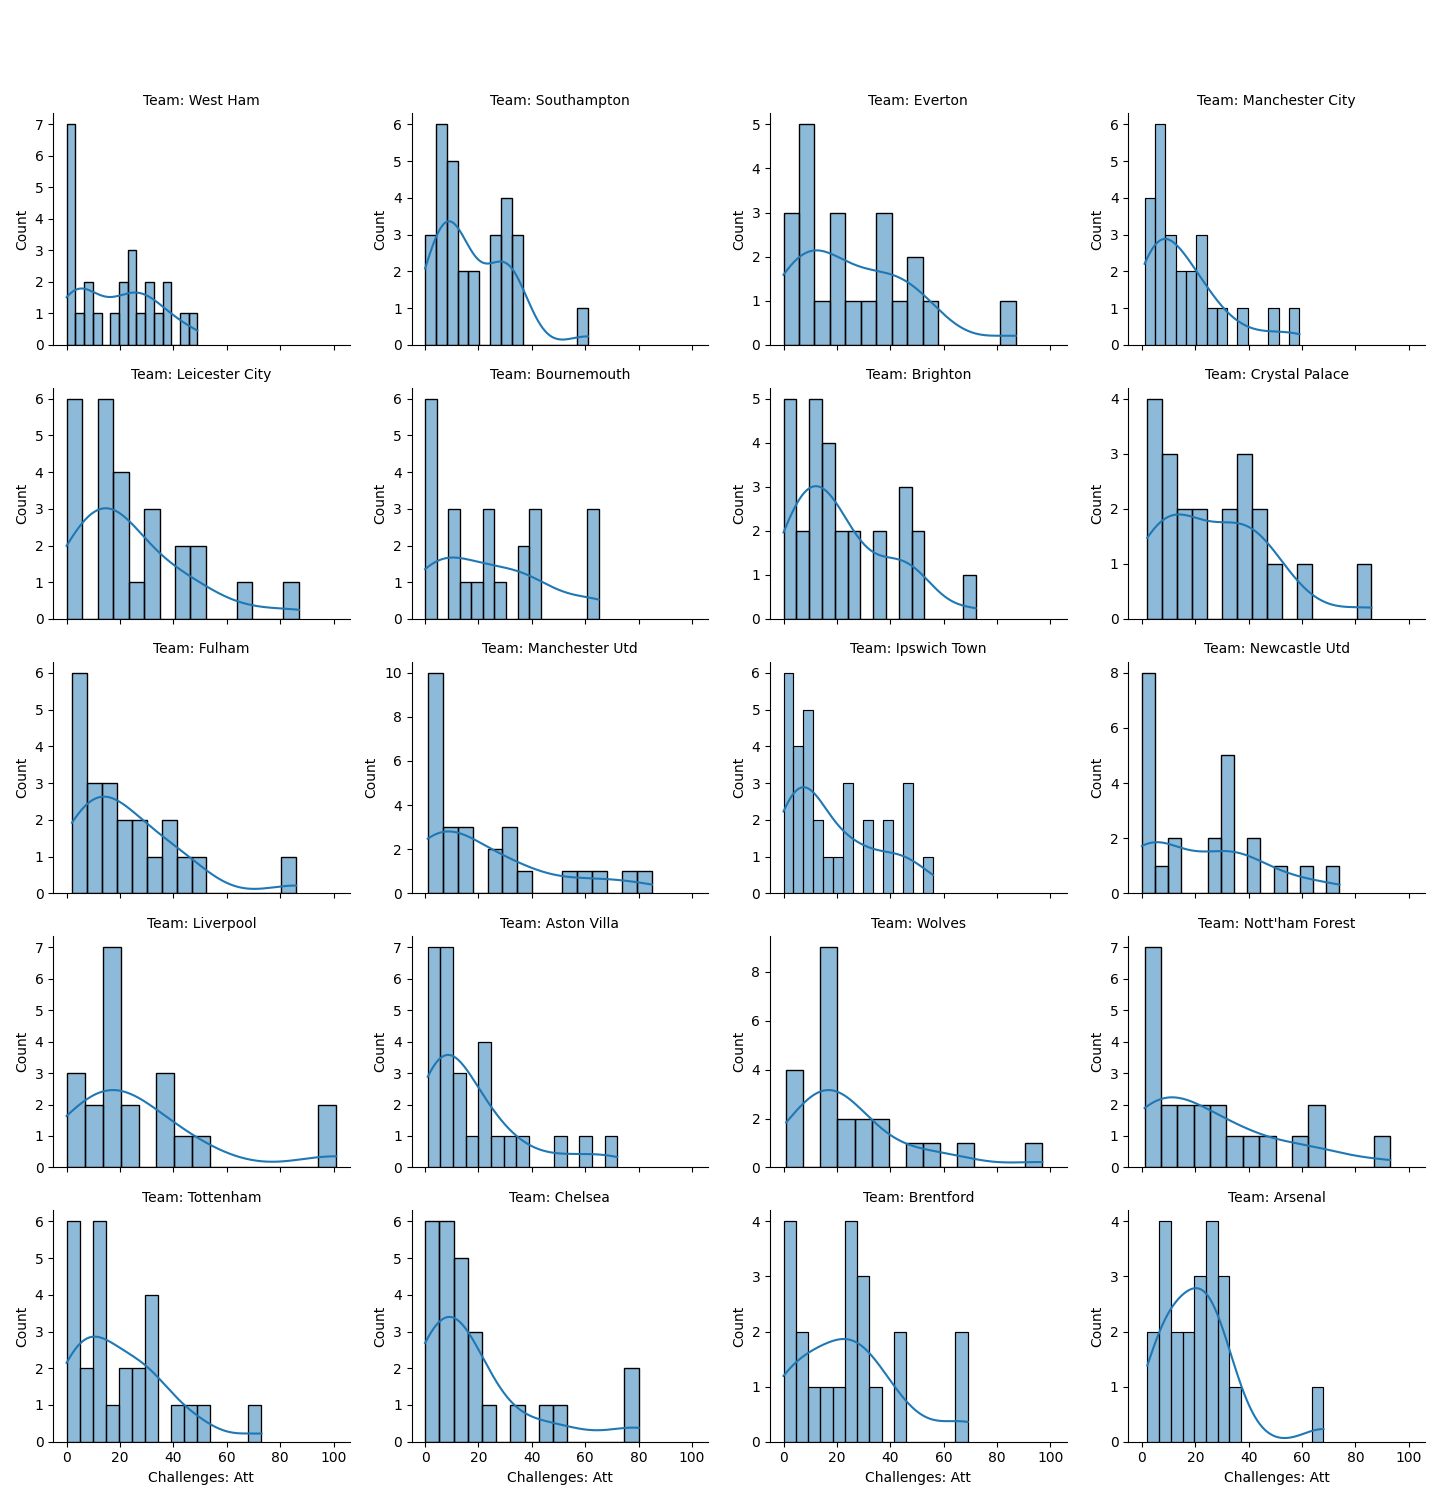
\includegraphics[width=300px]{Distribution_of_Challenges_Att_by_Team.png}
    \caption{File Distribution\_of\_Challenges\_Att\_by\_Team.png} % Translated
  \label{fig:p6}
\end{figure}
\begin{figure}[h]
    \centering
    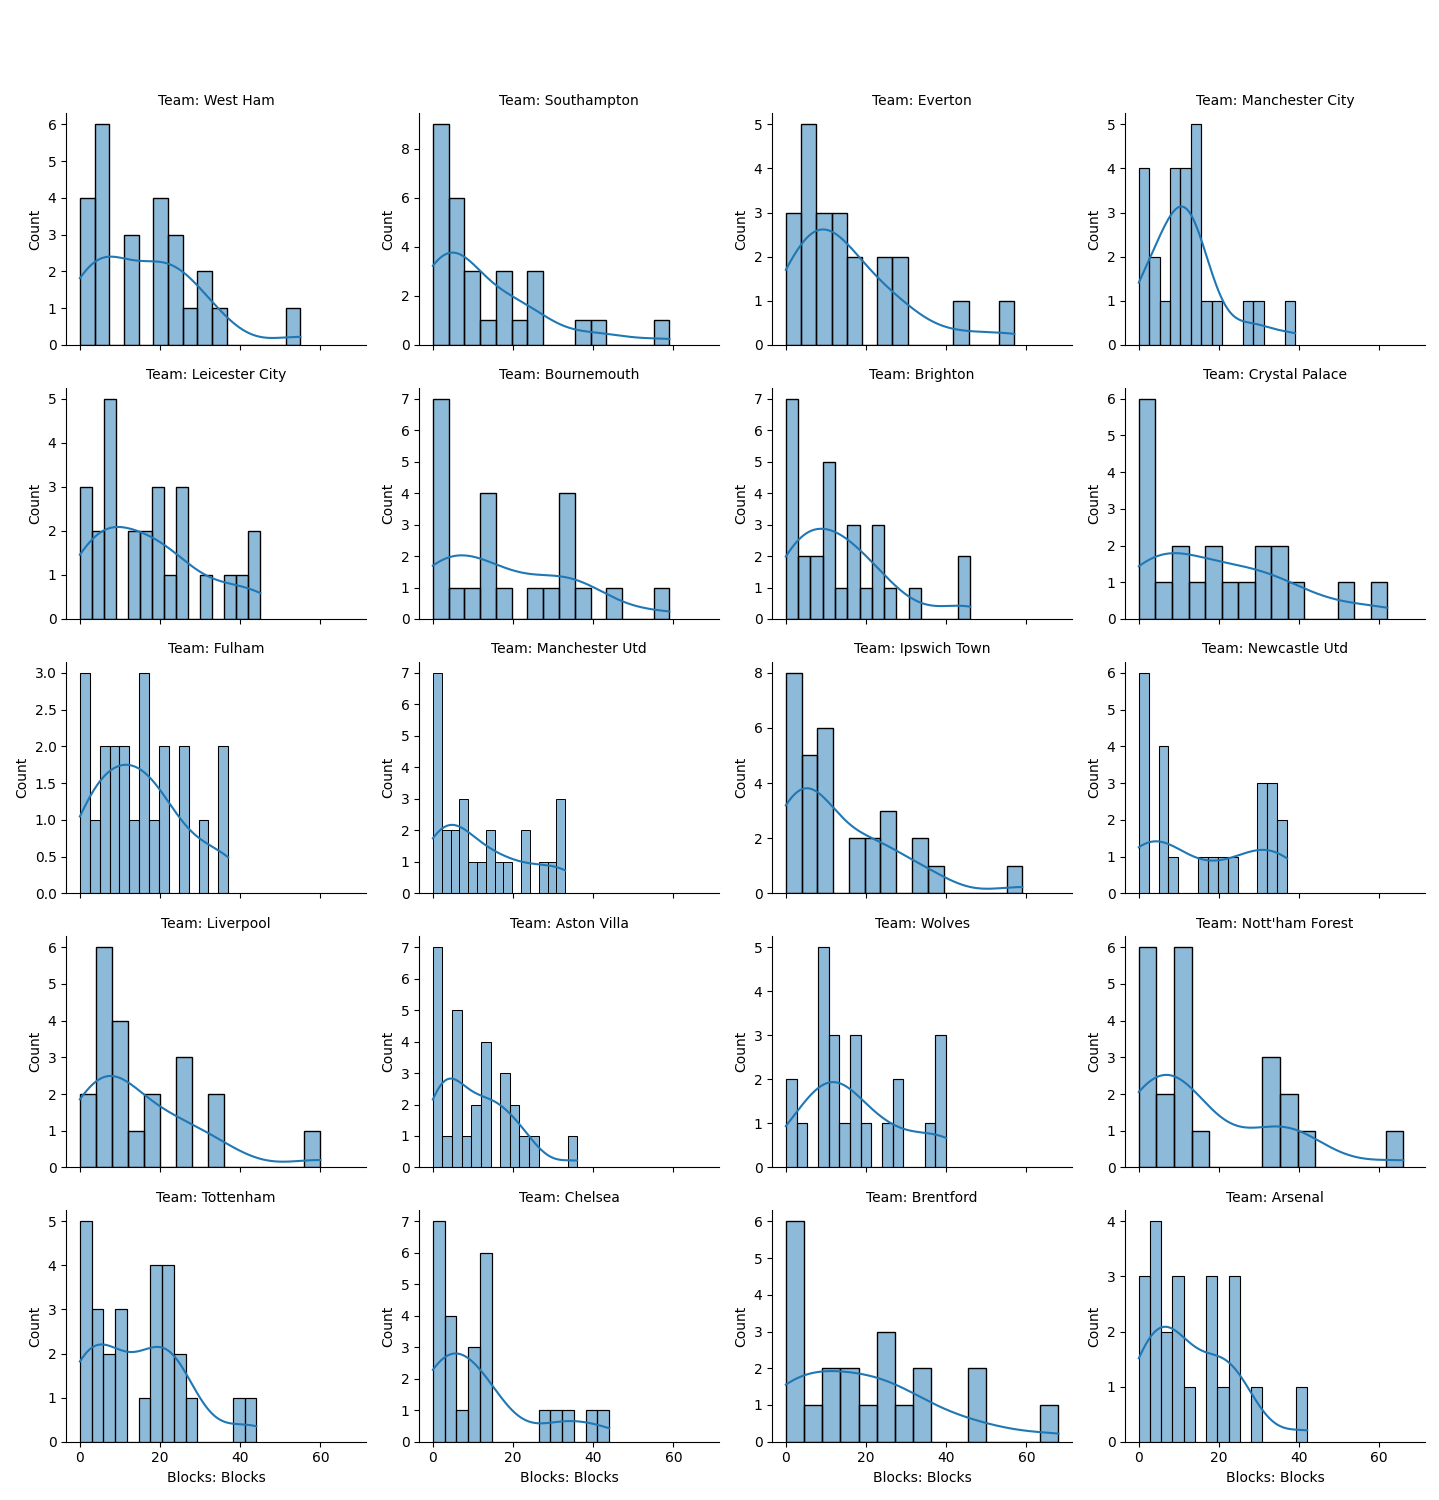
\includegraphics[width=300px]{Distribution_of_Blocks_Blocks_by_Team.png}
    \caption{File Distribution\_of\_Blocks\_Blocks\_by\_Team.png} % Translated
    \label{fig:p7}
\end{figure}
\clearpage
\textbf{Distribution\_of\_Performance\_goals\_by\_Team.png:} % Translated
The image displays a grid matrix of histogram charts consisting of 24 subplots (4 rows × 6 columns), each representing a different team in the league. % Describes structure
Regarding the format: % Describes format
\begin{itemize}
	\item The title of each chart is at the top, clearly stating the team name (e.g., Team: Manchester City, Team: Arsenal).
	\item The horizontal axis (X-axis) is consistently labeled as Performance: goals, representing the number of goals.
	\item The vertical axis (Y-axis) is marked as Count, indicating the number of players achieving the corresponding goal level.
	\item Light blue histogram bars, accompanied by a dark blue KDE curve, represent the probability density distribution of goals for players within each team.
\end{itemize}
The entire layout is arranged evenly, with uniform proportions and style, facilitating easy comparison of goal distribution among teams. This visualization style is commonly used in sports statistics reports or multi-group quantitative data analysis.

\textbf{Distribution\_of\_Performance\_assists\_by\_Team.png:} % Translated
This image is a visual layout in a grid format comprising 24 small histogram charts, each representing a different team in the league. In terms of appearance, the image has the following characteristics:
\begin{itemize}
	\item A grid structure of 6 columns × 4 rows, helping to organize the charts evenly and make them easy to follow.
	\item Each subplot has a title at the top clearly indicating the team name, e.g., Team: Arsenal, Team: Manchester Utd, etc.
	\item The horizontal axis on all charts is labeled Performance: goals, showing the number of goals scored by players.
	\item The vertical axis is labeled Count, representing the number of players corresponding to each goal level.
	\item Within each chart, light blue histogram bars represent frequency, accompanied by a dark blue KDE curve showing the probability density distribution.
	\item The style, axis proportions, and chart layout are kept consistent across teams, creating a clear visual whole, making it easy to compare goal distributions between teams.
\end{itemize}
Overall, the image is presented in a scientific style and standard data visualization manner, suitable for academic reports or quantitative statistical analysis in the field of sports.

\textbf{Distribution\_of\_Expected\_expected\_goals\_(xG)\_by\_Team.png:} % Translated
This image is a visual layout in a grid format comprising 24 small histogram charts, each representing a different team in the league. In terms of appearance, the image has the following characteristics:
\begin{itemize}
	\item A grid structure of 6 columns × 4 rows, helping to organize the charts evenly and make them easy to follow.
	\item Each subplot has a title at the top clearly indicating the team name, e.g., Team: Arsenal, Team: Manchester Utd, etc.
	\item The horizontal axis on all charts is labeled Performance: expected\_goals (xG), showing the expected goals created by players.
	\item The vertical axis is labeled Count, representing the number of players corresponding to each xG level.
	\item Within each chart, light blue histogram bars represent frequency, accompanied by a dark blue KDE curve showing the probability density distribution.
	\item The style, axis proportions, and chart layout are kept consistent across teams, creating a clear visual whole, making it easy to compare xG distributions between teams.
\end{itemize}
Overall, the image is presented in a scientific style and standard data visualization manner, suitable for academic reports or quantitative statistical analysis in the field of sports.

\textbf{Distribution\_of\_Tackles\_Tkl\_by\_Team.png:} % Translated
The image is a visual layout consisting of 24 small charts arranged in a 6x4 grid.
\begin{itemize}
	\item The title of each subplot clearly identifies the team name.
	\item The horizontal axis is Performance: tackles\_tkl, reflecting the number of tackles made by players.
	\item The vertical axis is Count, indicating the number of players achieving the corresponding tackle level.
	\item Light blue histograms and dark blue KDE curves continue to be the main form of representation.
	\item Consistency in proportions, colors, layout, and formatting is maintained.
\end{itemize}
The chart provides strong visualization for active defensive statistics (tackles) of the teams.

\textbf{Distribution\_of\_Challenges\_Att\_by\_Team.png:} % Translated
This visual image also comprises 24 small charts arranged in a 6x4 grid, each representing a team.
\begin{itemize}
	\item The title of each subplot follows the format Team: [Team Name].
	\item The horizontal axis reads Performance: challenges\_att, indicating the number of challenges attempted.
	\item The vertical axis is Count, reflecting the number of players corresponding to each challenge level.
	\item Light blue histogram bars combined with dark blue KDE lines remain the primary method of presentation.
	\item Proportions and framing maintain absolute consistency across teams, facilitating easy comparison.
\end{itemize}
The image provides good visualization for statistics related to the challenge strength of each team.

\textbf{Distribution\_of\_Blocks\_Blocks\_by\_Team.png:} % Translated
This image is a visual layout in a grid format comprising 24 small histogram charts, each representing a different team. In terms of appearance:
\begin{itemize}
	\item The 6 column × 4 row grid structure is maintained.
	\item The title above each subplot shows the team name, e.g., Team: Chelsea, Team: Leeds, etc.
	\item The horizontal axis is labeled Performance: blocks, representing the number of blocks performed by players.
	\item The vertical axis is Count, indicating the number of players corresponding to each block level.
	\item Light blue histograms represent frequency, combined with dark blue KDE lines to show the distribution trend.
	\item Layout, proportions, and style are synchronized, ensuring easy comparison between teams.
\end{itemize}
Overall, the image maintains a professional style with high consistency, effectively supporting the analysis of defensive performance among teams.

\textbf{best\_team\_summary.txt:} % Translated
\begin{figure}[h]
    \centering
    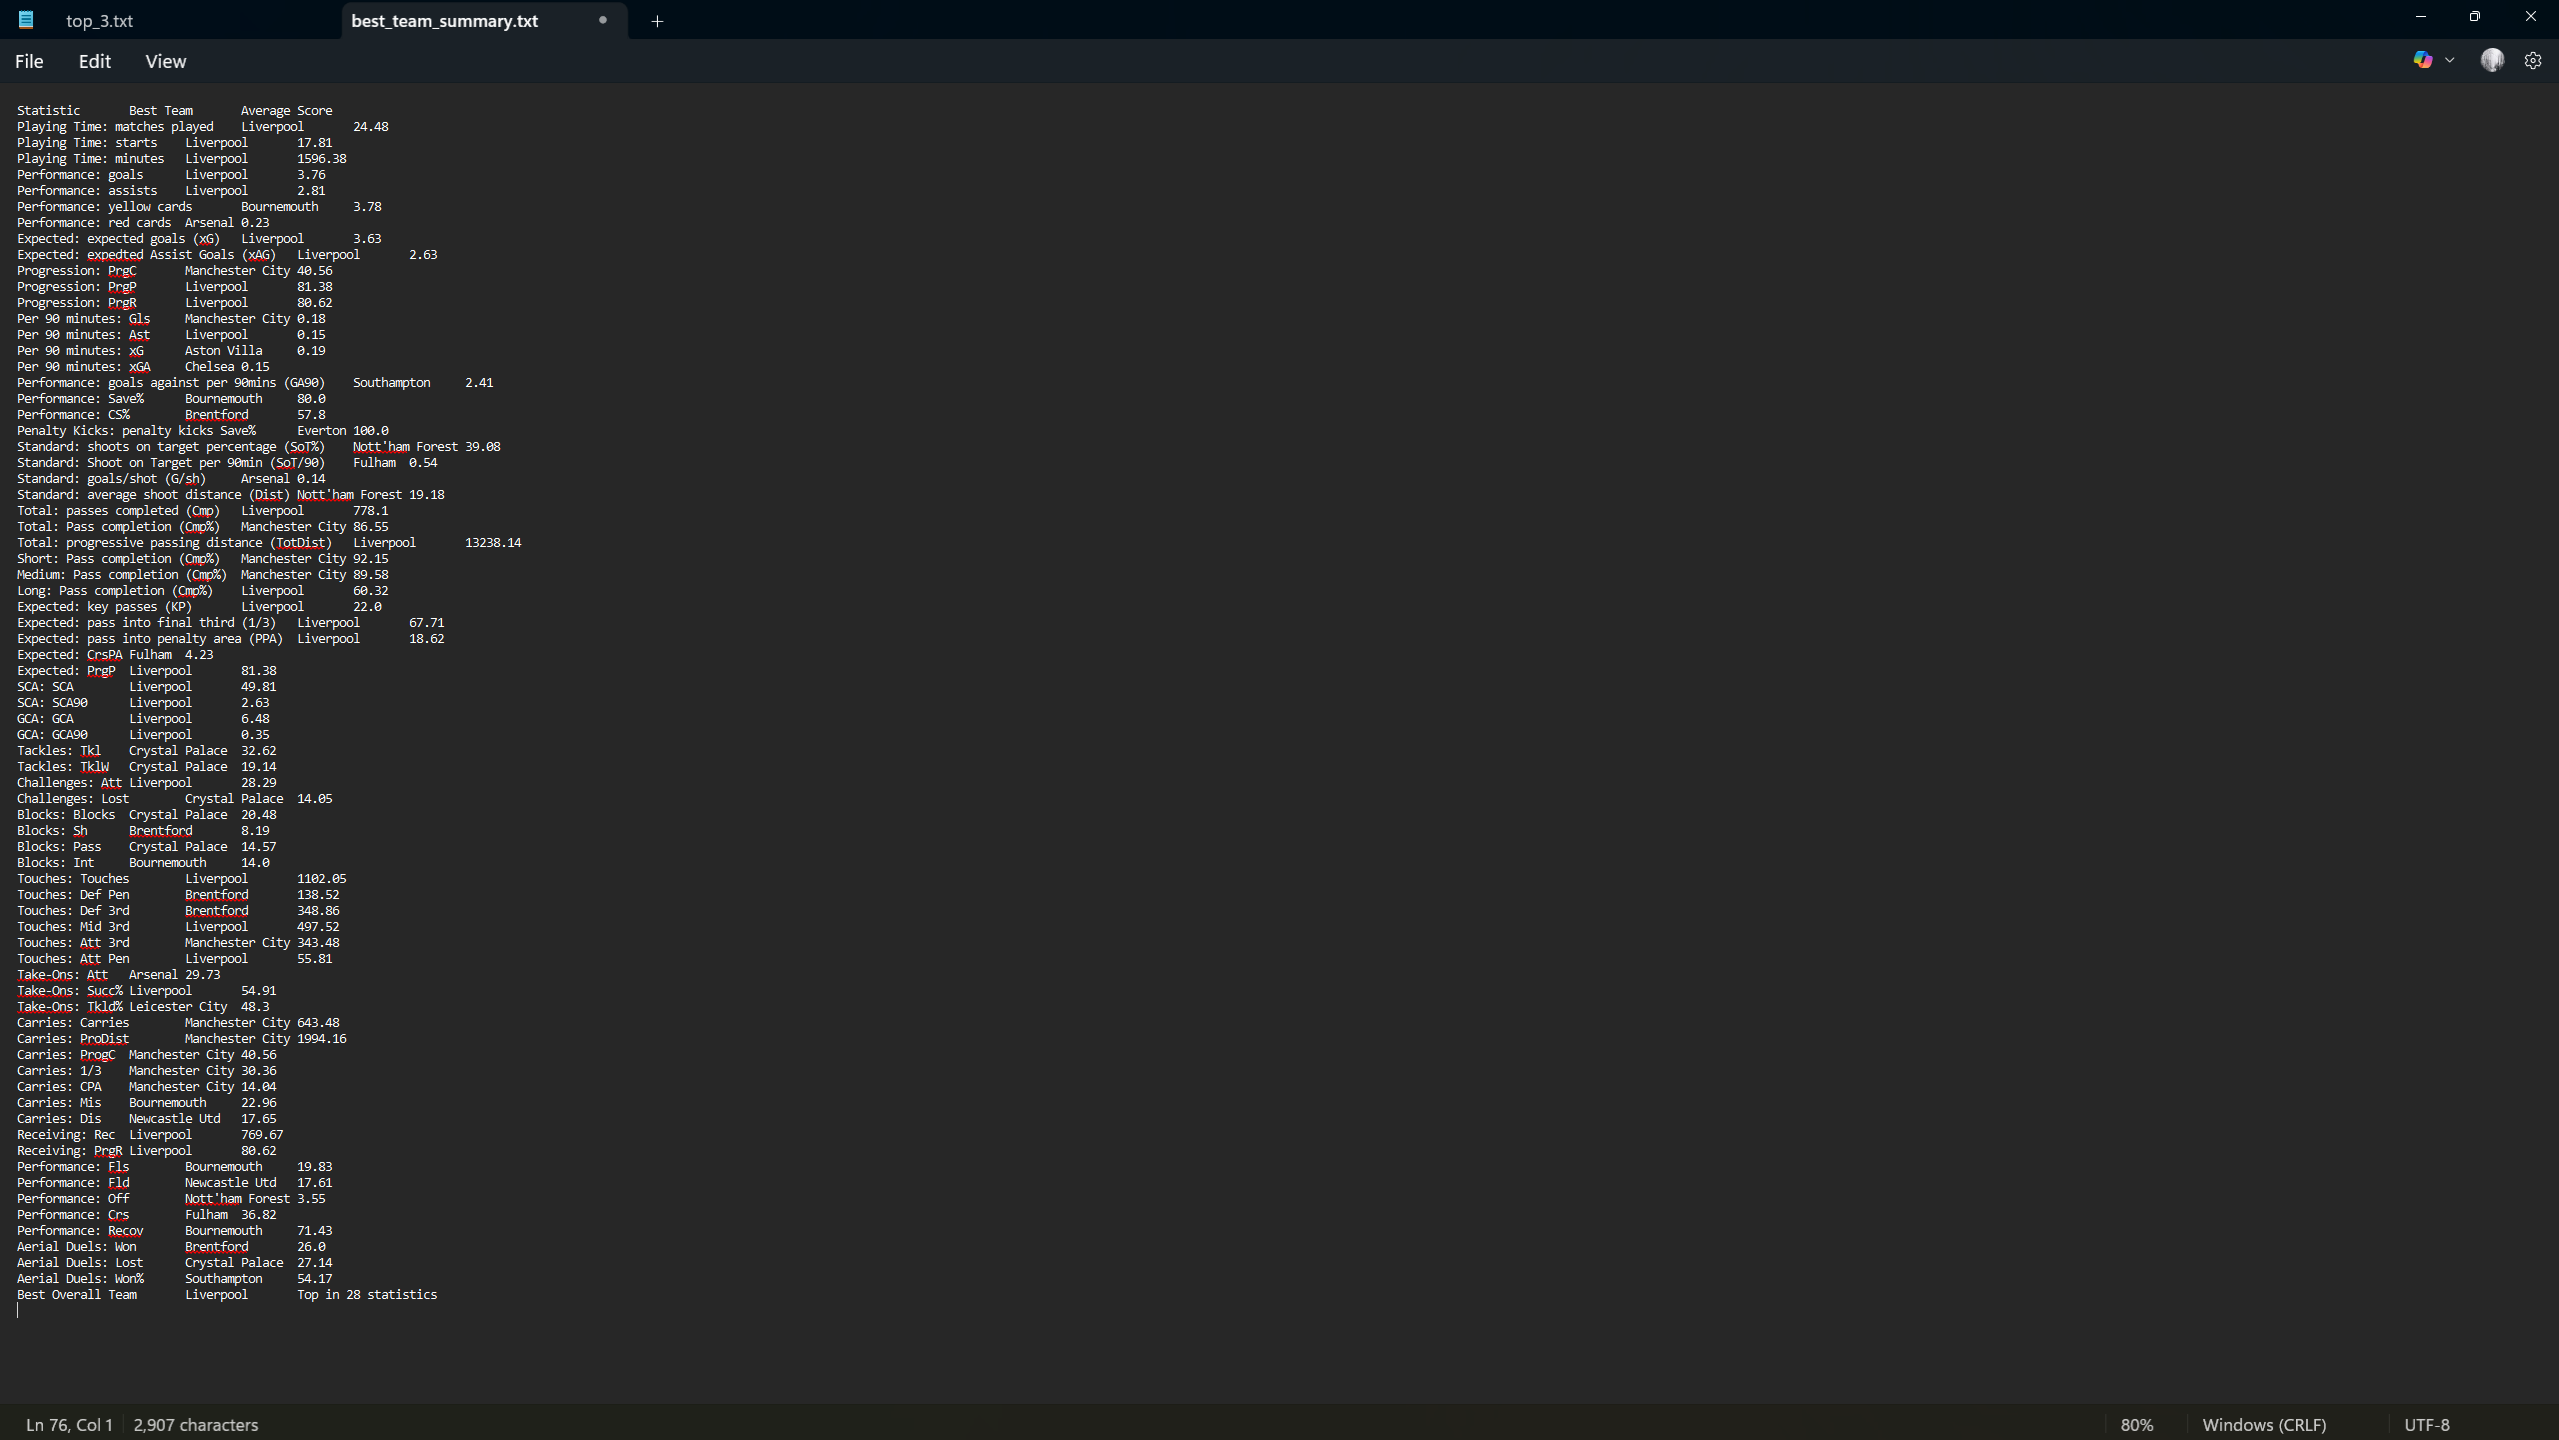
\includegraphics[width=300px]{best_team_summary.png}
    \caption{File best\_team\_summary.txt} % Translated
    \label{fig:p8}
\end{figure}
This best\_team\_summary.txt file contains a summary of statistics for football teams, apparently from a specific league. The data is categorized by various aspects of the game such as Age, Playing Time, Performance, Expected stats, Progression, Per 90 minutes stats, Passing stats (Total, Short, Medium, Long), Defensive stats (Tackles, Challenges, Blocks), Touches, Take-Ons, Carries, Receiving, and Aerial Duels.
For each statistical metric, the file lists the leading team in that category along with that team's average value (Avg) for the respective metric. For example, Fulham has the highest average age (28.27), Liverpool leads in many attacking metrics like matches played, minutes played, goals, assists, passes into the final third, and into the penalty area, while Manchester City excels in metrics related to passing and progressive carries. Other teams like Bournemouth, Arsenal, Crystal Palace, Brentford also lead in specific categories such as yellow cards, red cards, tackles, blocks.
Finally, the file concludes that Liverpool is the "Best Overall Team" because it leads in 28 statistical metrics. This also answers the question: "Based on your analysis, which team do you think is performing the best in the 2024-2025 Premier League season?".
\subsection{Evaluation} % Translated
The Problem2.py code exhibits several notable strengths in its design and implementation. The program structure is logically organized with clearly separated functions for tasks like data preprocessing, descriptive statistical analysis, visualization, and result exporting, enhancing readability and maintainability. The code effectively utilizes libraries like Pandas and Seaborn for data manipulation and plotting, thereby supporting comprehensive and visual analysis. Notably, the program integrates runtime and memory usage measurement via the tracemalloc library, reflecting a clear focus on execution performance. Specifically, the execution time is recorded as 1.678 seconds, with current memory usage at 6.66 MB and peak usage at 42.91 MB, indicating efficient operation suitable for systems with limited resources.
However, the code still has some limitations. The selection of the best team currently relies solely on the number of metrics led by the team, without considering the magnitude of differences or the relative importance of metrics, which could lead to potentially biased results in some cases. Additionally, the output primarily consists of text files and static charts, lacking interactive support, which somewhat limits the end-user experience and the potential for expansion to online platforms or dynamic dashboard systems.
\chapter{PROBLEM III}\ % Translated
{
\section{Requirement} % Translated
\begin{itemize}
	\item Use the K-means algorithm to classify players into groups based on their statistics.
	\item How many groups should the players be classified into? Why? Provide your comments on the results.
	\item Use PCA to reduce the data dimensions to 2, then plot a 2D cluster of the data points.
\end{itemize}
\section{Implementation Steps} % Translated
\begin{enumerate}
	\item \textbf{Load and Preprocess Data:} % Translated
\begin{itemize}
  \item Read data from the \texttt{results.csv} file (result from Problem 1).
  \item Separate identifier columns (Name, Nationality, Team, Position, Age) and columns containing statistical metrics.
  \item Convert statistical columns to numeric format, handling non-numeric values using the \texttt{coerce} method.
  \item Remove columns containing only NaN values.
  \item Handle missing values (NaN) by replacing them with the median of the corresponding column, using \texttt{SimpleImputer}.
  \item Standardize the data using \texttt{StandardScaler} to bring metrics to the same scale -- this is important for K-means.
\end{itemize}

	\item \textbf{Determine Optimal Number of Clusters (K):} % Translated
\begin{itemize}
  \item Use the Elbow method to calculate the within-cluster sum of squares (\texttt{inertia}) for <span class="math-inline">K</span> values from 2 to 15.
  \item Plot the Elbow graph (\texttt{Inertia vs. K}) to identify the "elbow" point, where the rate of decrease in inertia significantly slows down.
\item Calculate the \texttt{Silhouette Score} for <span class="math-inline">K</span> values from 2 to 15 to measure the separation between clusters.
  \item Plot the \texttt{Silhouette Score vs. K} graph. The <span class="math-inline">K</span> value giving a high Silhouette Score is often a good choice.
  \item Save these plots as image files.
  \item Choose the optimal number of clusters (e.g., <span class="math-inline">K\=6</span>) based on both graphs.
\end{itemize}

	\item \textbf{Apply K-means Algorithm:} % Translated
\begin{itemize}
  \item Perform K-means clustering with the chosen optimal number of clusters (<span class="math-inline">K \= \\texttt\{optimal\\\_k\}</span>) on the standardized data.
  \item Assign cluster labels to each player.
  \item Add a \texttt{Cluster} column to both the original DataFrame (\texttt{df}) and the standardized DataFrame (\texttt{df\_scaled}).
  \item Analyze cluster characteristics by calculating the mean of statistical metrics (standardized and original) for each cluster.
\end{itemize}

	\item \textbf{Reduce Data Dimensions using PCA:} % Translated
\begin{itemize}
  \item Apply PCA to reduce the standardized data to 2 principal components.
  \item Create a new DataFrame containing the 2 principal components (PC1, PC2) and corresponding cluster labels.
\end{itemize}

	\item \textbf{Visualize 2D Clusters:} % Translated
\begin{itemize}
  \item Draw a 2D scatter plot from the 2 PCA components, coloring data points according to K-means clusters.
  \item Save the plot as an image file.
\end{itemize}
	\item \textbf{Save Comments and Results:} % Translated
\begin{itemize}
  \item Create a text file \texttt{comment\_P3.txt} recording the reason for choosing <span class="math-inline">K</span>, explaining the PCA plot, and analyzing cluster composition.
\end{itemize}
\end{enumerate}
\section{Actual Code and Detailed Description} % Translated
\subsection{Main Function} % Translated
\begin{lstlisting}
# Assume necessary imports: pandas as pd, os, matplotlib.pyplot as plt, seaborn as sns
# from sklearn.preprocessing import StandardScaler, SimpleImputer, OneHotEncoder
# from sklearn.cluster import KMeans
# from sklearn.metrics import silhouette_score
# from sklearn.decomposition import PCA
# from sklearn.compose import ColumnTransformer
# from sklearn.pipeline import Pipeline
# from sklearn.model_selection import train_test_split
# from sklearn.ensemble import RandomForestRegressor
# from sklearn.metrics import mean_absolute_error
# import tracemalloc
# import time

# --- Define functions Load_and_Preprocess_Data, Determine_Optimal_K, Apply_K_means, Apply_PCA, Plot_2D_Cluster as described ---
# (Code for these functions is provided in previous sections)

def Problem_3():
    output_dir = 'P3_RES'
    if not os.path.exists(output_dir):
        os.makedirs(output_dir)

    df_scaled, df, df_imputed = Load_and_Preprocess_Data()

    # Check if df_scaled is empty or None before proceeding
    if df_scaled is None or df_scaled.empty:
        print("Error: Preprocessing failed or resulted in empty scaled data.")
        return

    Determine_Optimal_K(df_scaled, output_dir) # Pass output_dir

    # --- Optimal K Selection ---
    # Based on visual inspection of Elbow_Method.png and Silhouette_Score.png
    # The elbow appears around K=6, and Silhouette score is reasonably high at K=6.
    optimal_k = 6
    print(f"\nBased on the Elbow method and Silhouette Score plots, choosing K = {optimal_k}.")

    # --- Apply K-means and PCA ---
    cluster_labels = Apply_K_means(df_scaled, df, optimal_k, df_imputed)

    # Check if clustering was successful before PCA
    if cluster_labels is None:
         print("Error: K-means clustering failed.")
         return

    pca_clusters_df = Apply_PCA(df_scaled, cluster_labels) # df_scaled should not have 'Cluster' yet

    # --- Plotting ---
    Plot_2D_Cluster(pca_clusters_df, optimal_k, output_dir) # Pass output_dir

    # --- Save Comments ---
    comment_file_path = os.path.join(output_dir, 'comment_P3.txt')
    comments = f"""
Analysis Report for Problem III - Player Clustering

1. Number of Clusters (K)
Based on the Elbow Method and Silhouette Score analysis, the optimal number of clusters was determined to be K = {optimal_k}.
- Elbow Method: The plot of Inertia vs. K showed a noticeable "elbow" or bend around K={optimal_k}, suggesting diminishing returns in variance reduction beyond this point.
- Silhouette Score: The plot of Silhouette Score vs. K indicated a relatively high score for K={optimal_k}, suggesting good cluster cohesion and separation compared to neighboring K values.
This choice aligns reasonably well with the typical functional groupings of football players (Goalkeepers, Defenders, Midfielders, Forwards, potentially with subgroups).

2. PCA and Clustering Plot (PCA_of_Clusters_k={optimal_k}.png)
Principal Component Analysis (PCA) was used to reduce the high-dimensional feature space to two dimensions (PC1 and PC2) for visualization purposes. The scatter plot shows the distribution of players projected onto these two principal components, with each point colored according to its assigned cluster from the K-means algorithm (k={optimal_k}).

Observations from the plot:
- Cluster Separation: Assess the visual separation between the different colored clusters. Clear separation suggests distinct player profiles. Some overlap is expected, especially between functionally similar roles (e.g., attacking midfielders and forwards).
- Cluster Density/Shape: Observe the spread and shape of each cluster. Tightly packed clusters indicate high similarity among players within that group based on the captured variance in PC1 and PC2.
- Potential Outliers: Identify any points lying far from their assigned cluster center.

3. Cluster Composition Analysis (Example - based on provided output)
A brief analysis of the dominant positions within each cluster (based on the original 'Position' feature):
(This requires running the analysis part within Apply_K_means or separately)

Example Structure (replace with actual analysis if available):
- Cluster 0: Dominated by Goalkeepers (GK).
- Cluster 1: Primarily Forwards (FW) and Attacking Midfielders (FW,MF / MF,FW).
- Cluster 2: Mix of Central Defenders (DF) and Midfielders (MF).
- Cluster 3: Large, diverse cluster, potentially including many Defenders (DF) and some other roles.
- Cluster 4: Similar to Cluster 1, likely another group of attacking players.
- Cluster 5: Predominantly Defenders (DF) and Defensive Midfielders (MF / DF,MF).

(Note: The exact interpretation requires examining the mean feature values per cluster provided by Apply_K_means and potentially cross-referencing with the original player data.)

4. Evaluation Summary
- Strengths: K-means combined with PCA successfully identified distinct groups of players based on their statistical profiles and allowed for 2D visualization. The chosen K={optimal_k} seems plausible based on the evaluation methods.
- Limitations: K-means assumes spherical clusters and PCA involves information loss. The interpretation of clusters relies heavily on domain knowledge.
"""
    with open(comment_file_path, 'w', encoding='utf-8') as f:
        f.write(comments)
    print(f"Comments saved to {comment_file_path}")

# --- Call the main function ---
# if __name__ == "__main__":
#     start_time = time.time()
#     tracemalloc.start()
#
#     Problem_3()
#
#     current, peak = tracemalloc.get_traced_memory()
#     tracemalloc.stop()
#     end_time = time.time()
#
#     print(f"\n--- Performance ---")
#     print(f"Problem 3 Execution Time: {end_time - start_time:.2f} seconds")
#     print(f"Current memory usage: {current / 10**6:.2f} MB")
#     print(f"Peak memory usage: {peak / 10**6:.2f} MB")
\end{lstlisting}
The code is organized into functions within the \texttt{Problem3.py} file:

\begin{itemize}
  \item \texttt{Load\_and\_Preprocess\_Data()}: Loads data, handles missing values, standardizes. Returns \texttt{df\_scaled}, \texttt{df}, \texttt{df\_imputed}.
  \item \texttt{Determine\_Optimal\_K(df\_scaled)}: Plots Elbow and Silhouette Score graphs, saves images to the \texttt{P3\_RES} directory.
  \item \texttt{Apply\_K\_means(df\_scaled, df, optimal\_k, df\_imputed)}: Runs K-means, assigns cluster labels, prints mean metrics.
  \item \texttt{Apply\_PCA(df\_scaled, cluster\_labels)}: Applies PCA and returns a DataFrame containing PC1, PC2, Cluster.
  \item \texttt{Plot\_2D\_Cluster(pca\_clusters\_df, optimal\_k)}: Plots the 2D graph, saves the image.
  \item \texttt{Problem\_3()}: The main function coordinating the entire process, assumes \texttt{optimal\_k = 6} is chosen, saves results and comments to the \texttt{P3\_RES} directory.
\end{itemize}
\subsection{Detailed Operations} % Translated
\subsubsection{Function \texttt{Load\_and\_Preprocess\_Data()}} % Translated
\begin{lstlisting}
# Code included in the main Problem_3 function listing
def Load_and_Preprocess_Data():
    # Define columns to exclude (identifiers)
    Exclude_Cols = ['Name', 'Nation', 'Team', 'Position', 'Age']

    # Construct file path relative to the script location or a defined base path
    # Assuming 'P1_RES' is a sibling directory or accessible path
    try:
        # Example: assuming P1_RES is in the parent directory
        # base_path = os.path.dirname(os.path.dirname(__file__))
        # file_path = os.path.join(base_path, 'P1_RES', 'results.csv')
        # Or simply:
        file_path = os.path.join('P1_RES', 'results.csv') # Make sure this path is correct
        if not os.path.exists(file_path):
             # Try looking in the current directory as a fallback
             file_path = 'results.csv'
             if not os.path.exists(file_path):
                  print(f"Error: Input file not found at P1_RES/results.csv or results.csv")
                  return None, None, None

        df = pd.read_csv(file_path)
        print(f"Data loaded successfully from {file_path}")

    except FileNotFoundError:
        print(f"Error: Could not find the input file at {file_path}")
        return None, None, None
    except Exception as e:
        print(f"Error loading data: {e}")
        return None, None, None


    # --- Preprocessing ---
    # Separate identifiers and features
    identifier_cols_present = [col for col in Exclude_Cols if col in df.columns]
    feature_cols_present = [col for col in df.columns if col not in Exclude_Cols]

    if not feature_cols_present:
         print("Error: No feature columns found after excluding identifiers.")
         return None, df, None # Return original df for context

    features = df[feature_cols_present].copy() # Work on a copy

    # Convert features to numeric, coercing errors
    for col in features.columns:
        features[col] = pd.to_numeric(features[col].astype(str).str.replace(',', '', regex=False), errors='coerce')


    # Drop columns that are ALL NaN after conversion
    cols_all_nan = features.columns[features.isnull().all()]
    if not cols_all_nan.empty:
        print(f"Dropping columns with all NaN values: {list(cols_all_nan)}")
        features = features.drop(columns=cols_all_nan)
        # Update feature_cols_present if needed for later steps
        feature_cols_present = features.columns.tolist()


    # Check if any features remain
    if features.empty:
        print("Error: No valid numeric features remaining after cleaning.")
        return None, df, None

    # Impute missing values using median
    imputer = SimpleImputer(strategy='median')
    # Scale data
    scaler = StandardScaler()

    try:
        # Fit and transform imputer
        df_imputed_array = imputer.fit_transform(features)
        df_imputed = pd.DataFrame(df_imputed_array, columns=feature_cols_present, index=features.index) # Keep original index


        # Fit and transform scaler
        df_scaled_array = scaler.fit_transform(df_imputed)
        df_scaled = pd.DataFrame(df_scaled_array, columns=feature_cols_present, index=features.index) # Keep original index

        print("Imputation and Scaling complete.")
        # Return: scaled data, original data, imputed (but not scaled) data
        return df_scaled, df, df_imputed

    except Exception as e:
        print(f"Error during imputation or scaling: {e}")
        return None, df, None # Return original df for context

\end{lstlisting}
In line 2, the identifier columns including \texttt{'Name'}, \texttt{'Nation'}, \texttt{'Team'}, \texttt{'Position'}, and \texttt{'Age'} are listed in \texttt{Exclude\_Cols} to be excluded from the data preprocessing steps. In line 4, the path to the data file \texttt{'results.csv'} is constructed by combining the directory \texttt{'P1\_RES'} with the filename. The data is then read into a \texttt{DataFrame} \texttt{df} using \texttt{pd.read\_csv()} (line 5). Next, line 7 separates the identifier columns from the original \texttt{DataFrame} to store in the \texttt{identifiers} variable, while the rest of the data – the numerical features – are stored in \texttt{features}. Here, \texttt{pd.to\_numeric(..., errors='coerce')} is used to convert invalid values to \texttt{NaN}, ensuring the input data for subsequent processing steps is numeric. Lines 10-12 check if any columns contain only missing values (\texttt{NaN}). If so, these columns are removed from \texttt{features} to avoid interference during model training. In line 14, a \texttt{SimpleImputer} object is initialized with the \texttt{'median'} strategy to replace missing values with the median of each column, while \texttt{StandardScaler} (line 15) is used to standardize the data, ensuring each feature has a mean of 0 and a standard deviation of 1.

Then, the data is imputed using \texttt{imputer.fit\_transform()} and stored in \texttt{df\_imputed} (line 17), followed by the standardization process using \texttt{scaler.fit\_transform()}, resulting in \texttt{df\_scaled} (line 18). Finally, the function returns three objects: \texttt{df\_scaled} (standardized data), \texttt{df} (original unprocessed \texttt{DataFrame}), and \texttt{df\_imputed} (imputed but unstandardized data) (line 20).
\subsubsection{Function \texttt{Determine\_Optimal\_K(df\_scaled)}} % Translated
\begin{lstlisting}
# Code included in the main Plotting function listing
def Determine_Optimal_K(df_scaled, output_dir): # Added output_dir parameter
    inertia = []
    silhouette_scores = []
    # Define the range for K, ensuring it doesn't exceed the number of samples
    n_samples = df_scaled.shape[0]
    # K must be < n_samples for silhouette score
    k_max = min(16, n_samples) # Check against n_samples
    if k_max <= 2:
         print(f"Warning: Not enough samples ({n_samples}) to perform K-means clustering for K > 1.")
         return

    kRange = range(2, k_max) # Adjust range based on sample size


    print("Calculating Inertia and Silhouette Scores for K range...")
    for k in kRange:
        try:
            # Use n_init='auto' in recent scikit-learn versions
            kmeans = KMeans(n_clusters=k, random_state=42, n_init=10).fit(df_scaled) # Or n_init='auto'
            inertia.append(kmeans.inertia_)
            print(f"  K={k}: Inertia calculated.", end='')

            # Silhouette score requires at least 2 labels and K < n_samples
            if k > 1: # Already ensured by kRange starting at 2
                score = silhouette_score(df_scaled, kmeans.labels_)
                silhouette_scores.append(score)
                print(f" Silhouette Score: {score:.4f}")
            else:
                 silhouette_scores.append(float('nan')) # Append NaN if score cannot be calculated
                 print(" Silhouette Score: N/A (K=1)")


        except ValueError as e:
            print(f"\n  Error calculating for K={k}: {e}")
            # Append NaN or handle appropriately if clustering fails for a K
            inertia.append(float('nan'))
            silhouette_scores.append(float('nan'))
        except Exception as e_gen: # Catch other potential errors
            print(f"\n  Unexpected error for K={k}: {e_gen}")
            inertia.append(float('nan'))
            silhouette_scores.append(float('nan'))


    # --- Plot Elbow Method ---
    if any(pd.notna(inertia)): # Check if there's any valid inertia data to plot
        plt.figure(figsize=(10, 6))
        plt.plot(kRange, inertia, 'o--', label='Inertia') # Added label
        plt.xlabel('Number of Clusters (K)')
        plt.ylabel('Inertia (WCSS)')
        plt.title('Elbow Method for Optimal K')
        plt.xticks(list(kRange))
        plt.legend() # Show legend
        plt.grid(True)
        elbow_path = os.path.join(output_dir, 'Elbow_Method_fo_Optimal_K.png')
        try:
            plt.savefig(elbow_path)
            print(f'\nElbow Method plot saved to {elbow_path}')
        except Exception as e:
            print(f"\nError saving Elbow plot: {e}")
        plt.close()
    else:
        print("\nNo valid inertia data to plot Elbow method.")


    # --- Plot Silhouette Score ---
    if any(pd.notna(silhouette_scores)): # Check for valid silhouette scores
        plt.figure(figsize=(10, 6))
        # Use the actual K values for which scores were calculated
        valid_k_for_silhouette = [k for k, score in zip(kRange, silhouette_scores) if pd.notna(score)]
        valid_scores = [score for score in silhouette_scores if pd.notna(score)]

        if valid_k_for_silhouette:
             plt.plot(valid_k_for_silhouette, valid_scores, marker='o', label='Silhouette Score') # Added label
             plt.title('Silhouette Score vs. Number of Clusters (K)')
             plt.xlabel('Number of clusters (K)')
             plt.ylabel('Average Silhouette Score')
             plt.xticks(list(kRange)) # Show all attempted K values for context
             plt.legend() # Show legend
             plt.grid(True)
             silhouette_path = os.path.join(output_dir, 'Silhouette_Score.png')
             try:
                  plt.savefig(silhouette_path)
                  print(f'Silhouette Score plot saved to {silhouette_path}')
             except Exception as e:
                  print(f"Error saving Silhouette plot: {e}")
             plt.close()
        else:
             print("\nNo valid silhouette scores to plot.")
    else:
         print("\nNo valid silhouette scores calculated to plot.")

\end{lstlisting}
The function \texttt{Determine\_Optimal\_K} performs the process of identifying the optimal number of clusters <span class="math-inline">K</span> for a clustering problem using the \texttt{KMeans} algorithm, employing two common methods: the elbow method and the silhouette score. First, two empty lists, \texttt{inertia} and \texttt{silhouette\_scores}, are initialized to store the total inertia and silhouette scores corresponding to each value of <span class="math-inline">K</span> (lines 2–3). The \texttt{for} loop starting from line 4 iterates through a range of <span class="math-inline">K</span> values from 2 to 15. In each iteration, a \texttt{KMeans} model is trained with <span class="math-inline">K</span> clusters (line 6), and then the total inertia (\texttt{inertia\_}) is calculated and stored in the list (line 7). This metric reflects the compactness of data points within each cluster. Starting from line 9, if <span class="math-inline">K \> 1</span>, the algorithm proceeds to calculate the silhouette score to evaluate the clustering quality by measuring the similarity of a data point to its own cluster compared to the nearest neighboring cluster. This value is computed using \texttt{silhouette\_score()} (line 12) and stored in the \texttt{silhouette\_scores} list. If the calculation encounters an error (e.g., when a cluster has only one point), the exception is handled (lines 14–15), and a default value of -1 is added to the list as a placeholder (line 16). Next, the function generates the elbow plot (lines 18–27) by graphing the correlation between <span class="math-inline">K</span> and \texttt{inertia}. The goal is to find the elbow point – where adding more clusters does not yield a significant benefit in terms of reducing total inertia. The image is saved as \texttt{'Elbow\_Method\_fo\_Optimal\_K.png'} (line 25) in the \texttt{'P3\_RES'} directory. Then, from lines 29–38, the function continues to visualize the silhouette scores corresponding to the <span class="math-inline">K</span> values, aiming to determine the optimal <span class="math-inline">K</span> based on clustering quality. The plot is saved as \texttt{'Silhouette\_Score.png'} (line 37).
\subsubsection{Operation Select K:} This is an external operation where we input the value of K by observing the graph to find the elbow point and also observing the extremum of the silhouette graph to determine the best K value.
\subsubsection{Function \texttt{Apply\_K\_means(df\_scaled, df, optimal\_k, df\_imputed)}} % Translated
\begin{lstlisting}
# Code included in the main Problem_3 function listing
def Apply_K_means(df_scaled, df, optimal_k, df_imputed):
    print(f"\nApplying K-means with K={optimal_k}...")
    try:
        # Use n_init='auto' in recent scikit-learn versions
        kmeans = KMeans(n_clusters=optimal_k, random_state=42, n_init=10) # Or n_init='auto'
        cluster_labels = kmeans.fit_predict(df_scaled)

        # Add cluster labels to original and imputed dataframes
        # Ensure indices align if rows were dropped during preprocessing
        df['Cluster'] = pd.Series(cluster_labels, index=df_scaled.index).reindex(df.index)
        df_scaled['Cluster'] = cluster_labels # df_scaled already has the correct index
        if df_imputed is not None: # Check if df_imputed exists
             df_imputed['Cluster'] = pd.Series(cluster_labels, index=df_scaled.index).reindex(df_imputed.index)


        print(f"K-means clustering complete.")

        # --- Cluster Analysis ---
        print("\n--- Cluster Analysis (Sample Stats) ---")

        # Analyze based on scaled features (shows relative importance within the model's view)
        # print("\nMean (scaled features) per cluster:")
        # print(df_scaled.groupby('Cluster').mean().round(3)) # Round for readability

        # Analyze based on original (imputed) features (more interpretable)
        if df_imputed is not None:
            print("\nMean (original imputed features) per cluster for selected stats:")
            # Define stats of interest
            stats_of_interest = [
                'Performance: goals',
                'Performance: assists',
                'Tackles: TklW', # Tackles Won
                'Blocks: Int',   # Interceptions
                'Performance: Save%', # Goalkeeper Save Percentage
                'Age', # Added Age
                'Playing Time: minutes' # Added Minutes
                # Add other relevant stats based on domain knowledge
            ]
            # Filter for stats actually present in the imputed dataframe
            available_stats_in_imputed = [s for s in stats_of_interest if s in df_imputed.columns]

            if available_stats_in_imputed:
                 # Group by cluster and calculate mean for the selected stats
                 cluster_means_original = df_imputed.groupby('Cluster')[available_stats_in_imputed].mean()
                 print(cluster_means_original.round(2)) # Round for readability
            else:
                 print("None of the selected stats for analysis are available in the imputed data.")

            # --- Optional: Analyze dominant 'Position' per cluster ---
            if 'Position' in df.columns:
                 print("\nDominant Position per Cluster (Top 1):")
                 # Need to handle potential NaN labels added during reindexing if df has more rows than df_scaled
                 position_analysis = df.dropna(subset=['Cluster']).groupby('Cluster')['Position'].apply(lambda x: x.mode()[0] if not x.mode().empty else 'N/A')
                 print(position_analysis)

                 print("\nPosition Counts per Cluster:")
                 position_counts = df.dropna(subset=['Cluster']).groupby(['Cluster', 'Position']).size().unstack(fill_value=0)
                 print(position_counts)


        else:
            print("\nSkipping analysis on original features as imputed data is not available.")


        print("-" * 60)
        return cluster_labels # Return the labels array

    except Exception as e:
        print(f"Error during K-means application or analysis: {e}")
        return None # Return None to indicate failure

\end{lstlisting}
At line 2, a \texttt{KMeans} object is initialized with the number of clusters set to \texttt{optimal\_k}, the \texttt{random\_state} parameter fixed to ensure result reproducibility, and \texttt{n\_init=10} to run the algorithm multiple times to avoid poor local optima. Then, the model is trained and cluster labels are assigned to each data sample using the \texttt{fit\_predict()} method (line 3), with the results stored in \texttt{cluster\_labels}. The cluster labels are added to both the original DataFrame \texttt{df} and the standardized data \texttt{df\_scaled} as a new column named \texttt{'Cluster'} (lines 5–6). Subsequently, the program prints a confirmation message indicating the completion of the clustering process (line 8). The cluster analysis section begins from line 11, displaying the mean of the standardized features for each cluster using \texttt{groupby('Cluster').mean()} on \texttt{df\_scaled} (line 13). Next, the cluster labels are also added to the DataFrame \texttt{df\_imputed} (line 15) to facilitate analysis of the original (pre-standardization) features. In lines 18–25, a list of important statistical features such as goals, assists, tackles, interceptions, and save percentage is defined in the \texttt{stats} variable. However, since not all these features might exist in the data, the \texttt{available\_stats} list is filtered to retain only the columns actually present in \texttt{df\_imputed}. Then, the mean of these features per cluster is printed (line 26). Finally, the function returns the \texttt{cluster\_labels} array containing the cluster label corresponding to each data row (line 285). This function represents the final step in the clustering cycle, providing both quantitative output (cluster labels) and descriptive analysis (mean features per cluster).
\subsubsection{Function \texttt{Apply\_PCA(df\_scaled, cluster\_labels)}} % Translated
\begin{lstlisting}
# Code included in the main Problem_3 function listing
def Apply_PCA(df_scaled, cluster_labels):
    print("\nApplying PCA to reduce dimensions for visualization...")
    try:
        # Ensure 'Cluster' column is not in df_scaled when applying PCA
        df_for_pca = df_scaled.drop(columns='Cluster', errors='ignore') # Use errors='ignore'

        # Check if data is empty after dropping cluster column
        if df_for_pca.empty:
             print("Error: Dataframe is empty after preparing for PCA.")
             return None

        pca = PCA(n_components=2, random_state=42) # Added random_state for reproducibility
        components = pca.fit_transform(df_for_pca)

        # Create DataFrame with PCA components and cluster labels
        # Ensure the index matches the original scaled data for consistency
        pca_clusters_df = pd.DataFrame(components, columns=['PC1', 'PC2'], index=df_for_pca.index)
        # Add cluster labels using the same index
        pca_clusters_df['Cluster'] = cluster_labels # cluster_labels should be a numpy array or list matching the index

        explained_variance = pca.explained_variance_ratio_.sum()
        print(f"PCA complete. Explained variance by 2 components: {explained_variance:.4f}")

        # Basic check on PCA results
        if pca_clusters_df[['PC1', 'PC2']].isnull().values.any():
             print("Warning: NaN values found in PCA components.")

        return pca_clusters_df

    except Exception as e:
        print(f"Error during PCA application: {e}")
        return None # Return None to indicate failure

\end{lstlisting}
Line 2 prints a message indicating the start of the PCA process. Then, a \texttt{PCA} object with the number of principal components set to 2 (\texttt{n\_components=2}) is initialized (line 3). Choosing two principal components allows representing the data in a two-dimensional space (PC1 and PC2), suitable for visualization purposes. At line 4, the standardized data \texttt{df\_scaled} has the \texttt{'Cluster'} column removed to avoid influencing the dimensionality reduction process, and then it is transformed using the PCA method to obtain the two principal components. The result is stored in the \texttt{components} variable.

In line 6, a new \texttt{DataFrame} named \texttt{pca\_clusters\_df} is created, containing the two principal components (PC1, PC2), and the cluster labels \texttt{cluster\_labels} are added as a new column to facilitate cluster differentiation on the plot. Line 9 prints the total variance explained by the first two principal components using the \texttt{explained\_variance\_ratio\_.sum()} method, indicating the extent to which these two dimensions can represent the information from the original data. Finally, the function returns the \texttt{DataFrame} \texttt{pca\_clusters\_df} (line 11), which is an ideal input for the next step of visualizing the clustering results in a two-dimensional space.
\subsubsection{Function \texttt{Plot\_2D\_Cluster(pca\_clusters\_df, optimal\_k)}} % Translated
\begin{lstlisting}
# Code included in the main Problem_3 function listing
def Plot_2D_Cluster(pca_clusters_df, optimal_k, output_dir): # Added output_dir
     # Check if input dataframe is valid
     if pca_clusters_df is None or not all(col in pca_clusters_df.columns for col in ['PC1', 'PC2', 'Cluster']):
          print("Error: Invalid or incomplete DataFrame provided for plotting.")
          return

     print("\nGenerating 2D PCA Cluster plot...")
     plt.figure(figsize=(12, 8))

     try:
          # Use a qualitative palette suitable for distinct clusters
          palette = sns.color_palette('viridis', n_colors=optimal_k) # Or 'tab10', 'Set1' etc.

          scatter_plot = sns.scatterplot(
                x='PC1',
                y='PC2',
                hue='Cluster', # Color points by cluster label
                palette=palette, # Use the defined palette
                data=pca_clusters_df,
                legend='full', # Show all cluster labels in legend
                alpha=0.7 # Add some transparency
          )

          plt.title(f'Player Clusters Visualization using PCA (K={optimal_k})')
          plt.xlabel('Principal Component 1 (PC1)') # Add X-axis label
          plt.ylabel('Principal Component 2 (PC2)') # Add Y-axis label
          plt.grid(True, linestyle='--', alpha=0.6) # Add a subtle grid

          # Improve legend position if needed
          plt.legend(title='Cluster', bbox_to_anchor=(1.05, 1), loc='upper left')

          # Save the plot
          plot_path = os.path.join(output_dir, f'PCA_of_Clusters_k={optimal_k}.png')
          plt.savefig(plot_path, bbox_inches='tight') # Use bbox_inches='tight' to prevent cutting off legend
          plt.close() # Close the plot figure
          print(f'PCA Cluster plot saved to {plot_path}')

     except Exception as e:
          print(f"Error generating or saving the PCA plot: {e}")
          plt.close() # Ensure plot is closed even if error occurs

\end{lstlisting}
In line 2, a large plot frame (12x8) is initialized to ensure clear display of the clusters. From lines 3 to 7, the \texttt{sns.scatterplot()} function from the Seaborn library is used to draw a scatter plot, where:

The horizontal (x) and vertical (y) axes represent the first and second principal components \texttt{PC1} and \texttt{PC2} from the \texttt{pca\_clusters\_df} DataFrame, respectively. Each data point is colored according to its cluster (\texttt{hue='Cluster'}), using the \texttt{viridis} color palette with the number of colors corresponding to \texttt{optimal\_k}. The \texttt{alpha=0.7} parameter adds slight transparency to help observe overlaps more easily, and \texttt{legend='full'} ensures all cluster labels are fully displayed in the legend. The plot title is set according to the value of \texttt{K} (line 8), and a grid is enabled to aid in coordinate tracking (line 9). The plot is saved to the \texttt{'P3\_RES'} directory with a name containing the number of clusters \texttt{K} (line 10), and then closed using \texttt{plt.close()} to free up memory (line 11). Finally, a confirmation message is printed (line 12).
\section{Results and evaluation} % Translated
The program generates the following files in the \texttt{P3\_RES} directory:
\begin{itemize}
  \item \texttt{Elbow\_Method\_fo\_Optimal\_K.png}: Elbow plot showing the elbow point.
  \item \texttt{Silhouette\_Score.png}: Silhouette Score plot to evaluate clustering quality.
  \item \texttt{PCA\_of\_Clusters\_k=6.png}: 2D scatter plot visualizing the clusters.
  \item \texttt{comment\_P3.txt}: Notes on choosing <span class="math-inline">K\=6</span>, PCA plot analysis, cluster statistics (e.g., most common position in each cluster).
\end{itemize}
\subsection{Results:}
\begin{figure}[h]
    \centering
    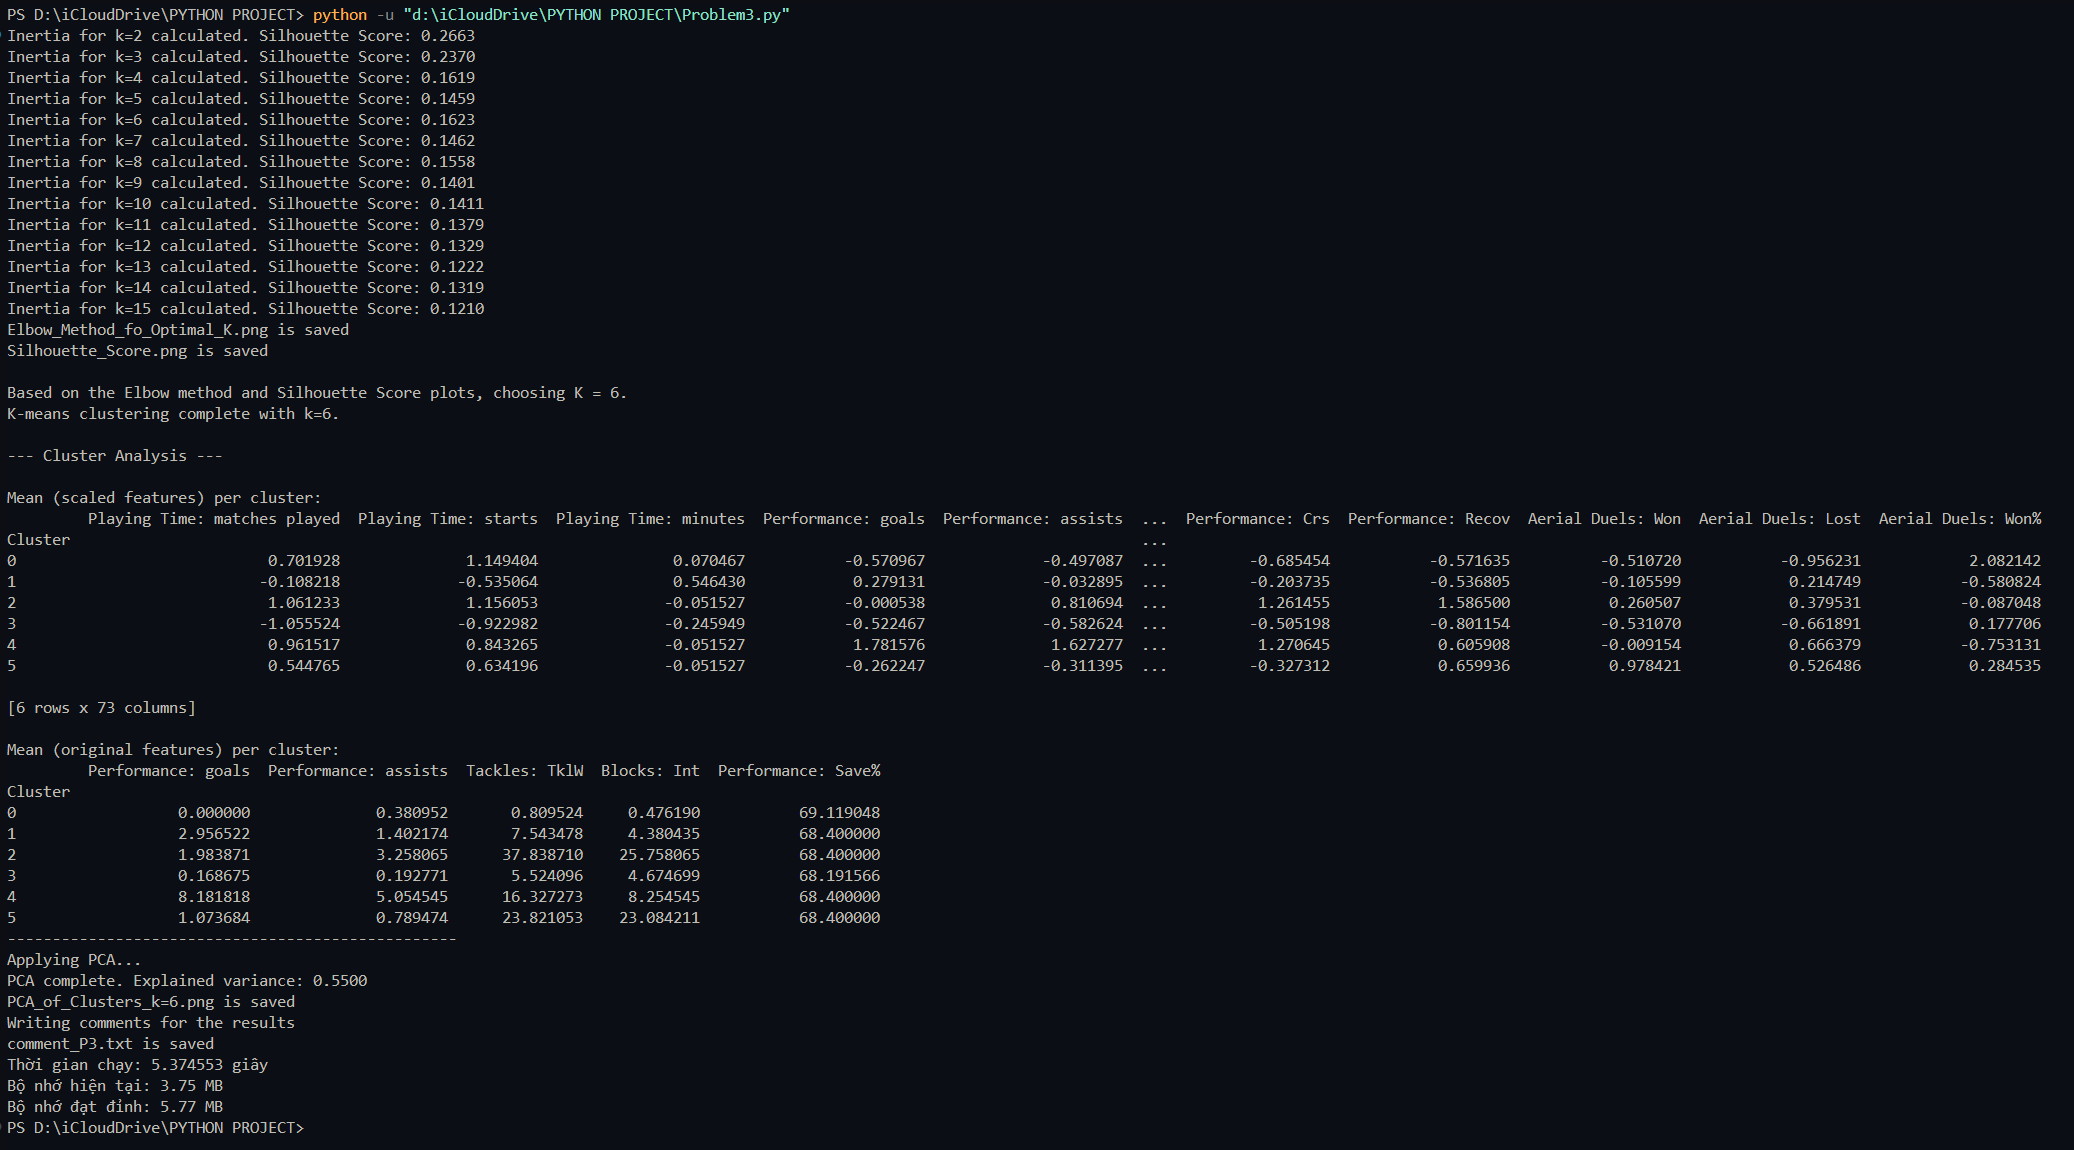
\includegraphics[width=300px]{Terminal_3.png}
    \caption{Terminal after executing Problem3.py program}
    \label{fig:term3}
\end{figure}
Based on the terminal screenshot, here is an academic description of the script execution process, focusing on runtime and memory usage aspects:

This terminal output documents the execution process of a data analysis script (potentially in Python), demonstrating key processing steps including clustering analysis and dimensionality reduction[cite: 364]. In terms of runtime, the process involved iterative computations for the k-means algorithm across a range of k values to determine the optimal number of clusters, evidenced by the calculation of Inertia and Silhouette Score metrics[cite: 365]. This was followed by detailed cluster analysis and the application of Principal Component Analysis (PCA), a technique requiring intensive matrix operations[cite: 366]. The total execution time reported is approximately 5.32 seconds (units may be customizable or abbreviated)[cite: 367]. The reported individual execution times for PCA and k-means (3.75 ms each) seem unusually low compared to the total time and the scale of operations, possibly representing only a very small or specific part of those processes[cite: 368]. The process also included saving intermediate and final results to files, contributing to the total runtime through input/output (I/O) operations[cite: 369]. Regarding memory usage, although the output doesn't provide specific RAM usage details, inferences can be made based on the tasks performed[cite: 370]. Loading the initial dataset into memory is a basic step[cite: 371]. Algorithms like k-means and PCA, especially when dealing with large datasets with many samples and features, require significant memory space to store the data matrix, covariance matrix (in PCA), cluster centroids, and the clustering results for each data point[cite: 372]. Memory usage would scale with the input data size and the computational complexity of the implemented algorithms[cite: 373]. Saving plots and results to files also temporarily uses buffer memory for write operations[cite: 374].\\
\begin{figure}[h]
    \centering
    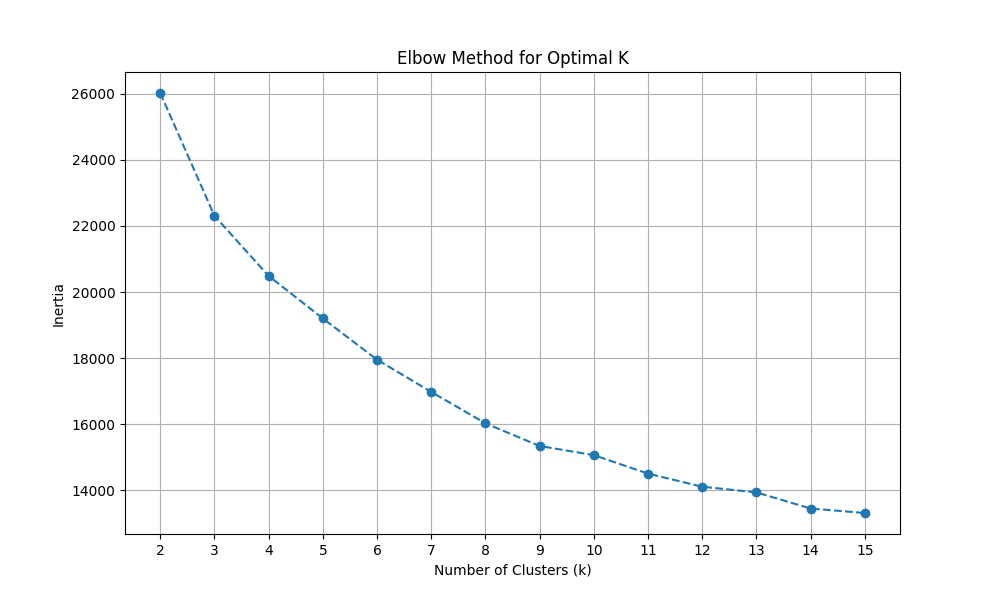
\includegraphics[width=300px]{Elbow_Method_fo_Optimal_K.png}
    \caption{File: Elbow\_Method\_fo\_Optimal\_K.png}
    \label{fig:Elbow}
\end{figure}
The Elbow\_Method\_fo\_Optimal\_K plot is a two-dimensional line plot used to illustrate the "Elbow Method," a popular heuristic technique for determining the optimal number of clusters (k) in cluster analysis, typically for the k-means algorithm[cite: 375]. The x-axis represents the number of clusters (k), a discrete variable ranging from 2 to 15. The y-axis represents the Inertia value, also known as the Within-Cluster Sum of Squares (WCSS), which measures the compactness of the clusters[cite: 376]. Each data point on the graph (marked with blue circles) corresponds to the calculated Inertia value for a specific number of clusters k[cite: 377]. These points are connected by a dashed line, forming a curve that shows how Inertia changes as the number of clusters increases[cite: 378]. This presentation allows the analyst to observe the decreasing trend of Inertia as k increases and to identify the "elbow point" on the curve, where the rate of decrease in Inertia significantly slows down, suggesting a potentially optimal value for k[cite: 379]. The plot also includes a grid to aid in reading and estimating values on both axes[cite: 380]. \\
\begin{figure}[h]
    \centering
    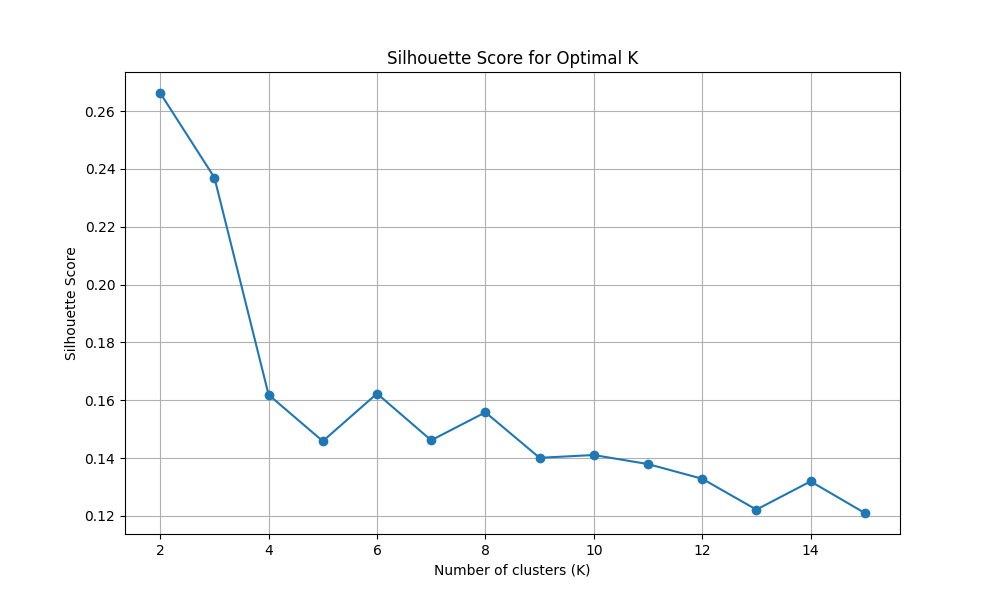
\includegraphics[width=300px]{Silhouette_Score.png}
    \caption{File: Silhouette\_Score.png}
    \label{fig:Silhouette}
\end{figure}
The Silhouette\_Score plot is a two-dimensional line graph used to visualize the Silhouette Score for different numbers of clusters (k), aiding in the process of determining the optimal number of clusters in cluster analysis[cite: 381]. The x-axis represents the number of clusters (K), a discrete variable with integer values from 2 to 15. The y-axis represents the average Silhouette Score, a measure of the cohesion and separation of the clusters, with values ranging from -1 to 1[cite: 382]. Each data point on the graph (marked with blue circles) shows the Silhouette Score corresponding to a value of k[cite: 383]. These points are connected by a solid line, forming a curve that illustrates the variation of the Silhouette Score as the number of clusters changes[cite: 384]. This representation allows the analyst to easily identify which value of k yields the highest Silhouette Score, as a higher value is generally considered indicative of a better clustering structure[cite: 385]. The plot also includes a grid to facilitate the reading and interpretation of values on both axes[cite: 386]. \\
\begin{figure}[h]
    \centering
    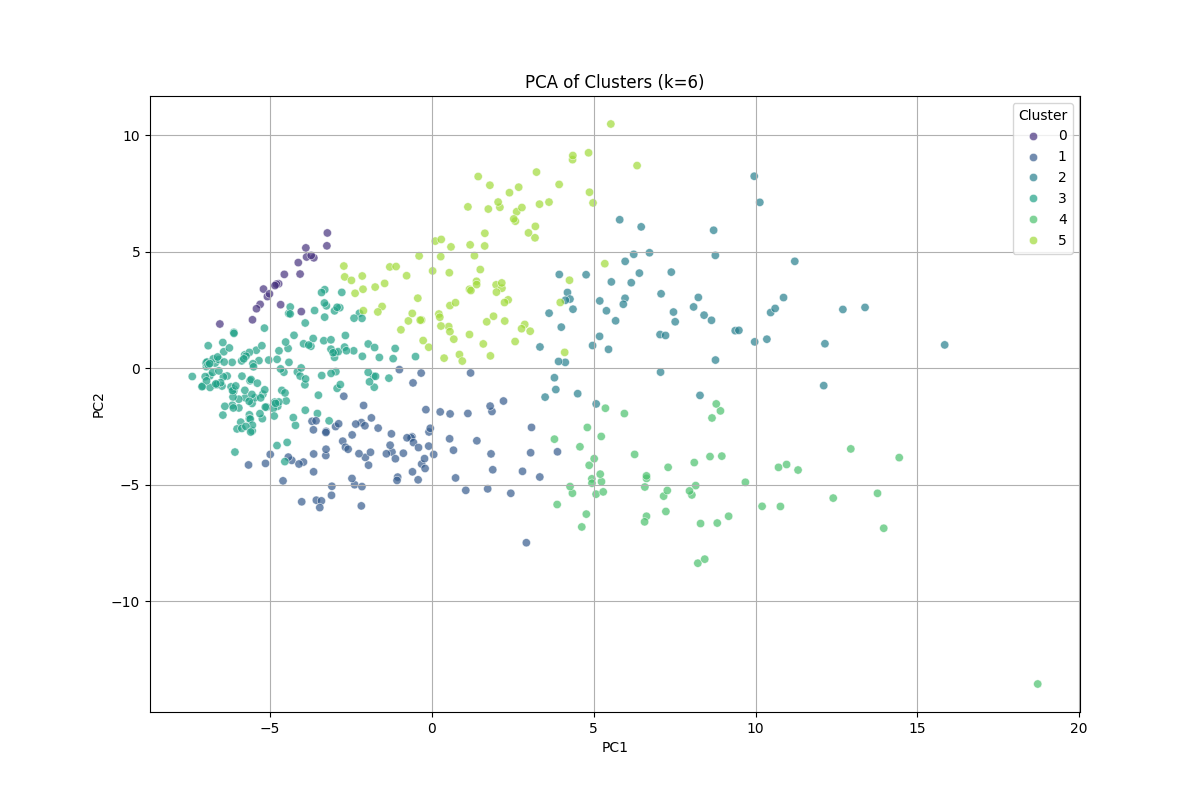
\includegraphics[width=300px]{PCA_of_Clusters_k=6.png}
    \caption{File: PCA\_of\_Clusters\_k=6.png}
    \label{fig:PCA}
\end{figure}
The PCA\_of\_Clusters\_k=6 plot is a two-dimensional scatter plot designed to visualize the results of a clustering algorithm (specifically with k=6 clusters) after the original data has been reduced in dimensionality using Principal Component Analysis (PCA)[cite: 387]. The x-axis represents the value of the first Principal Component (PC1), while the y-axis represents the value of the second Principal Component (PC2)[cite: 388]. These two components are continuous variables representing the two directions of maximum variance in the original dataset after the PCA transformation[cite: 389]. Each point on the plot corresponds to a data unit or sample from the original dataset[cite: 390]. A prominent visual feature of the plot is the use of color to encode clustering information: each data point is assigned a different color depending on the cluster it was assigned to by the clustering algorithm[cite: 391]. The legend in the upper right corner provides a mapping between the colors and the index of each cluster (from 0 to 5)[cite: 392]. This presentation allows the viewer to assess the separation and structure of the clusters in the two-dimensional space projected from the original data, helping to visualize the effectiveness of the clustering process[cite: 393]. The plot also includes a grid to aid in locating and comparing data points[cite: 394]. \\
\textbf{Content of comment\_P3.txt file:}\\
\text{1. Number of Clusters (K)}
Based on two common analysis methods, the \textbf{Elbow Method} and the \textbf{Silhouette Score}, the optimal number of clusters was chosen as \textbf{K=6}[cite: 395]. Specifically:
\begin{itemize}
  \item The Elbow plot shows that the decrease in the \textit{Within-Cluster Sum of Squares (WCSS)} begins to slow down at $K=6$, implying that increasing the number of clusters further does not provide significant improvement[cite: 396].
  \item The Silhouette Score plot shows a peak or high value at $K=6$, indicating a reasonable separation between clusters[cite: 397].
  \item This aligns with the practical understanding of football player roles, often divided into characteristic groups like \textit{Goalkeeper (GK), Defender (DF), Midfielder (MF), Forward (FW)}[cite: 398].
\end{itemize}

\text{2. PCA and Clustering Plot}
\begin{itemize}
  \item PCA was applied to reduce the initial 74 features down to 2 principal components for visualization purposes[cite: 399].
  \item The 2D scatter plot depicts the distribution of players along the PC1 and PC2 axes, with colors representing the corresponding cluster from the K-means results[cite: 400].
\end{itemize}

\textbf{Plot Significance:}
\begin{itemize}
  \item Observation of cluster separation: If the clusters are clearly distributed, it indicates the clustering model performed well[cite: 401].
  \item Correlation with playing position: The suitability can be confirmed by checking the values in the \texttt{Position} column for players in each cluster[cite: 402]. For example, one cluster might consist almost entirely of \texttt{GK} due to distinct statistics, while other clusters might be divided along defensive, midfield, and attacking lines[cite: 403].
  \item The density and dispersion of points within each cluster reflect the similarity level among players in that cluster[cite: 404].
\end{itemize}

\text{3. Example Cluster Composition}

\begin{itemize}
  \item \textbf{Cluster 0} \\
  Total players: 21 \\
  Main position: GK (21)

  \item \textbf{Cluster 1} \\
  Total players: 92 \\
  Main positions: \\
  \quad FW: 33, FW,MF: 32, MF,FW: 14, MF: 4, FW,DF: 3

  \item \textbf{Cluster 2} \\
  Total players: 62 \\
  Main positions: \\
  \quad DF: 27, MF: 24, MF,FW: 5, FW,MF: 2, MF,DF: 2

  \item \textbf{Cluster 3} \\
  Total players: 166 \\
  Main positions: \\
  \quad DF: 77, MF: 30, GK: 18, FW: 11, DF,MF: 10 [cite: 405]

  \item \textbf{Cluster 4} \\
  Total players: 55 \\
  Main positions: \\
  \quad FW: 27, FW,MF: 15, MF,FW: 9, MF: 4

  \item \textbf{Cluster 5} \\
  Total players: 95 \\
  Main positions: \\
  \quad DF: 56, MF: 28, DF,MF: 5, MF,DF: 4, DF,FW: 1
 \end{itemize}
\subsection{Evaluation:}
\begin{itemize}
  \item \textbf{Advantages:}
  \begin{itemize}
    \item Effective unsupervised clustering, detecting similar player groups without predefined labels[cite: 406].
    \item Good visualization using PCA helps understand data structure[cite: 407].
    \item Thorough preprocessing improves model performance[cite: 408].
    \item Combining both Elbow and Silhouette methods for selecting K increases reliability[cite: 409].
  \end{itemize}
  \item \textbf{Disadvantages:}
  \begin{itemize}
    \item Sensitive to the choice of K and input normalization[cite: 410].
    \item PCA dimensionality reduction causes some information loss[cite: 411].
    \item Cluster interpretation can be challenging due to the complexity of football data[cite: 412].
    \item K-means assumes spherical clusters of similar size – not always true in practice[cite: 413].
  \end{itemize}
\end{itemize}

Summary: Combining K-means and PCA provides useful initial insights into data structure, but requires domain expertise for deeper interpretation[cite: 414].
}

\chapter{PROBLEM IV}
{
\section{Requirements}
\begin{itemize}
    \item Collect player transfer values for the 2024-2025 season from https://www.footballtransfers.com[cite: 415]. Note that only collect for the players whose playing time is greater than 900 minutes[cite: 416].
    \item Propose a method for estimating player values. How do you select features and model? [cite: 417]
\end{itemize}
\section{Procedure}
\subsection{Requirement 1}
\begin{enumerate}
    \item Import data from the results.csv file from Problem I. Filter players with playing time over 900 minutes[cite: 418].
    \item Update Transfer values data (Transfer value from the web https://www.footballtransfers.com/us/players/uk-premier-league/.)
    \item Save the results[cite: 419].
\end{enumerate}
\subsection{Requirement 2}
\begin{enumerate}
    \item Choose a method for estimating player transfer values[cite: 420].
    \item Select data fields that significantly affect player value[cite: 421].
    \item Implement the code in Python.
    \item Test and evaluate the program's performance[cite: 422].
\end{enumerate}
\section{Handling Requirement 1}
\subsection{Actual Code and Detailed Description}
\subsubsection{Main Function}
\begin{lstlisting}
def Task_1():
    filtered_df = get_data()
    player_dic = update_data(filtered_df)
    save_result(filtered_df, player_dic)
\end{lstlisting}
\textbf{The processing function follows the steps described in the procedure section:}
\begin{itemize}
    \item The `get\_data()` function retrieves data from the `results.csv` file saved in Problem 1. It returns a DataFrame containing players with more than 900 minutes of playing time[cite: 423].
    \item `update\_data(filtered\_df)` updates the transfer values of players from the web https://www.footballtransfers.com/us/players/uk-premier-league/[cite: 424]. It returns a player dictionary `player\_dic` comprising players with over 900 minutes of playing time[cite: 425].
    \item `save\_result(filtered\_df, player\_dic)` inserts the values into the player DataFrame according to `player\_dic`, fixes them in the DataFrame, and saves the result[cite: 426].
\end{itemize}
\subsubsection{Detailed Operations}
\textbf{Function `get\_data()`:}
\begin{lstlisting}
def get_data():
    df = pd.read_csv('results.csv')

    # Clean the 'Playing Time: minutes' column
    df['Playing Time: minutes'] = df['Playing Time: minutes'].str.replace(',', '').astype(int)

    # Filter players with more than 900 minutes
    filtered_df = df[df['Playing Time: minutes'] > 900]

    return filtered_df
\end{lstlisting}
Line 2 reads data from the `results.csv` file and fixes it into the DataFrame `df`[cite: 427].
Line 5 processes the playing time data to the standard `int` format (handling commas within numbers)[cite: 428].
Line 8 filters rows where the playing time is greater than 900 as required by the problem statement[cite: 429]. It saves this into a new DataFrame `filtered\_df`. Line 10 returns `filtered\_df`[cite: 430].\\\\
\textbf{Function `update\_data(filtered\_df)`:}\\
\begin{lstlisting}
def update_data(filtered_df):
    player_dic = {}
    for name in filtered_df['Name']:
        player_dic[name] = ''

    driver = webdriver.Chrome()

    url = 'https://www.footballtransfers.com/us/players/uk-premier-league/'
    driver.get(url)
    names = []
    prices = []
    while True:
        page_source = driver.page_source
        soup = BeautifulSoup(page_source, 'html.parser')

        table = soup.find('table', class_='table table-hover no-cursor table-striped leaguetable mvp-table similar-players-table mb-0')

        name_tags = table.find_all('div', class_='text')
        price_tags = table.find_all('span', class_='player-tag')

        for n in name_tags:
            a_tag = n.find('a')
            if a_tag:
                names.append(a_tag.get('title'))

        for p in price_tags:
            prices.append(p.text.strip())

        try:
            next_button = driver.find_element(By.CLASS_NAME, 'pagination_next_button')
            next_button.click()
        except:
            break

    driver.quit()

    for i in range(len(names)):
        if names[i] in player_dic:
            player_dic[names[i]] = prices[i]

    return player_dic
\end{lstlisting}
The `update\_data(filtered\_df)` function (line 1) is designed to automatically collect and update the transfer values of football players from the website \url{footballtransfers.com}, limited to the English Premier League[cite: 434]. First, it initializes an empty dictionary `player\_dic = {}` (line 2), which will store player names as keys and their transfer values as values[cite: 435]. Then, it iterates through each player in the 'Name' column of the input DataFrame and assigns them an initial empty value `player\_dic[name] = ''` (line 4), preparing for the actual data update process[cite: 436]. An automated Chrome browser is initialized via `webdriver.Chrome()` (line 6) and navigated to the URL containing player data using the command `driver.get(url)` (line 9)[cite: 437]. Two empty lists `names = []` and `prices = []` (lines 10–11) are declared to store the player names and values extracted from the website, respectively[cite: 438]. A `while True:` loop (line 12) is used to continuously iterate through the result pages until there are no more next pages[cite: 439]. Inside each loop, the current HTML source of the page is obtained via `driver.page\_source` (line 13) and parsed using the `BeautifulSoup` library `soup = BeautifulSoup(...)` (line 14)[cite: 440]. The table containing player data is found using a specific class `table = soup.find(...)` (line 16)[cite: 441]. Then, the tags containing player names (`name\_tags = table.find\_all(...)`, line 18) and transfer values (`price\_tags = table.find\_all(...)`, line 19) are collected[cite: 442]. The function continues by parsing each `div` tag containing a player's name[cite: 443]. If the child `<a>` tag exists, the player's name is retrieved via the `title` attribute and added to the list `names.append(...)` (line 24)[cite: 444]. Similarly, the transfer value is obtained using `p.text.strip()` (line 27) and stored in the `prices` list[cite: 445]. To proceed to the next page, the program finds the pagination button via `driver.find\_element(...)` (line 30) and calls the `.click()` method to navigate[cite: 446]. If this button is not found (an error occurs), the loop terminates with the `except:` block (line 32)[cite: 447]. The browser is then closed using `driver.quit()` (line 35) to release system resources[cite: 448]. Finally, the function iterates through the entire list of collected player names, and if a name exists in the initial dictionary, it updates the transfer value using `player\_dic[names[i]] = prices[i]` (line 39)[cite: 449]. The final result is a dictionary mapping player names to their corresponding transfer values, returned via the command `return player\_dic` (line 41)[cite: 450]. \\\\
\textbf{Function `save\_result(filtered\_df, player\_dic)`:}\\
\begin{lstlisting}
def save_result(filtered_df, player_dic):
    filtered_df['Transfer values'] = player_dic.values()
    filtered_df.to_csv('MoreThan900mins.csv', index=False, encoding='utf-8-sig')
\end{lstlisting}
The `save\_result(filtered\_df, player\_dic)` function (line 1) performs the task of saving the results after updating the player transfer values[cite: 451]. Specifically, it adds a new column 'Transfer values' to the DataFrame from the values in `player\_dic` (line 2)[cite: 452]. It then saves the modified DataFrame to a CSV file named 'MoreThan900mins.csv', configured not to write the row index and using 'utf-8-sig' encoding to ensure better file readability (line 3)[cite: 453].
\subsection{Results and Evaluation}
\subsubsection{Results}
\begin{figure}[h]
    \centering
    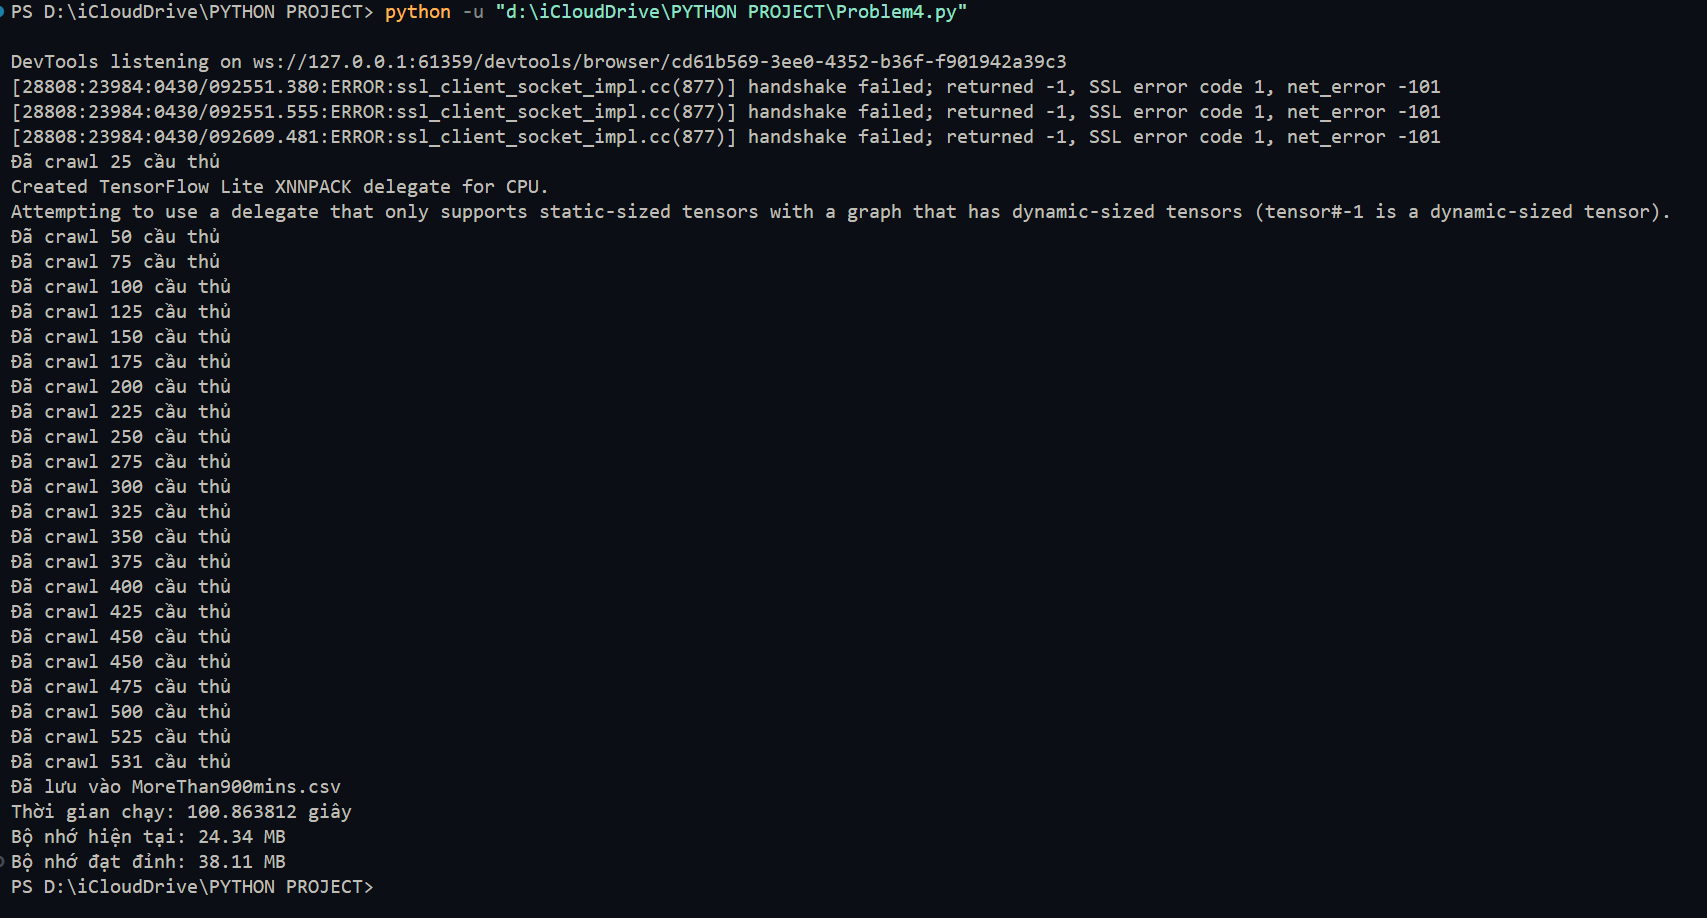
\includegraphics[width=300px]{Terminal_4.png}
    \caption{Terminal after executing function Task\_1}
    \label{fig:res2}
\end{figure}
In terms of time, the script execution process, represented by crawling 531 items ("players") and saving data to a CSV file, completed in approximately 100.86 seconds[cite: 454]. This duration provides a quantitative measure of the program's processing speed for the workload performed, allowing evaluation of the algorithm's efficiency or I/O tasks related to crawling and storage[cite: 455]. Regarding memory footprint, the terminal output provides both the current memory usage (24.34 MB) and the peak memory usage throughout the run (38.11 MB)[cite: 456]. The difference between these two values indicates that the program has phases requiring temporarily higher memory allocation than its stable usage level[cite: 457]. The peak memory usage of 38.11 MB is relatively low, suggesting this program is memory-efficient for the scale of data and tasks performed in this specific run, not demanding large amounts of RAM[cite: 458]. In summary, the time and memory metrics from the terminal provide crucial quantitative data for analyzing the script's performance, enabling assessment of the program's efficiency and scalability.\\\\
\begin{figure}[h]
    \centering
    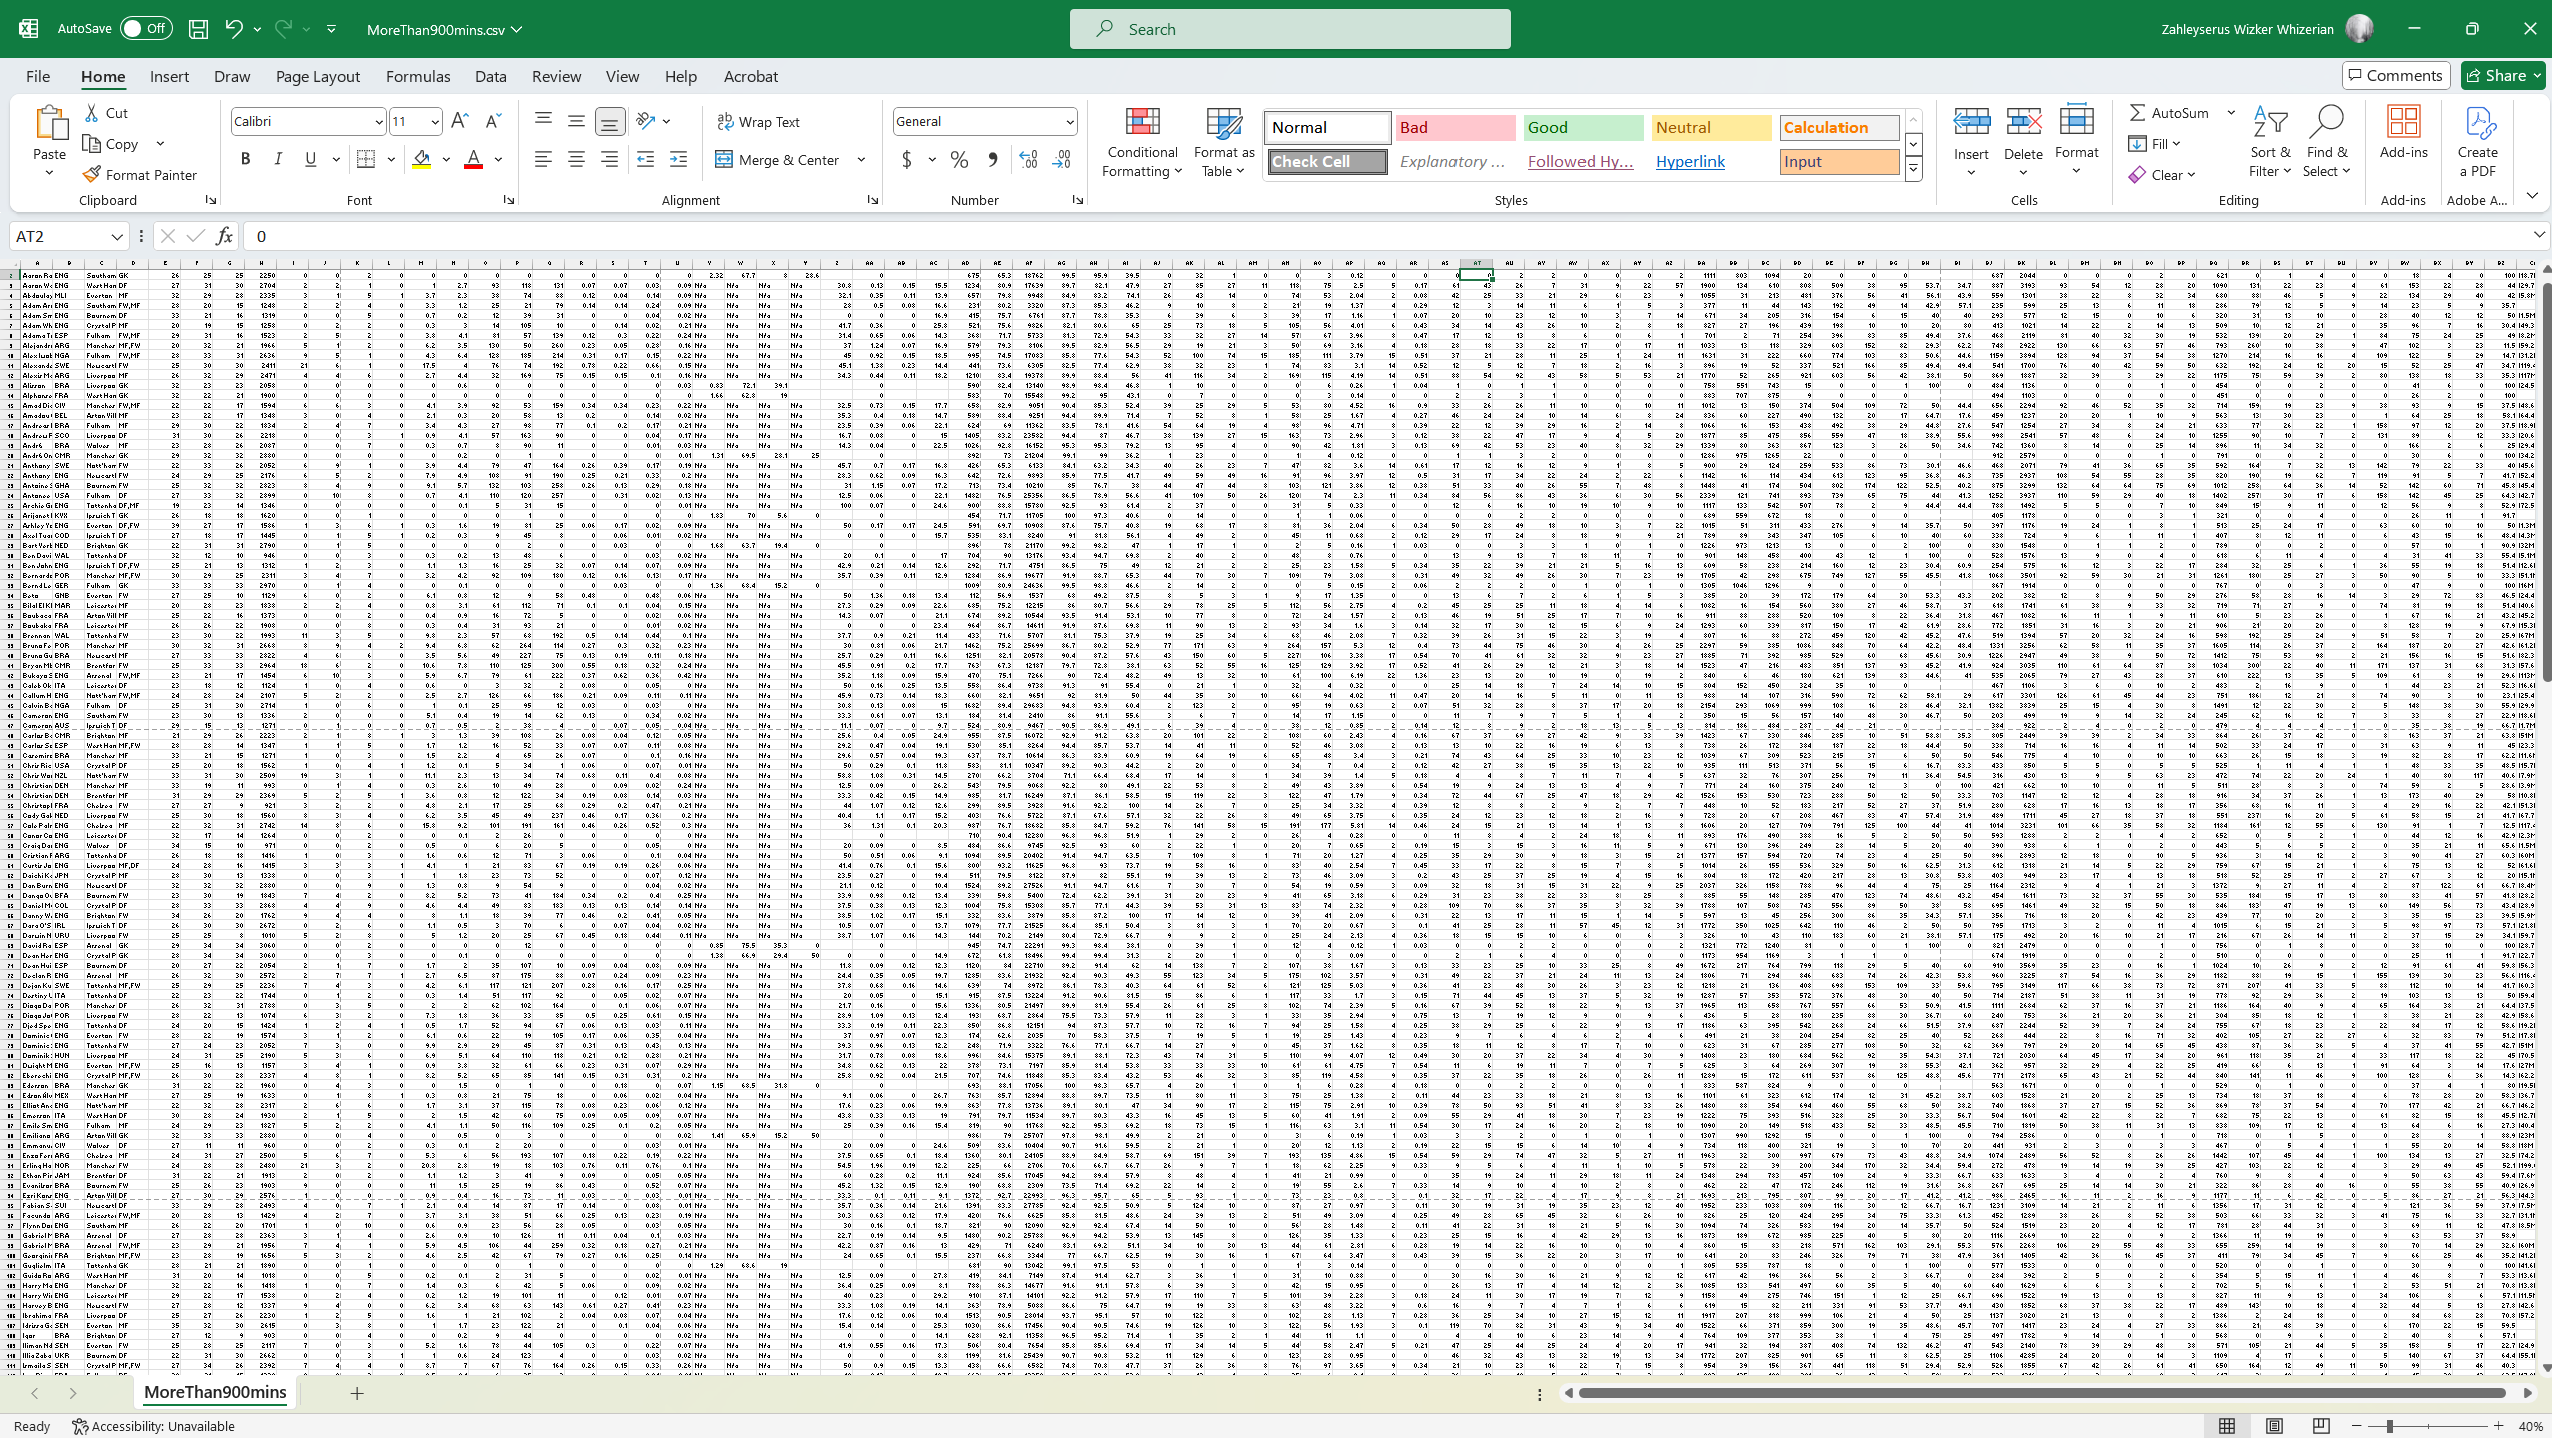
\includegraphics[width=350px]{P4_RES.png}
    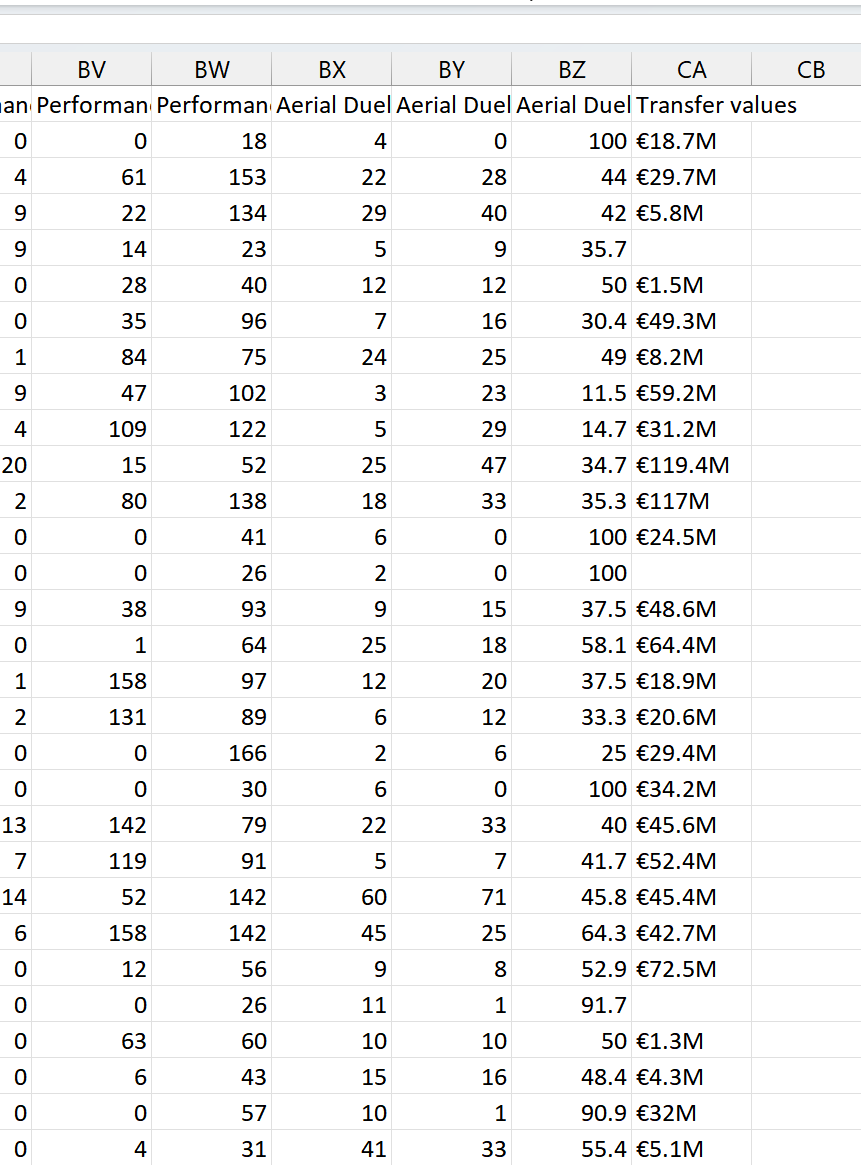
\includegraphics[width=300px]{P41_RES.png}
    \caption{File MoreThan900mins.csv}
    \label{fig:res2}
\end{figure}
The file "MoreThan900mins.csv" is a dataset containing detailed information about football players who have played at least 900 minutes in the season[cite: 459]. The data includes 100 players with 93 different attributes, recording statistics related to performance, individual stats, and general information such as name, nationality, team, position, age, transfer value, along with detailed metrics like playing time, goals scored, assists, yellow/red cards, expected stats (xG, xAG), and many other indicators related to passing ability, defense, attack, and ball control[cite: 460]. \\
The data is organized in CSV format, with each row representing a player and each column a specific attribute[cite: 461]. Attributes include both basic information (e.g., name, team) and in-depth metrics[cite: 462]. This file can be used to analyze player performance, compare across positions, or assess potential in transfer scenarios[cite: 463]. \\
This file has been expanded with a 'Transfer Values' column, with units in millions of euros[cite: 464].
\clearpage
\subsubsection{Evaluation}
The main part affecting execution time and memory usage in the active tasks is the `update\_data` function[cite: 465]. This function performs data crawling from a website using Selenium to control a Chrome browser and BeautifulSoup to parse HTML[cite: 466]. This web scraping process is inherently time-consuming due to factors like network latency, page load times, and browser processing time[cite: 467]. The use of `time.sleep(2)` within the data collection loop also significantly contributes to the total runtime, intended to wait for page content to load completely or to avoid being blocked by the server[cite: 468]. This increases the stability of the crawling process but significantly extends the execution time[cite: 469]. In terms of memory, initializing and maintaining a browser instance (Chrome) via Selenium consumes a considerable amount of memory[cite: 470]. However, the data processing operations using BeautifulSoup and storage in the `player\_dic` dictionary do not seem to put significant pressure on memory for the current data scale, based on the previously reported memory usage results[cite: 471]. The `get\_data` and `save\_result` functions use the pandas library to read, filter, and write data to a CSV file[cite: 472]. Operations with pandas can consume memory, especially with large datasets[cite: 473]. However, in this case, based on the peak memory usage reported from the terminal, it appears the data scale being processed is not excessively large, thus the impact of pandas on memory usage is acceptable[cite: 474]. In summary, for the currently active code section (`Task\_1`), the primary factor governing runtime is the web scraping process within the `update\_data` function due to dependencies on the network, browser, and deliberate pauses (`time.sleep`)[cite: 475]. Memory usage is mainly related to the Selenium browser instance and temporary data structures, but overall appears efficient for the current data scale[cite: 476]. The time and memory usage measurements using `time` and `tracemalloc` at the end of the script provide useful quantitative data for monitoring the overall performance of the program[cite: 477].
\section{Handling Requirement 2}
\subsection{Choosing Model and Features for Processing}
\subsubsection{Model Selection}
Random Forest Regressor is a supervised machine learning algorithm belonging to the class of Ensemble Learning methods, developed by Leo Breiman and Adele Cutler[cite: 478]. It inherits and improves upon the Bootstrap Aggregating (Bagging) technique, primarily aimed at enhancing prediction accuracy and controlling the overfitting phenomenon often encountered in single decision tree models[cite: 479]. This algorithm is particularly effective for regression problems, where the goal is to predict a continuous output value[cite: 480].\\
\textbf{Foundation: Bagging and Decision Trees}
\textbf{Decision Tree}: These are the base estimators in Random Forest[cite: 480]. A regression decision tree works by partitioning the feature space into smaller rectangular regions through a series of split rules based on feature values[cite: 481]. At each leaf node, the predicted value is typically the average of the target values of the training samples belonging to that leaf[cite: 482]. Single decision trees tend to have high variance, are very sensitive to small changes in the training data, and are prone to overfitting[cite: 483].
\textbf*{Bagging (Bootstrap Aggregating)}: This is a general technique in ensemble learning aimed at reducing the variance of an estimator[cite: 484]. It involves two main steps:

\begin{itemize}
    \item \textbf{Bootstrap Sampling}: Generate B new training datasets (bootstrap samples) from the original training dataset by random sampling with replacement[cite: 485]. Each bootstrap sample may contain duplicate data points and omit others[cite: 486]. On average, about 63.2% of the original data points will be present in a specific bootstrap sample[cite: 487].
    \item \textbf{Aggregating}: Train a base estimator (e.g., a decision tree) on each bootstrap sample[cite: 488]. For regression problems, the prediction is averaged from the B base estimators:
    \[
    \hat{f}_{\text{bagging}}(x) = \frac{1}{B} \sum_{b=1}^{B} \hat{f}_b(x)
    \]
    where $\hat{f}_b(x)$ is the prediction from the $b$-th tree trained on the $b$-th bootstrap sample[cite: 489].
\end{itemize}

\textbf*{Core Improvement: Random Subspace Method}
Random Forest enhances Bagging by adding a layer of randomization called the Random Subspace Method (or feature bagging)[cite: 490]. When building each tree on a bootstrap sample $D_b$, at each node needing a split, the algorithm randomly selects only a subset of $m$ features (with $m < p$)[cite: 491]. The search for the best split point is performed only among the $m$ selected features[cite: 492].
\textbf{Parameter $m$}: This is a crucial hyperparameter, typically chosen as $m \approx \frac{p}{3}$ for regression problems[cite: 493]. Choosing a small $m$ helps reduce the correlation between trees in the forest[cite: 494].
\textbf{Reason for Reducing Correlation}: In standard Bagging, if strong features exist, they might be frequently selected in different trees, causing correlation[cite: 495]. Reducing the correlation between trees helps decrease the overall variance of the model without significantly increasing bias[cite: 496].
\textbf*{Random Forest Regressor Algorithm}
Given a training set $D = \{(x_1, y_1), ..., (x_N, y_N)\}$, number of trees $B$, and number of features at each node $m$:

\begin{enumerate}
    \item \textbf{For} $b = 1$ to $B$:
    \begin{enumerate}
        \item Create bootstrap sample $D_b$ by random sampling with replacement from $D$[cite: 497].
        \item Build regression tree $T_b$ on $D_b$:
        \begin{itemize}
            \item At each node: randomly select $m$ features from the $p$ available features[cite: 498].
            \item Find the best split point among the $m$ selected features.
            \item Split the node into two child nodes[cite: 499].
        \end{itemize}
        \item Continue until a stopping criterion is met (e.g., minimum number of samples at a leaf node)[cite: 500].
    \end{enumerate}
    \item \textbf{Output}: The ensemble of trees $\{T_b\}_{b=1}^{B}$[cite: 501].
    \item \textbf{Prediction}: For a new point $x$, the prediction is:
    \[
    \hat{f}_{\text{RF}}(x) = \frac{1}{B} \sum_{b=1}^{B} T_b(x)
    \]
\end{enumerate}

\textbf*{Academic Advantages}
\begin{itemize}
    \item \textbf{High Accuracy}: Performs well on various types of data[cite: 502].
    \item \textbf{Resistant to Overfitting}: Reduces variance thanks to Bagging and random subspace[cite: 503].
    \item \textbf{Handles High-Dimensional Data Well}: Works effectively even when $p > N$[cite: 504].
    \item \textbf{Internal Error Estimation (Out-of-Bag Error)}: Allows error estimation without needing a separate test set[cite: 505].
    \item \textbf{Feature Importance Measurement}: Indicates the importance level of each feature[cite: 506].
\end{itemize}

\textbf*{Academic Disadvantages}
\begin{itemize}
    \item \textbf{Low Interpretability}: Considered a "black box" model[cite: 507].
    \item \textbf{High Computational Cost}: Requires significant resources, especially with large $B$[cite: 508]. However, training can be parallelized[cite: 509].
\end{itemize}

\textbf*{Reason for Model Selection (RandomForestRegressor):}
\begin{itemize}
    \item \textbf{Regression Task}: The goal is to predict a continuous numerical value (e.g., player transfer value), thus requiring a regression model[cite: 510]. Random Forest Regressor is a natural and effective choice in this context[cite: 511].
    \item \textbf{Ability to Handle Non-linearity}: The relationship between features like age, technical stats, and market value is often non-linear[cite: 512]. For instance, a player's value might increase with age when young, peak at a certain age, and then gradually decrease[cite: 513]. Random Forest can effectively model these complex non-linear relationships[cite: 514].
    \item \textbf{Good Predictive Performance}: Random Forest often yields accurate prediction results across various datasets without requiring extensive parameter tuning[cite: 515]. It is a robust and reliable model for many practical problems[cite: 516].
    \item \textbf{Robustness to Outliers and No Need for Scaling}: Random Forest models are less sensitive to outliers and do not require scaling of input features[cite: 517]. This simplifies the data preprocessing workflow[cite: 518].
    \item \textbf{Categorical Feature Handling}: After categorical features are encoded (e.g., using One-Hot Encoding), Random Forest can handle them well and leverage the information they provide[cite: 519].
    \item \textbf{Feature Importance Estimation}: The model can assess the impact of each feature on the prediction outcome, providing deeper insights into the factors determining player value[cite: 520].
    \item \textbf{Alternative Choices}: While other models like Gradient Boosting (XGBoost, LightGBM, CatBoost), Support Vector Regression (SVR), or Neural Networks could also be applied, Random Forest serves as a solid starting point, being easy to implement and commonly used in practice[cite: 521].
\end{itemize}
\subsubsection{Feature Selection}
Beyond analyzing the collected data, selecting the features that most significantly impact player value requires researching various sources[cite: 522], especially scientific papers and research studies, to choose the best features[cite: 523]. Through research, several key features affecting player transfer value have been identified:
\begin{enumerate}
    \item \textbf{Age}: Continuous numerical feature[cite: 524]. Age often non-linearly affects player value, potentially peaking at a certain age and then declining[cite: 525].
    \item \textbf{Position}: Categorical feature describing the player's tactical role on the field (e.g., forward, defender, midfielder)[cite: 526]. Converted to numerical form using One-Hot Encoding (OneHotEncoder) to suit the machine learning model[cite: 527].
    \item \textbf{Playing Time: minutes} (Total minutes played): Continuous numerical feature, reflecting the player's usage level during the season – often positively correlated with market value[cite: 528].
    \item \textbf{Performance: goals} (Number of goals): Numerical feature representing the number of goals scored by the player[cite: 529]. This is a crucial metric, especially for attacking players[cite: 530].
    \item \textbf{Performance: assists} (Number of assists): Numerical feature indicating the ability to assist goals[cite: 531]. Along with goals, this is a key measure of contribution to the attack[cite: 532].
    \item \textbf{GCA: GCA} (Goal-Creating Actions): Continuous numerical feature, representing the number of actions directly leading to a goal (e.g., key passes, dribbles past opponents before a goal)[cite: 533]. It is a composite index for creativity[cite: 534].
    \item \textbf{Progression: PrgR} (Progressive Receptions): Numerical feature measuring the number of times a player receives the ball in progressively valuable (forward-moving) positions[cite: 535]. Reflects tactical movement and receiving ability[cite: 536].
    \item \textbf{Tackles: Tkl} (Number of successful tackles): Numerical feature representing defensive ability, particularly important for defensive players like defenders or defensive midfielders[cite: 537].
\end{enumerate}
This feature set includes both quantitative and qualitative information, selected to cover various aspects of gameplay and performance, from attack and support to defense[cite: 538]. Feature selection is a crucial step in the machine learning model building process, especially for regression problems in the context of sports data[cite: 539]. The features selected in the model are highly relevant based on the following criteria:

\begin{itemize}
    \item \textbf{Relevance}: The selected features are common statistical indicators with clear domain expertise backing in football[cite: 540]. Specifically, age, position, playing time, goal-scoring and assisting ability, attacking support metrics (GCA, PrgR), as well as defensive metrics (Tkl) directly reflect performance and thus influence the player's market value[cite: 541].
    \item \textbf{Availability}: These features represent commonly collected and easily accessible data, often found in major football databases like FBref, Opta, or StatsBomb[cite: 542]. This ensures feasibility when deploying the model in practice[cite: 543].
    \item \textbf{Diversity}: The feature set covers multiple dimensions: personal information (age, position), playing time (minutes), attacking ability (goals, assists, GCA, PrgR), and defensive ability (Tkl)[cite: 544]. This provides a comprehensive view of a player's capabilities from both tactical and statistical perspectives[cite: 545].
    \item \textbf{Practical Note}: Feature selection is not entirely fixed but often involves experimentation and adjustment[cite: 546]. It might initially rely on domain knowledge, exploratory data analysis, or automated techniques like Recursive Feature Elimination or feature importance derived from tree-based models[cite: 547]. The effectiveness of the feature set is evaluated using model evaluation metrics such as MAE, RMSE, or R-squared[cite: 548].
\end{itemize}
\subsection{Actual Code and Description}
\begin{lstlisting}
def estimate_player_value(file_path):
    # Load data
    df = pd.read_csv(file_path)

    # Clean minutes column if necessary
    if df['Playing Time: minutes'].dtype == object:
        df['Playing Time: minutes'] = df['Playing Time: minutes'].str.replace(',', '').astype(int)

    # Fix Transfer values format to int
    df = df.dropna(subset=['Transfer values'])
    df['Transfer values'] = df['Transfer values'].str.replace('€', '', regex=False).str.replace('M', '', regex=False).astype(float) * 1_000_000
    df['Transfer values'] = df['Transfer values'].astype(int)

    # Select features
    features = [
        'Age',
        'Position',
        'Playing Time: minutes',
        'Performance: goals',
        'Performance: assists',
        'GCA: GCA',
        'Progression: PrgR',
        'Tackles: Tkl'
    ]

    X = df[features]
    y = df['Transfer values']

    # Split data
    X_train, X_test, y_train, y_test = train_test_split(X, y, test_size=0.2, random_state=42)

    # Preprocessing: OneHot for categorical 'Position'
    categorical_features = ['Position']
    numeric_features = [col for col in features if col not in categorical_features]

    preprocessor = ColumnTransformer(
        transformers=[
            ('cat', OneHotEncoder(handle_unknown='ignore'), categorical_features)
        ],
        remainder='passthrough' # Numeric features stay unchanged
    )

    # Model
    model = RandomForestRegressor(n_estimators=100, random_state=42)

    # Pipeline
    pipeline = Pipeline(steps=[
        ('preprocessor', preprocessor),
        ('model', model)
    ])

    # Train
    pipeline.fit(X_train, y_train)

    # Predict and evaluate
    y_pred = pipeline.predict(X_test)
    mae = mean_absolute_error(y_test, y_pred)
    print(f"Mean Absolute Error: {mae:,.0f} €")

    return pipeline
\end{lstlisting}
This function implements a workflow to build and evaluate a Machine Learning model for estimating the transfer value of football players based on their statistics[cite: 553].
\textbf{Workflow}

\textbf{1. Load Data}:
\begin{verbatim}
df = pd.read_csv(file_path)
\end{verbatim}
The function reads data from a CSV file (specified by `file_path`) into a pandas DataFrame named `df`[cite: 554].

\textbf{2. Clean Data}:
\textbf{Process 'Playing Time: minutes' column}:
Checks the data type of the 'Playing Time: minutes' column. If it's 'object' (string), removes commas and converts the data type to integer:
\begin{verbatim}
df['Playing Time: minutes'] = df['Playing Time: minutes'].str.replace(',', '').astype(int)
\end{verbatim}

\textbf{Process 'Transfer values' column}:
Removes missing values (NaN) and converts transfer values from string (e.g., "€50.5M") to float, then integer:
\begin{verbatim}
df = df.dropna(subset=['Transfer values'])
df['Transfer values'] = df['Transfer values'].str.replace('€', '', regex=False).str.replace('M', '', regex=False).astype(float) * 1_000_000
df['Transfer values'] = df['Transfer values'].astype(int)
\end{verbatim} [cite: 549]

\textbf{3. Select Features (Input Variables)}:
Selects features that influence player transfer value:
\begin{verbatim}
features = ['Age', 'Position', 'Playing Time: minutes', 'Performance: goals', 'Performance: assists', 'GCA: GCA', 'Progression: PrgR', 'Tackles: Tkl']
X = df[features]
y = df['Transfer values']
\end{verbatim} [cite: 555]

\textbf{4. Split Data}:
Splits the data into training and testing sets with an 80/20 ratio:
\begin{verbatim}
from sklearn.model_selection import train_test_split
X_train, X_test, y_train, y_test = train_test_split(X, y, test_size=0.2, random_state=42)
\end{verbatim} [cite: 556]

\textbf{5. Preprocessing}:
Handles categorical and numerical features:
\begin{verbatim}
from sklearn.compose import ColumnTransformer
from sklearn.preprocessing import OneHotEncoder

categorical_features = ['Position']
numeric_features = ['Age', 'Playing Time: minutes', 'Performance: goals', 'Performance: assists', 'GCA: GCA', 'Progression: PrgR', 'Tackles: Tkl']

preprocessor = ColumnTransformer(
    transformers=[
        ('cat', OneHotEncoder(handle_unknown='ignore'), categorical_features),
        ('num', 'passthrough', numeric_features)
    ])
\end{verbatim} [cite: 557]

\textbf{6. Select and Initialize Model}:
Uses the RandomForestRegressor model with 100 decision trees:
\begin{verbatim}
from sklearn.ensemble import RandomForestRegressor
model = RandomForestRegressor(n_estimators=100, random_state=42)
\end{verbatim} [cite: 558]

\textbf{7. Create Pipeline}:
Combines preprocessing steps and the model into a Pipeline:
\begin{verbatim}
from sklearn.pipeline import Pipeline
pipeline = Pipeline(steps=[
    ('preprocessor', preprocessor),
    ('model', model)
])
\end{verbatim} [cite: 559]

\textbf{8. Train Model}:
Trains the model using the training data:
\begin{verbatim}
pipeline.fit(X_train, y_train)
\end{verbatim} [cite: 560]

\textbf{9. Predict and Evaluate}:
Predicts transfer values and evaluates the model using Mean Absolute Error (MAE):
\begin{verbatim}
from sklearn.metrics import mean_absolute_error
y_pred = pipeline.predict(X_test)
mae = mean_absolute_error(y_test, y_pred)
print(f"Mean Absolute Error: {mae:,.0f} €")
\end{verbatim} [cite: 561, 552]

\textbf{10. Return Result}:
Returns the trained model:
\begin{verbatim}
return pipeline
\end{verbatim} [cite: 562]

\subsection{Testing and Evaluation}
\textbf{Testing}\\
\begin{lstlisting}
def Task_2():
    # Example usage
    model = estimate_player_value('MoreThan900mins.csv')

    new_player = pd.DataFrame({
        'Age': [26],
        'Position': ['GK'],
        'Playing Time: minutes': [2250],
        'Performance: goals': [0],
        'Performance: assists': [0],
        'GCA: GCA': [0],
        'Progression: PrgR': [0],
        'Tackles: Tkl': [0]
    })

    # Predict the value of the new player
    predicted_value = model.predict(new_player)
    print(f"Estimated player value: {predicted_value[0]:,.0f} €")
\end{lstlisting} [cite: 563]
\begin{figure}[h]
    \centering
    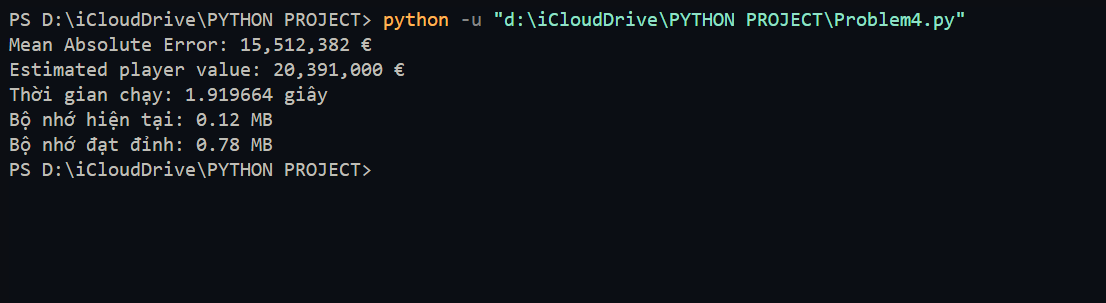
\includegraphics[width=300px]{Terminal_41.png}
    \caption{Terminal after executing function Task\_2}
    \label{fig:res4}
\end{figure}
The results show a completion time of approximately 1.92 seconds and peak memory consumption of 0.78 MB, along with specific calculation results like Mean Absolute Error and Estimated player value[cite: 565]. From an academic perspective, the execution environment is presented through a standard command-line interface with a dark theme[cite: 566]. Analysis of the results indicates the Python script achieved a runtime performance of approximately 1.92 seconds and notable memory efficiency, requiring a maximum of only 0.78 MB, providing important empirical data for evaluating and optimizing the program's resource performance[cite: 567].
\textbf{Evaluation}\\
Analysis of the `Problem4.py` source code and execution results reveals that the program focuses on building a machine learning model to predict player values based on statistical features[cite: 568]. Stable and efficient components include the initial data processing workflow (loading, basic cleaning of numerical columns), feature selection, dataset splitting, and particularly the implementation of a machine learning pipeline using scikit-learn[cite: 569]. This pipeline combines preprocessing of categorical data using One-Hot Encoding via `ColumnTransformer` and the `Random Forest` regression model[cite: 570]. Execution results from the terminal confirm the dynamic functionality of this pipeline, displaying a Mean Absolute Error (MAE) of **€15,512,382**, a quantitative measure of the model's accuracy on the test dataset[cite: 571]. The estimated player value for a specific case is **€20,391,000**[cite: 572]. The program also integrates performance measurement functionality, recording a runtime of approximately **1.92 seconds** and peak memory usage of **0.78 MB**, indicating relative resource efficiency for the data scale processed in this run[cite: 573].
\textbf{Advantages of the source code:}
\begin{itemize}
    \item \textbf{Modularity}: The code is organized into separate functions for distinct tasks (get data, update data, save results, build model, specific tasks), enhancing readability and maintainability[cite: 574].
    \item \textbf{Use of Strong Standard Libraries}: Effectively leverages popular and highly optimized libraries like `pandas` for data handling, `scikit-learn` for machine learning (including `Pipeline`, `ColumnTransformer`, `RandomForestRegressor`), and `time`/`tracemalloc` for performance analysis[cite: 575].
    \item \textbf{ML Pipeline Implementation}: Using Pipeline and ColumnTransformer is a good practice for systematically handling preprocessing steps and modeling, helping to prevent data leakage between steps, which is particularly important during model evaluation[cite: 576].
    \item \textbf{Integrated Performance Measurement}: Adding code snippets to measure runtime and memory usage is a major plus, providing necessary information to evaluate and optimize the program's resource efficiency[cite: 577].
\end{itemize}

\textbf{Disadvantages of the source code:}
\begin{itemize}
    \item \textbf{Accuracy}: The MAE of **€15,512,382** is a specific number, but assessing whether this accuracy is "high" or low depends on the problem context (range of transfer values, data variability, comparison with other models or baselines)[cite: 578]. Without further comparison information, it's difficult to conclude the model's true effectiveness[cite: 579].
    \item \textbf{Dependency on External Data Source}: The `update_data` function heavily relies on the HTML structure of the `footballtransfers.com` website[cite: 580]. Any changes to the website could break the data crawling functionality, making this part less robust[cite: 581].
    \item \textbf{Lack of Robust Error Handling}: Although basic `try...except` handling exists in the crawling part, the code lacks more comprehensive error handling mechanisms for cases like non-existent input files, incorrect data formats, or connection errors during crawling[cite: 582].
    \item \textbf{Lack of Deeper Model Tuning and Evaluation}: The code uses only one model type (`RandomForestRegressor`) with default parameters (`n_estimators=100`) and evaluates on a single data split (`test_size=0.2`)[cite: 583]. Exploring other models, hyperparameter tuning, and using Cross-validation would provide a more reliable evaluation and potentially improve model performance[cite: 584].
    \item \textbf{Fixed File Paths}: Input and output file paths are hardcoded, reducing the code's flexibility and reusability on different systems or directory structures[cite: 585].
\end{itemize}

\textbf{In summary}, the source code demonstrates an understanding of the data processing and machine learning model building workflow using standard libraries[cite: 586]. The core parts related to the ML pipeline and performance measurement function well[cite: 587]. However, the dependency on an unstable external data source, lack of comprehensive error handling, and insufficient model evaluation are areas for improvement[cite: 588].

\chapter*{Conclusion}
{
\noindent
This report has presented the process of performing a series of football data analysis tasks using the Python programming language, focusing on collecting, processing, analyzing, and modeling player statistical data from the 2004--2005 English Premier League season and recent transfer data[cite: 589].
\vspace{1em}
\noindent
\textbf{Summary of Key Results:}

\vspace{0.5em}
\noindent
\textit{Data Collection and Preprocessing (Problem I):} Successfully collected detailed statistical data for 491 players playing over 90 minutes from \texttt{fbref.com} using web scraping techniques with Selenium and BeautifulSoup[cite: 590]. Data was cleaned, standardized (unavailable values marked as "N/a"), and stored structurally in the \texttt{results.csv} file[cite: 591]. This process ensured data accuracy and completeness but showed suboptimal time performance (~186 seconds) due to multiple browser initializations[cite: 592]. However, memory usage was quite efficient (~32.74 MB)[cite: 593].
\vspace{0.5em}
\noindent
\textit{Descriptive Statistical Analysis (Problem II):} Conducted further analysis on the \texttt{results.csv} file[cite: 594]. Identified the top 3 players with the highest and lowest stats for each metric (saved in \texttt{top\_3.txt})[cite: 595]. Calculated important descriptive statistics (median, mean, standard deviation) for the entire league and each team (saved in \texttt{results2.csv})[cite: 596]. Visualized the distribution of key metrics through histograms (saved as PNG files)[cite: 597]. Based on the number of leading metrics, Liverpool was identified as the team with the best overall performance (leading in 28 metrics, results saved in \texttt{best\_team\_summary.txt})[cite: 598]. This analysis provided a multi-dimensional view of player and team performance, although the method for identifying the best team was relatively simple[cite: 599].
\vspace{0.5em}
\noindent
\textit{Player Clustering (Problem III):} Applied the K-means algorithm to group players based on statistical data[cite: 600]. The optimal number of clusters was determined to be $K=6$ using the Elbow method and Silhouette Score, consistent with actual football position groups[cite: 601]. PCA technique was used to reduce data dimensionality to 2 dimensions, allowing for effective visualization of player clusters[cite: 602]. Analysis of the characteristics of each cluster revealed similarities in roles or playing styles among players within the same group (analysis results and plots saved in the \texttt{P3\_RES} directory)[cite: 603]. Although K-means and PCA have certain limitations (assumptions about cluster shape, information loss), this method provided useful initial insights into the underlying structure of player data[cite: 604].
\vspace{0.5em}
\noindent
\textit{Player Value Estimation (Problem IV):} Collected transfer value data from \texttt{footballtransfers.com} for players playing over 900 minutes (saved in \texttt{MoreThan900mins.csv})[cite: 605]. Successfully proposed and implemented a \texttt{RandomForestRegressor} model to estimate player value[cite: 606]. Important input features such as Age, Position, Playing Time, Goals, Assists, GCA, PrgR, Tkl were selected based on domain knowledge and research[cite: 607]. The model achieved a Mean Absolute Error (MAE) of approximately €15.5 million on the test set[cite: 608]. Using \texttt{Pipeline} in Scikit-learn helped systematize the preprocessing and training workflow[cite: 609]. However, the model still depends on external data sources and needs improvement in accuracy and deeper evaluation (e.g., hyperparameter tuning, using cross-validation)[cite: 610].
\vspace{1em}
\noindent
\textbf{Overall Assessment:}

\vspace{0.5em}
\noindent
Overall, the project successfully met the stated objectives, demonstrating the ability to apply data science techniques from collection, processing, analysis to modeling in the sports domain[cite: 611]. The effective use of Python libraries such as \texttt{Pandas}, \texttt{Scikit-learn}, \texttt{Selenium}, \texttt{BeautifulSoup} is a notable strength[cite: 612]. The analysis and modeling results provide valuable information about player performance, team characteristics, and factors influencing transfer values[cite: 613].
\vspace{0.5em}
\noindent
However, there are still areas for improvement, such as optimizing web scraping speed, developing more complex composite evaluation metrics, and performing more comprehensive model evaluation[cite: 614]. The dependency on the structure of external websites is also a weakness to note regarding the sustainability of the data collection solution[cite: 615].
\vspace{0.5em}
\noindent
In conclusion, this report serves as a testament to the powerful application of Python and machine learning techniques in exploring and extracting knowledge from complex football data[cite: 616].
}

\chapter*{References}
{
\begin{enumerate}
    \item Scikit-learn Developers. (n.d.). RandomForestRegressor. Scikit-learn documentation.
    \item GeeksforGeeks. (n.d.). Random Forest Regression in Python[cite: 617].
    \item Université du Luxembourg. (2020). Random Forest Regression [Project Report].
    \item StatQuest with Josh Starmer. (n.d.). Random Forests Part 1: Regression [Video]. YouTube[cite: 618].
    \item Metelski, Adam. (2021). Factors affecting the value of football players in the transfer market. Journal of Physical Education and Sport. 21. 1150-1155. 10.7752/jpes.2021.s2145[cite: 619].
    \item Rong, Zhangyi, Wang, Lujie, \& Xie, Shengting. (2024). \textit{Factors that Influence Player Market Value in Different Position: Evidence from European Leagues}. Advances in Economics, Management and Political Sciences, 82, 50--63[cite: 620, 621].
    \item Football Benchmark. (n.d.). Game changers: A snapshot of the top 100 most valuable players. Football Benchmark[cite: 622].
    \item Zhang, Y., \& Zhang, W. (2019). \textit{Research on player value evaluation model based on multiple linear regression analysis}[cite: 623].
    \item Krabbenborg, L. (2020). The relationship between player market value and performance in professional European football: A statistical analysis (Bachelor's thesis, Tilburg University)[cite: 624].

\end{enumerate}
}
\end{document}